\chapter{Identyfikacja cech dynamicznych konstrukcji}

\textit{Streszczenie: W niniejszym rozdziale przytoczono klasyfikację metod analizy modalnej. W dalszej części skupiono uwagę na Operacyjnej Analizie Modalnej. Przedstawiono generalne założenia OMA oraz zastosowania udokumentowane w literaturze. Następnie opisano wybrany do wykorzystania w pracy algorytm NExT-ERA. Przedstawiono jego syntetyczną formę wraz z zaleceniami dotyczącymi użycia. W dalszej części rozdziału opisano stworzoną do identyfikacji modalnej aplikację komputerową korzystającą z algorytmu NExT-ERA. Na końcu przedstawiono testy numeryczne oraz eksperymentalne metody i aplikacji komputerowej.}

\textbf{Przerzucić tutaj wstępu z dynamiki.}

\section{Operacyjna analiza modalna (OMA)}
\subsection{Koncepcja OMA}
W ogólności doświadczalna analiza modalna to proces korelacji charakterystyk dynamicznych modelu matematycznego, z fizycznymi właściwościami systemu opisanego rezultatami pomiarów. Przypomnijmy, że w OMA do procesu estymacji parametrów modalnych używane są tylko pomiary odpowiedzi konstrukcji. Różni ją to od EMA, w której mierzone są zarówno wymuszenia jak i odpowiedź. 
Fundamentem wszystkich metod OMA jest założenie, że badana struktura obciążona jest wymuszeniem o widmie zbliżonym do białego szumu. Oznacza to, żę energia konstrukcji jest rozłożona w szerokim paśmie częstotliwości, które zawiera wszystkie interesuje badacza mody do identyfikacji. Z oczywistych względów idealne wymuszenie o charakterystyce białego szumu nie jest możliwe. Większość metod radzi sobie z tym brakiem, jednak najważniejsze jest, żeby wszystkie interesujące mody były odpowiednio wzbudzone, tak aby ich wkład był wychwycony przez przyrządy pomiarowe. \cite{Brincker2015} tłumaczą tę koncepcję za pomocą fikcyjnego, kolorowego filtru obciążenia. Zaproponowano, że kolorowe obciążenie może być traktowanego jako wynik obciążenia kolorowego filtru (zgodnego z obciążeniem) przez idealnie biały szum. Udowodniono, że takie podejście nie zmienia fizycznych modów systemu. Należy jednak pamiętać, że metody OMA w tym przypadku dokonają identyfikacji modalnej zarówno struktury fizycznej, jak i filtra obciążenia. Koncepcję zaprezentowano na rysunku \ref{fig: color_filter_oma}. Najważniejszą konsekwencją jest możliwość występowania wśród wyników identyfikacji nie tylko modów związanych z konstrukcją, ale też wynikających z warunków obciążenia. Należy pamiętać również, że pomierzone wartości obarczone są szumem pomiarowym. Nie niesie on żadnej istotnej, fizycznej informacji, ale jest nieunikniony w trakcie rzeczywistych pomiarów. Tak więc wynik identyfikacji zawiera w sobie trzy składowe:
\begin{itemize}[noitemsep]
	\item parametry modalne związane z drganiami własnymi konstrukcji,
	\item myślowy filtr obciążenia, kolorujący biały szum do rzeczywistego, nieznanego obciążenia,
	\item szum pomiarowy.
\end{itemize} 
W idealnych warunkach, kiedy filtr obciążenia ma biały kolor, a szum pomiarowy byłby zerowy, OMA zidentyfikuje wyłącznie mody konstrukcji.
\begin{figure}[h] 
	\centering
	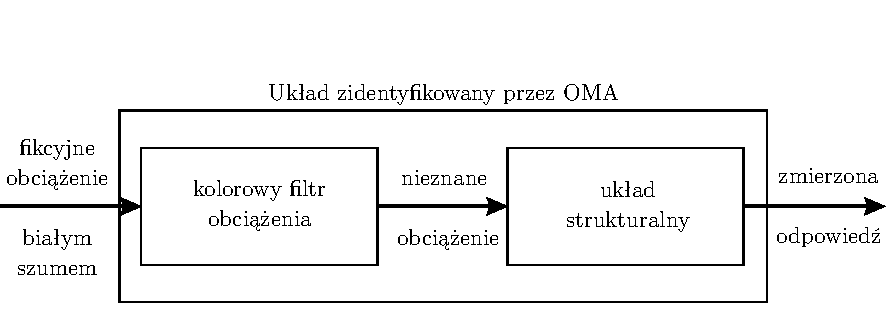
\includegraphics[]{/modal_analysis/filter_coloring.pdf}
	\captionsetup{justification=centering}
	\caption{Schemat układu identyfikowanego przez OMA przy koncepcji kolorowego filtru obciążenia}
	\label{fig: color_filter_oma}
\end{figure}

Operacyjna Analiza Modalna jest obwarowana pewnymi założeniami. Są one rozwinięciem założeń podanych w punkcie \ref{section: modalAnalysisIntro}. Układ poddany analizie OMA musi spełniać następujące warunki:
\begin{itemize}
	\item liniowość - odpowiedź układ na zadaną kombinację obciążeń, jest sumą odpowiedzi odpowiadających każdemu obciążeniu traktowanemu osobno - zasada superpozycji,
	\item stacjonarność - charakterystyki dynamiczne konstrukcji nie zmieniają się w czasie. Innymi słowy, współczynniki równań różniczkowych opisujących odpowiedź struktury są niezależne od czasu.
	\item obserwowalność - dobór lokalizacji punktów pomiarowych musi być tak zaprojektowany, żeby był w stanie dostrzec interesujące obserwatora mody. Niezależnie od tego w trakcie analizy spełnione muszą być również kryteria obserwowalności sterowalności opisane w punkcie \ref{section: hankelMatrix}.
\end{itemize}


\subsection{Metody operacyjnej analizy modalnej}

Metody identyfikacji modalnej dzielą się na dwa główne rodzaje związane z dziedziną w której działa algorytm:
\begin{itemize}[noitemsep]
	\item metody w dziedzinie czasu \teng{time-domain methods (TDM)},
	\item metody w dziedzinie częstotliwości \teng{frequency-domain methods (FDM)}.
\end{itemize}
Metody EMA w dziedzinie czasu wykorzystują do estymacji parametrów modalnych funkcje odpowiedzi impulsowej \teng{inpulse response function (IRF)}. W OMA, nośnikiem informacji o odpowiedzi swobodnej układu \teng{free decays} są funkcje korelacji \teng{correlation functions}. Identyfikacja parametrów polega w tym przypadku na dopasowaniu parametrów modalnych do informacji zawartej w funkcjach korelacji. Stosowane są do tego modele parametryczne wykorzystujące techniki regresji. Główną różnicą pomiędzy dostępnymi algorytmami TD jest właśnie zastosowana metoda regresji. Zasadniczo wszystkie metody TD stosowane w EMA mogą być użyte w OMA właśnie z zastosowaniem funkcji korelacji. 


Podobną analogię jak w metodach TD można zauważyć dla metod w dziedzinie częstotliwości. W algorytmach EMA w dziedzinie częstotliwości bazą do identyfikacji są funkcje odpowiedzi częstotliwościowej \teng{frequency-response function (FRF)}. W OMA rolę tę pełnią funkcje gęstości widmowej \teng{spectral density functions}.

Przed wyborem dziedziny w której badacz chce się poruszać, warto poznać elementy charakterystyczne dla grupy algorytmów TD i FD. Podstawową wadą metod TD jest to, że wszystkie mody, które występują w sygnale są ujęte w funkcjach korelacji. W konsekwencji wszystkie mody zawsze są rozważane w trakcie rozwiązania problemu. Z kolei ich zaletą, w porównaniu do metod FD, jest większa odporność na wystąpienie błędów systematycznych w estymowanych parametrach modalnych. Niejako w kontrze do metod TD, zaletą metod FD jest to, że każdy z modów występuje w wąskim przedziale częstotliwości. Dzięki temu możliwe jest rozważanie tylko przedziałów częstotliwości, w których występują interesujące badacza mody. Z drugiej strony wadą metod FD jest wykorzystywanie do identyfikacji funkcje gęstości widmowej, które są wyznaczane za pomocą różnych metod (CYTOWANIE) obciążonych błędami systematycznymi. Błędy te nieuchronnie przenoszą się na wynikowe parametry modalne, a określenie ich wpływu jest problematyczne. \cite{Maia1997} sugerują, że metody w dziedzinie czasu są z reguły lepszym wyborem w przypadku dużego przedziału interesujących badacza częstotliwości, albo dużej liczby modów w tym zakresie. Natomiast metody w dziedzinie częstotliwości dostarczają lepszych wyników kiedy zakres częstotliwości jest niewielki, a liczba modów relatywnie mała. 

Drugie kryterium podziału algorytmów dotyczy liczby modów, które mogą być jednocześnie analizowane za pomocą danej metody. Podział jest zbliżony do tego dotyczącego teoretycznej analizy modalnej. Metoda może identyfikować albo jeden stopień swobody \teng{single degree-of-freedom} albo wiele stopni swobody \teng{multiple degree-of-freedom}.

Metody TDM i FDM możemy podzielić również na bezpośrednie \teng{direct} i pośrednie \teng{indirect}. Różnica polega na sposobie wyznaczania FRF. Metody bezpośrednie pozwalają wyznaczyć ją bezpośrednio z równania ruchu. Natomiast metody pośrednie estymują FRF na podstawie wcześniej zidentyfikowanego modelu modalnego.

Ostatnim ogólnie przyjętym kryterium podziału jest liczba punktów poddanych wymuszeniu i mierzonych w trakcie serii pomiarowej. Koresponduje to z liczbą analizowanych jednocześnie przez metodę identyfikacji funkcji FRF. Kiedy mówimy o jednoczesnej analizie tylko jednej funkcji FRF mamy do czynienia z metodą jedno-wejście-jedno-wyjście (SISO) \teng{single-input-single-output}. Kiedy mierzymy wymuszenie w jednym punkcie, a odpowiedź badamy w kilku różnych punktach na konstrukcji, otrzymując kilka funkcji FRF, metodę klasyfikuje się jako jedno-wejście-wiele-wyjść (SIMO) \teng{single-input-multi-output}. W powyższej technice obowiązuje założenie, że parametry modalne uzyskane z każdej funkcji FRF będą takie same. Innymi słowy są to parametry globalne dla całej konstrukcji. Naturalnym rozwinięciem są metody które mogą analizować wszystkie dostępne funkcje FRF jednocześnie, uzyskane w skutek wymuszenia i pomiaru wielu różnych punktów. Metody te określane są jako wiele-wejść-wiele-wyjść (MIMO) \teng{multi-input-multi-output}.

\cite{Maia1997} opisali szczegółowo wiele z metod zarówno eksperymentalnej jaki i doświadczalnej analizy modalnej. Z kolei \cite{Brincker2015} sklasyfikowali najpopularniejsze, używane współcześnie metody identyfikacji OMA. Spośród algorytmów działających w dziedzinie czasu należy wymienić:
\begin{itemize}[noitemsep]
	\item Poly Reference (PR) \parencite{Norton2009,Vold1982},
	\item Autoregressive Moving Average (ARMA) \parencite{Shi1987,Huang2000,Giorcelli1994},
	\item Ibrahim Time Domain (ITD) \parencite{Ibrahim1983,Pappa1985a},
	\item Eigensystem Realization Algorithm (ERA) \parencite{Juang1985,Pappa1985,Juang1988},
	\item Stochastic Subspace Identification (SSI). \parencite{VanOverschee1996,Peeters1999a,Peeters2000}. 
\end{itemize}

Warto zaznaczyć, żę metoda ERA przy zastosowaniu postulatów NExT stanowi jeden z pośrednich wariantów metody SSI, używający funkcji korelacji jako źródła informacji przy identyfikacji.

Z kolei najpopularniejsze algorytmy w dziedzinie częstotliwości to:
\begin{itemize}[noitemsep]
	\item Basic Frequency Domain (Peak-Picking) \parencite{Felber1994},
	\item Frequency-Domain-Decomposition (FDD) \parencite{Brincker2000,Brincker2001a,Brincker2001b},
	\item The Least Squares Complex Frequency Method (LSCF) \parencite{Verboven2005},
	\item The Poly-Reference Least Squares Complex Frequency Method (p-LSCF) \parencite{Peeters2005}.
\end{itemize}



Wszystkie z powyższych algorytmów są bardzo dobrze opisane i udokumentowane w literaturze. Trudno orzec, który z nich jest obiektywnie najlepszy. Wiele zależy od doświadczenia i wiedzy autora oraz specyfiki zadania. Jak powiedział Sam Ibrahim: "Jeśli nie występują blisko położone mody i szumy - wszystko zadziała" \teng{"If there are no closely spaced modes and no noise - everything works"}. Wybór metody może więc zależeć od preferencji, umiejętności programowania czy dostępnych narzędzi. W literaturze można napotkać wiele indywidualnych aplikacji algorytów (CYTOWANIE). Istnieją również komercyjne programy, które pozwala na identyfikację modalną. Do najpopularniejszych należą ARTeMIS - SVS \parencite{Extractor1999} i MACEC - dodatek do programu MATLAB \parencite{Reynders2014}.

Do identyfikacji parametrów modalnych konstrukcji, które są częścią tej pracy autor zdecydował o zastosowaniu algorytmu NExT-ERA. Wynika to z doświadczenia zespołu mostów Politechniki Gdańskiej przy stosowaniu tej metody oraz z dostępnej szerokiej literatury pokazującej skuteczne zastosowanie tej metody w przypadku badania mostów. W kolejnym rozdziale omówiono szczegóły metody oraz implementację jej algorytmu w autorskiej aplikacji napisanej w języku Python.

\section{Przykłady zastosowań Operacyjnej Analizy Modalnej}
Operacyjna analiza modalna została zastosowana w wielu przykładach testowych i przy rozwiązaniu rzeczywistych problemów inżynierskich. Identyfikacja OMA najczęściej służy jako element detekcji zmian i uszkodzeń konstrukcji lub jako punkt odniesienia przy kalibracji modeli numerycznych. Ze względu na swoje właściwości używana jest przy badaniu dużych budowli i konstrukcji, których sztuczne wymuszenie byłoby problematyczne. W literaturze można znaleźć wiele przykładów identyfikacji modalnej rzeczywistych mostów \parencite{L.Hermans1999,Siringoringo2008,Degrauwe2008,Liu2009,Bayraktar2009,Brownjohn2010,Dohler2011,Magalhaes2012,Benedettini2015,Brownjohn2017,Brownjohn2018,Poprawa2018,Barbieri2019,Qin2019,Favarelli2021}, turbin wiatrowych \parencite{Carne2010,Sarrafi2018}, budynków \parencite{Zhu2018,Xie2021}, statków powietrznych \parencite{SHEN2003,Moncayo2010} czy budowli wieżowych \parencite{Cabboi2017,Szafranski2020}. 

\section{Metoda NExT-ERA}
Metoda NExT-ERA jest jedną z metod operacyjnej analizy modalnej. Składnik NExT pochodzi od słów \textbf{N}atural \textbf{Ex}citation \textbf{T}echnique. NExT jest właściwie klasą metodą OMA. Zawiera w sobie algorytmy początkowo stworzone do eksperymentalnej analizy modalnej wejście-wyjście \teng{input-output} (np. ERA, LSCE, ITD), a które następnie rozszerzone zostały do analizy problemu jedynie na podstawie sygnałów odpowiedzi konstrukcji \teng{output-only}. Taką możliwość ujawniło odkrycie faktu, że funkcje korelacji odpowiedzi konstrukcji, wywołanej losowymi wymuszeniami mogą być wyrażone jako suma zanikających sinusoid. Potwierdzono również, że funkcje korelacji zawierają informację na temat parametrów modalnych struktury. Zauważono więc, że można zastąpić tradycyjnie używane funkcje odpowiedzi impulsowej (IRF), funkcjami korelacji losowych drgań konstrukcji pod wymuszeniem środowiskowym. W ten sposób tradycyjne metody EMA zostały skutecznie zaadaptowane do OMA \parencite{Rainieri2014}. W dalszej części rozdziału zostaną przedstawione najważniejsze zagadniania dotyczące identyfikacje metodą NExT-ERA. 

\subsection{Funkcje korelacji, a odpowiedź swobodna układu} \label{sect: correlationFunction}
Przyjmijmy, że $X$ oznacza zmienną losową, a $x(t)$ realizację tej zmiennej losowej w czasie. $x(t)$ w tej pracy może być utożsamiany z zaobserwowanym sygnałem. Wprowadźmy prostą definicję kowariancji. Jest to funkcja, która dostarcza informacji o zależności pomiędzy dwoma zmiennymi i dana jest wzorem:
\begin{equation}
	\mathrm{cov}[X,Y] = \mathrm{E}[XY]=\int_{-\infty}^{\infty}\int_{-\infty}^{\infty}xyp_{xy}(x,y)\,dxdy
\end{equation}
gdzie: $\mathrm{E}[\,]$ - wartość oczekiwana, $p_{xy}(x,y)$ - wspólna funkcja gęstości prawdopodobieństwa \teng{joint probability density function}. Używając metody uśredniania w czasie $[0,T]$ możemy zapisać kowariancję jako:
\begin{equation}
	\mathrm{cov}[x(t),y(t)] = \mathrm{E}[x(t)y(t)]=\frac{1}{T}\int_{0}^{T}x(t)y(t) \,dt
\end{equation}
Korelacją możemy określić zależność jak dla kowariancji, w której usunięto czynnik stały (wartość średnią) i opisać równaniem (\ref{eq: correlationDef}). W OMA zwykle sygnały na samym początku analizy są pozbawiane czynnika stałego, stąd użycie właśnie funkcji korelacji jest dla tej rodziny metod analizy modalnej kluczowe.
\begin{equation} \label{eq: correlationDef}
	\mathrm{cor}[x(t),y(t)] = \mathrm{E}[(x(t)-\mu_x)(y(t)-\mu_y)]=\frac{1}{T}\int_{0}^{T}(x(t)-\mu_x)(y_{}(t)-\mu_y) \,dt
\end{equation}

W OMA funkcja korelacji wykorzystywana jest jako autokorelacja \teng{autocorrelation} i cross-korelacja \teng{cross-correlation}. Dla pojedynczego sygnału $x(t)$ można rozważyć jak wygląda korelacja pomiędzy punktem $x(t)$, a punktem $x(t+\tau)$, czyli odległym w czasie o $\tau$. Przedstawienie graficzne problemu pokazano na rysunku \ref{fig: autocorrelationExample}. Intuicyjnie widać, że wartość korelacji dla punktów bliskich sobie będzie duża, a dla punktów bardzo od siebie odległych będzie maleć. Autokorelacją nazwiemy funkcję daną równaniem (\ref{eq: autocorrelationDef}), gdzie funkcję $y$ w równaniu (\ref{eq: correlationDef}) zastąpiono $x(t+\tau)$. 
\begin{figure}[h] 
	\centering
	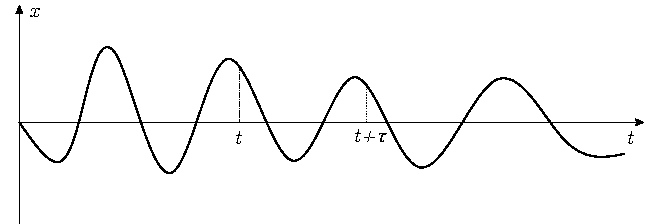
\includegraphics[]{/korelacja/korelacja.pdf}
	\captionsetup{justification=centering}
	\caption{Autokorelacja, jako korelacja wartości funkcji $x(t)$ w czasie $t$ i $t+\tau$}
	\label{fig: autocorrelationExample}
\end{figure}
\begin{equation} \label{eq: autocorrelationDef}
	R_x(\tau)=\mathrm{E}[x(t)x(t+\tau)]
\end{equation}
Funkcję cross-korelacji opiszemy analogicznie jak autokorelacji, z tą różnicą, że pod uwagę weźmiemy dwa losowe sygnały $x(t)$ i $y(t)$.
\begin{equation} \label{eq: crosscorrelationDef}
	\begin{aligned}
		R_{xy}(\tau)=\mathrm{E}[x(t)y(t+\tau)]\\	
		R_{yx}(\tau)=\mathrm{E}[y(t)x(t+\tau)]
	\end{aligned}
\end{equation}

Nie znając funkcji gęstości prawdopodobieństwa, funkcje autokorelacji  i cross-korelacji można wyznaczyć za pomocą uśredniania w czasie co opisano równaniami odpowiednio (\ref{eq: timeAveAutocorrelation}) i (\ref{eq: timeAveCrosscorrelation}). W dalszej części pracy podane zostaną inne przykłady metod wyznaczania funkcji korelacji.
\begin{equation} \label{eq: timeAveAutocorrelation}
	R_x = \frac{1}{T}\int_{0}^{T}x(t)x(t+\tau) \,dt
\end{equation}

\begin{equation} \label{eq: timeAveCrosscorrelation}
	\begin{aligned}
		R_{xy} = \frac{1}{T}\int_{0}^{T}x(t)y(t+\tau) \,dt \\
		R_{yx} = \frac{1}{T}\int_{0}^{T}y(t)x(t+\tau) \,dt 
	\end{aligned}
\end{equation}
Jedną z istotnych właściwości funkcji korelacji jest możliwość wyznaczenia jej przez splot między sygnałem $x(-t)$ i $y(t)$, co zapisano równaniem (\ref{eq: splotCorrelation}). Główną zaletą tego rozwiązania jest prostota obliczeń, ponieważ splot dwóch funkcji jest łatwy do wyznaczenia w dziedzinie częstotliwości \parencite{Brincker2015}.
\begin{equation} \label{eq: splotCorrelation}
	R_{xy}(\tau)=x(-t)*y(t)
\end{equation}
W praktyce wykonywanych jest wiele pomiarów. Załóżmy, że dla zestawu $N$ pomiarów, zmierzone odpowiedzi mogą być zestawione w wektor:
\begin{equation}
	\vect{y}(t) = \{y_1(t),y_2(t),y_3(t), \hdots ,y_N(t)\}^T
\end{equation}
Wyniki autokorelacji i cross-korelacji pomiędzy wszystkimi zmierzonymi sygnałami można zagregować i zapisać macierzowo (\ref{eq: matCorelationDef}). Na przekątnej macierzy znajdują się funkcje autokorelacji, a poza przekątną cross-korelacji.
\begin{equation} \label{eq: matCorelationDef}
	\matr{R}^T(\tau)=\mathrm{E}[\vect{y}(t)\vect{y}^T(t+\tau)]
\end{equation}
Macierzą korelacji \teng{correlation matrix} nazywa się macierz (\ref{eq: matCorelationDef}) dla $\tau=0$ co można zapisać wzorem (\ref{eq: correlationMatrixDef}).
\begin{equation} \label{eq: correlationMatrixDef}
	\matr{C}=\mathrm{E}[\vect{y}(t)\vect{y}^T(t)]=\matr{R}(0)
\end{equation}

Funkcje korelacji posiadają dwie wspomniane wcześniej właściwości kluczowe dla OMA. Po pierwsze teoretycznie pozwalają wyodrębnić wszystkie informacje na temat parametrów modalnych konstrukcji z sygnału losowego. Po drugie mogą być utożsamiane z drganiami swobodnymi, gasnącymi układu \parencite{James1995}. Oba założenia zostały wyjaśnione i udowodnione poniżej.

Założenie o reprezentacji wszystkich parametrów modalnych przez funkcje korelacji opiera się na wykorzystaniu właściwości funkcji korelacji, rozkładu normalnego oraz Centralnego Twierdzenia Granicznego \teng{central limit theorem}. Centralne Twierdzenie Graniczne mówi, że dla niezależnych zmiennych losowych $X_i$ o jednakowym rozkładzie, fluktuujących wokół wartości oczekiwanej $\mu$ i o skończonej wariancji $\sigma^2$ to wyrażenie (\ref{eq:centralLimitTheorem})
\begin{equation} \label{eq:centralLimitTheorem}
	\frac{\frac{1}{n}\sum_{i=1}^{M} X_i - \mu}{\frac{\sigma}{M}}
\end{equation}
zbiega według rozkładu do rozkładu Gaussa przy nieskończonej liczbie M.
\cite{Brincker2015} przedstawili uzasadnienie użycia tego twierdzenia w przypadku OMA w następujący sposób. Rozważmy zestaw zmiennych losowych $\{x_1,x_2,...,x_M\}$, które są niezależne i posiadają identyczny rozkład, ze średnią wartością $\mu$ i wariancją $\sigma^2$. Liniowa kombinacja tych zmiennych losowych jest dana wzorem:
\begin{equation} \label{eq:CLTsum}
	y = \sum_{i=1}^{M} a_i x_i
\end{equation}
Centralne twierdzenie graniczne mówi o tym, że dla dużej liczby zmiennych losowych $M$ rozkład $y$ jest w przybliżeniu normalny, z wartością średnią $\mu_y=\mu\sum a_i$, wariancją $\sigma_y^2=\sigma^2\sum \sigma^2$ i przy $M \xrightarrow{} \infty$ zbiega do rozkładu normalnego. Odwołując się do dynamiki budowli możemy zapisać, że odpowiedź układu $y(t)$ jest splotem siły wymuszającej $x(\tau)$ i funkcji odpowiedzi impulsowej $h(t)$ co pokazano równaniem:
\begin{equation} \label{eq:convolutionResponse}
	y(t)=\int_{-\infty}^{\infty}h(t-\tau)x(\tau) \,d\tau
\end{equation}

Dla sygnału dyskretnego z krokiem czasowym $\Delta t$ i ograniczając się jedynie do $N_m$ istotnych z punktu widzenia pamięci systemu próbek, zależność może być przedstawiona następująco:
\begin{equation}
	y(n) = \sum_{k=n-N_m}^{n} h(n-k)x(k)\Delta t
\end{equation}
Można zauważyć, że dla wymuszenia szumem białym odpowiedź dynamiczna $y(n)$ jest sumą, którą można przedstawić wzorem (\ref{eq:CLTsum}), gdzie poszczególne składniki obciążenia $x(k)$ nie muszą mieć rozkładu normalnego, ale ostateczna odpowiedź będzie mieć rozkład Gaussa. Wynika to wprost z Centralnego Twierdzenia Granicznego. Warto nadmienić, że założenie o wymuszeniu białym szumem zapewnia nam niezależność składników obciążenia $x(k)$. 

Bazując na powyższym, w OMA zwykle zakładamy, że mierzone sygnały posiadają wartość średnią równą zero oraz są Gaussowskie \teng{Gaussian signals} lub bliskie Gaussowskim \parencite{Brincker2015}. Przypomnijmy, że jednowymiarowa funkcja gęstości prawdopodobieństwa rozkładu normalnego dana jest wzorem:
\begin{equation}
	p(x) = \frac{1}{\sqrt{2\pi\sigma^2}}e^{-\frac{(x-\mu)^2}{2\sigma^2}}
\end{equation}
, a przyjmując dodatkowo wartość średnią równą
zero wzór można wyrazić następująco:
\begin{equation} \label{eq:normalDensZeroMean}
	p(x) = \frac{1}{\sqrt{2\pi\sigma^2}}e^{-\frac{x^2}{2\sigma^2}}
\end{equation}
Dla wektora losowego, zawierającego zmienne losowe o zerowej wartości średniej $\vect{x}^T=\{x_1,x_2,x_3,\hdots,x_M\}$, funkcja gęstości prawdopodobieństwa może być zapisana jako:
\begin{equation}\label{eq: normalDistributionCorr}
	p(x) = \frac{1}{(2\pi)^\frac{M}{2} \matr{|C|}}e^{\vect{x}^T\matr{C}^{-1}\vect{x}/2}
\end{equation}
gdzie $|\matr{C}|$ jest wyznacznikiem macierzy korelacji (\ref{eq: correlationMatrixDef}). Podstawowym wnioskiem wynikającym z tej zależności jest to, że jednowymiarowy rozkład Gaussa może być opisany za pomocą średniej wartości, odchylenia standardowego i w przypadku wielowymiarowych danych o zerowej wartości średniej, jedynie przez przez macierz korelacji (\ref{eq: normalDistributionCorr}).

Aby wytłumaczyć dlaczego funkcje korelacji w OMA mogą być odpowiednikiem funkcji odpowiedzi impulsowej (IRF), a funkcje gęstości widmowej odpowiednikami funkcji odpowiedzi częstotliwościowej (FRF) przytoczmy wymagane definicje i zależności z dynamiki budowli. Szczegółowe wyprowadzenia i objaśnienia znajdują się między innymi w pracach \parencite{Brincker2015,Rainieri2014,Chopra2012a,Ewins2000}. Funkcja odpowiedzi impulsowej układu, zwykle oznaczone jako $h(t)$ jest odpowiedzią układu poddanego wymuszeniu przez impulsową siłę, o bardzo krótkim czasie działania, w chwili czasowej $t=0$. Matematycznie impulsową siłę opisuje funkcja nazywaną deltą Diraca $\delta(t)$. Dla systemów liniowych i czasowo niezależnych, jeżeli przesunięta w czasie zostanie chwila przyłożenia impulsu o $\tau$, to otrzymamy odpowiedź $y(t)$, która będzie również przesunięta w czasie o $\tau$. Z definicji wiemy, że impuls jest iloczynem intensywności obciążenia i czasu jego działania. Rozważmy ciągłe obciążenie oznaczone jako $x(t)$, które jest superpozycją potoku impulsów o zmiennej amplitudzie, ale o równie krótkich czasach trwania. W takim przypadku impuls siły od czasu $\tau$ do $\tau+d\tau$ obliczamy jako $x(\tau)d\tau$, a odpowiedź układu jako $h(t-\tau)x(\tau)d\tau$. Układ jest liniowy a więc obowiązuje zasada superpozycji. Wynika z tego, że suma wpływu całego obciążenia może być wyznaczona jako suma wszystkich składowych odpowiedzio i opisana całką Duhamel'a jako (\ref{eq: duhamelIntegralIRF}) oraz w postaci splotu (\ref{eq: convolutionIntegralIRF}) miedzy funkcją IRF $h(t)$ i wymuszeniem $x(t)$.
\begin{equation} \label{eq: duhamelIntegralIRF}
	y(t)=\int_{-\infty}^{\infty} h(t-\tau)x(\tau)d\tau
\end{equation}
\begin{equation} \label{eq: convolutionIntegralIRF}
	y(t)=h(t)*x(t)
\end{equation}
Funkcję IRF można wyznaczyć wykonując przekształcenie Laplace'a równania ruchu przedstwaionego równaniem (\ref{eq: mot_und}). Dla przejrzystości przytoczono je poniżej (\ref{eq: motionIRF}), dla układu z jednym stopniem swobody, wymuszenia deltą Diraca i podstawiając w miejsce odpowiedzi układu funkcję IRF:
\begin{equation} \label{eq: motionIRF}
	m\ddot{h}(t)+c\dot{h}(t)+kh(t)=\delta(t)
\end{equation}
Wykonując transformatę Laplace'a obu stron otrzymamy:
\begin{equation} \label{eq: laplaceTransofrmMOVEQ}
	(ms^2+cs+k)H(s)=1
\end{equation}
Wykorzystując właściwości transformaty i przekształcając odpowiednio równanie (\ref{eq: laplaceTransofrmMOVEQ}) otrzymamy formułę (\ref{eq: laplaceTransofrmMOVEQ2}). Na jej podstawie można wprost wyznaczyć funkcje IRF podaną równaniem (\ref{eq: IRFfunction}).
\begin{equation} \label{eq: laplaceTransofrmMOVEQ2}
	H(s) = \frac{1}{m(s-\lambda)(s-\lambda^*)}
\end{equation}
\begin{equation} \label{eq: IRFfunction}
	h(t)=\frac{1}{m}\frac{e^{\lambda t}-e^{\lambda^*t}}{\lambda-\lambda^*}
\end{equation}



Z kolei funkcja FRF w sensie fizycznym reprezentuje amplitudę i przesunięcie fazowe drgań ustalonych systemu SDOF, poddanego wymuszeniu harmonicznemu o jednostkowej amplitudzie i częstotliwości $\omega_d$. Matematycznie FRF $H(\omega)$ można opisać również jako transformatę Laplace'a z IRF obliczoną dla urojonej współrzędnej $s=i\omega$ (\ref{eq: laplaceTransofrmMOVEQ2}) i zapisać następująco:
\begin{equation} \label{eq: FRFfunction}
	H(\omega)=\frac{1}{m(i\omega-\lambda)(i\omega-\lambda^*)}
\end{equation}
Podobnie jak IRF, FRF łączy wymuszenie z odpowiedzią układu. Jeśli równanie ruchu (\ref{eq: mot_und}) stronami przekształcimy transformatą Fouriera to otrzymamy:
\begin{equation} \label{eq: FRF_moteq}
	(m(i\omega)^2+ci\omega + k)Y(\omega)=X(\omega)
\end{equation}
Szczegółowe rozwiązanie za pomocą reprezentacji biegunów układu można znaleźć w literaturze \parencite{Brincker2015}. Ostatecznie otrzymujemy:
\begin{equation} 
	m(i\omega-\lambda)(i\omega-\lambda^*)Y(\omega)=X(\omega)
\end{equation}
Po przekształceniu wyraźnie widać relację pomiędzy odpowiedzią, a wymuszeniem układu za pośrednictwem FRF:
\begin{equation} \label{eq: FRF_final}
	Y(\omega)=\frac{1}{m(i\omega-\lambda)(i\omega-\lambda^*)}X(\omega)=H(\omega)X(\omega)
\end{equation}
gdzie $X(\omega)$ i $Y(\omega)$ są odpowiednio transformatami Fouriera wymuszenia $x(t)$ i odpowiedzi $y(t)$ układu. Porównując równania (\ref{eq: FRF_moteq})(\ref{eq: FRF_final}) łatwo można zauważyć że FRF zawiera w sobie informację na temat bezwładności, tłumienia i sztywności układu.




Zarówno IRF jak i FRF można uogólnić do układów MDOF o $N$ stopniach swobody. Zapis zależności wymuszenie-odpowiedź dla układu MIMO (wiele-wejść-wiele-wyjść) przedstawiono dla dziedziny czasu (\ref{eq: mimoIRFyx}) i częstotliwości (\ref{eq: mimoFRFyx}).

\begin{equation} \label{eq: mimoIRFyx}
	\vect{y}(t)=\matr{H}(t)*\vect{x}(t)
\end{equation}
\begin{equation} \label{eq: mimoFRFyx}
	\vect{\tilde{y}}(\omega)=\matr{\tilde{H}}(i\omega)\vect{\tilde{x}}(\omega)
\end{equation}
gdzie $\matr{H}(t)$ jest macierzą zawierającą funkcje IRF, $\vect{x}(t)$ jest wektorem sił wymuszających, $\vect{\tilde{y}}(\omega)$ i $\vect{\tilde{x}}(\omega)$ są transformatami Fouriera odpowiednio $\vect{x}(t)$ i $\vect{y}(t)$, a $\matr{\tilde{H}}(i\omega)$ jest macierzą FRF. Wyrażenia na odpowiednio IRF $\matr{H}(t)$ i FRF $\matr{\tilde{H}}(i\omega)$ podano poniżej.
\begin{equation} \label{eq: IRFmimo}
	\matr{H}(t)=\sum_{n=1}^{N}(\vect{A}_n e^{\lambda_n t} + \vect{A}_n^* e^{\lambda_n t})
\end{equation} 
\begin{equation} \label{eq: FRFmimo}
	\matr{\tilde{H}}(i\omega)=\sum_{n=1}^{N}(\frac{\vect{A}_n}{i\omega-\lambda_n} + \frac{\vect{A}_n^*}{i\omega-\lambda_n^*})
\end{equation}
gdzie $\vect{A}_n=Q_n \vect{\psi}_n\vect{\psi}_n^T$, $\vect{\psi}_n$ to n-ta postać drgań własnych, $Q_n$ to współczynnik skalujący mody, a $\lambda_n=\sigma_n+i\omega_{d,n}$ jest n-tym biegunem układu zawierającym informacje na temat częstotliwości drgań własnych tłumionych $f_{d,n}=\omega_{d,n}/(2\pi)$ i liczby tłumienia $\xi_r=-\sigma_n/\sqrt{\sigma_n^2+\omega_{d,n}^2}$ n-tego moda.






Gęstość widmowa jest kolejnym kluczowym pojęciem potrzebnym do pełnego zrozumieniu znaczenia funkcji korelacji dla OMA. Gęstość widmowa \teng{auto spectral density} dla przebiegu czasowego $x(t)$ jest zdefiniowana jako transformata Fouriera z funkcji korelacji $R_x(\tau)$ \ref{eq: spectralDensity}. Istnieje również zależność odwrotna, w której odwrotną transformata Fouriera z gęstości widmowej pozwala otrzymać funkcję korelacji \ref{eq: correlationInversSpectralDensity}. Początkowy wyraz funkcji korelacji $R_x(0)$ jest reprezentacją twierdzenia Parsevela i pozwala stwierdzić, że gęstość widmowa pokazuje rozkład energii w funkcji częstotliwości. Stąd gęstość widmową nazywa się również zamiennie gęstością widmową mocy \teng{power spectral density} (PSD) \parencite{Brincker2015}.
\begin{equation} \label{eq: spectralDensity}
	G_x(\omega) = \frac{1}{2\pi}\int_{-\infty}^{\infty}R_x(\tau)e^{-i\omega\tau}\,d\tau
\end{equation}
\begin{equation} \label{eq: correlationInversSpectralDensity}
	R_x(\omega) = \int_{-\infty}^{\infty}G_x(\omega)e^{i\omega\tau}\,d\omega
\end{equation}
Podobnie zdefiniować można gęstość widmową pomiędzy dwoma sygnałami $x(t)$ i $y(t)$ \teng{cross spectral density}, jako przekształcenie Fouriera funkcji cross-korelacji $R_{xy}(t)$. 

\begin{equation} \label{eq: crossspectralDensity}
	G_{xy}(\omega) = \frac{1}{2\pi}\int_{-\infty}^{\infty}R_{xy}(\tau)e^{-i\omega\tau}\,d\tau
\end{equation}
\begin{equation} \label{eq: crosscorrelationInversSpectralDensity}
	R_{xy}(\omega) = \int_{-\infty}^{\infty}G_{xy}(\omega)e^{i\omega\tau}\,d\omega
\end{equation}
Wykorzystanie właściwości splotu funkcji korelacji (\ref{eq: splotCorrelation}) i  splotu\footnote{Transformata Fouriera splotu dwóch funkcji w dziedzinie czasu $h(t)$ i $g(t)$ jest równa iloczynowi transformat Fouriera każdej z funkcji osobno. Innymi słowy transformacie Fouriera wyrażenia $h(t)*g(t)$ odpowiada iloczyn $H_k G_k$, gdzie: $H_k$ - transformata Fouriera funkcji $h(t)$, $G_k$ - transformata Fouriera funkcji $g(t)$.} oraz symetrii Hermitowskiej\footnote{Jeżeli $H(\omega)$ jest transformatą Fouriera rzeczywistej funkcji $h(t)$, to prawdziwe jest równanie $H(\omega)=H^*(-\omega)$. Równanie to jest nazywane symetrią Hermitowską \parencite{Boashash2015}.} transformaty Fouriera pozwala uzyskać następującą właściwość gęstości widmowej (\ref{eq: specDensSplot}). Należy nadmienić, że zależność ta będzie spełniona przy założeniu okresowego (lub bardzo długiego) sygnału \parencite{Brincker2015}.
\begin{equation} \label{eq: specDensSplot}
	G_{xy}(\omega) = X^*(\omega)Y(\omega)
\end{equation}


Rozważamy ponownie układ SISO o odpowiedzi $y(t)$ przy wzbudzeniu $x(t)$: $y(t)=x(t)*h(t)$ (\ref{eq: convolutionIntegralIRF}). Wykorzystując równanie (\ref{eq: specDensSplot}) zapiszemy równanie na gęstość widmową odpowiedzi:
\begin{equation} \label{g}
	G_{y}(\omega) = Y^*(\omega)Y(\omega)
\end{equation}
Wykorzystując transformatę Fouriera oraz przemienność i łączność splotu zapisać można następujące równanie pokazujące zależność pomiędzy gęstością widmową odpowiedzi i wymuszenia układu.
\begin{equation} \label{eq: sisofundamentaltheorem}
	G_{y}(\omega) = G_x(\omega)|H^*(i\omega)|^2
\end{equation}
Równanie (\ref{eq: sisofundamentaltheorem}) jest nazywane twierdzeniem podstawowym \teng{fundamental theorem} metody OMA. Dla układu MIMO twierdzenie to przyjmuje następującą formę w dziedzinie częstotliwości:
\begin{equation} \label{eq: matrixoutputspectraldensity}
	\begin{split}
		\matr{G}_{y}(\omega) &=\matr{\tilde{H}}^*(i\omega)\matr{G}_x(\omega)\matr{\tilde{H}}^T(i\omega)\\
		&=\matr{\tilde{H}}^*(i\omega)\matr{G}_x(\omega)\matr{\tilde{H}}^T(i\omega)
	\end{split}
\end{equation}
z kolei w dziedzinie czasu odpowiadająca macierz korelacji przedstawia się następująco:
\begin{equation} \label{eq: matrixoutputcorrelation}
	\matr{R}_y(\tau)=\matr{H}(-\tau)*\matr{R}_x(\tau)*\matr{H}^T(\tau)
\end{equation}

Jak już wielokrotnie wspomniano, w OMA zakłada się wymuszenie Gaussowskim, stacjonarnym szumem białym o zerowej wartości średniej. Podstawowym efektem tego założenia wymuszenia $x(t)$ w postaci białego szumu jest brak korelacji pomiędzy wymuszeniem w chwili $t$ i w chwili $t+\tau$. Wyjątkiem jest przypadek $\tau=0$. Stąd sygnał posiada zerową wartość średnią, a funkcja korelacji jest deltą Diraca co zapiszemy:
\begin{equation}
	R_x(\tau)=\mathrm{E}[x(t)x(t+\tau)] = 2\pi G_{x0} \delta(\tau)
\end{equation} 
gdzie $G_{x0}$ jest współczynnikiem skalującym. Zakładając dalej, że biały szum działa jedynie w ograniczonym spektrum od $0$ do $B$, a $\sigma_x^2$ to niezmiennie wariancja sygnału, otrzymamy przekształconą wersję () funkcji korelacji. Na jej podstawie można stwierdzić, że PSD wymuszenia (będąca transformatą Fouriera funkcji korelacji) jest wartością stałą\footnote{Transformata Fouriera delty Diraca jest równa jedności: $\int_{-\infty}^{\infty} \delta(t) e^{i\omega t}\,dt = e^{-i\omega\times 0}=1$ \parencite{Zielinski2002}} .
\begin{equation} \label{eq: whitenoisecorrelationSISO}
	R_x(\tau)=2\pi \frac{\sigma_x^2}{2B} \delta(\tau)
\end{equation} 

Chcąc rozwinąć tę zależność do układu MIMO załóżmy sygnały wymuszenia $x_1(t)$ i $x_2(t)$ jako szumy białe. Sformułowanie macierzy korelacji z wykorzystaniem równania (\ref{eq: whitenoisecorrelationSISO}) prowadzi do następującej zależności:
\begin{equation} \label{eq: whitenoisecorrelationMIMO}
	\matr{R}_x(\tau)=\mathrm{E}[\vect{x}(t)\vect{x}^T(t+\tau)]=2\pi \frac{\delta(\tau)}{2B}\matr{C}
\end{equation} 
gdzie $\matr{C}$ jest macierzą kowariancji sygnałów. Macierz gęstości widmowej sygnałów wymuszenia szumem białym ma postać:
\begin{equation} \label{eq: spectraldensitymatrixWHITENOISE}
	\matr{G}_x(\omega)=\begin{cases}
		\frac{\matr{C}}{2B}, & 0\le\omega\le B\\
		0, & \omega>B
	\end{cases}
\end{equation} 


Podsumowując powyższy ciąg myślowy możliwa jest dekompozycja równania (\ref{eq: matrixoutputcorrelation}) w dziedzinie czasu i równania (\ref{eq: matrixoutputspectraldensity}) w dziedzinie częstotliwości. Dekompozycję w dziedzinie czasu przeprowadzili po raz pierwszy \cite{James1993,James1995}. Z kolei dekompozycję w dziedzinie częstotliwości przedstawili \cite{Brincker2000,Brincker2001a}. W powyższych pracach przedstawiono pełny tok postępowania. Poniżej przytoczono rezultaty końcowe w postaci opisu macierzy korelacji sygnałów odpowiedzi układu (\ref{eq: decomposedRx}) i macierzy korelacji gęstości widmowej odpowiedzi (\ref{eq: decomposedGx}).

\begin{equation} \label{eq: decomposedRx}
	\matr{R}_y(\tau)=\begin{cases}
		\sum_{n=1}^{N} (\vect{\phi_n}{\vect{\gamma}_n}^Te^{\lambda_n \tau} + \vect{\phi_n}^*{\vect{\gamma}_n}^He^{\lambda_n^* \tau}), & \tau\ge 0\\
		\sum_{n=1}^{N} (\vect{\gamma_n}{\vect{\phi}_n}^Te^{-\lambda_n |\tau|} + \vect{\gamma_n}^*{\vect{\phi}_n}^He^{-\lambda_n^* |\tau|}), & \tau< 0.
	\end{cases}
\end{equation} 

\begin{equation} \label{eq: decomposedGx}
	\matr{G}_y(\omega)=\sum_{n=1}^{N}\frac{\vect{\phi_n}{\vect{\gamma}_n}^T}{i\omega-\lambda_r}+\frac{\vect{\phi_n}^*{\vect{\gamma}_n}^H}{i\omega-\lambda_r^*}+\frac{{\vect{\gamma}_n}\vect{\phi_n}^T}{-i\omega-\lambda_r}+\frac{{\vect{\gamma}_n}^*\vect{\phi_n}^H}{-i\omega-\lambda_r^*}
\end{equation} 


gdzie oznaczenia przyjęto jak w równaniach (\ref{eq: IRFmimo}) i (\ref{eq: FRFmimo}), a $\vect{\gamma}_n$ oznacza wektor referencyjny związany z n-tym modem. Wektor ten zależny jest od wszystkich parametrów modalnych systemu oraz lokalizacji i macierzy korelacji wymuszeń \parencite{Rainieri2014, Peeters2000}. 

Równanie (\ref{eq: decomposedRx}) pokazuje, że funkcje korelacji odpowiedzi mogą być wyrażone za pomocą sumy zespolonych funkcji eksponencjalnych. \cite{SHEN2003} wskazują na podobieństwo jego formy do równania (\ref{eq: IRFmimo}). \cite{Kennedy1995}, w swojej kluczowej dla metody NExT pracy, rozwinęli to równanie do postaci ukazującej funkcję korelacji jako sumę zanikających sinusoid, o charakterystyce takiej samej jak w przypadku IRF. Podsumowując, funkcje korelacji mogą być użyte jako funkcje odpowiedzi impulsowej (IRF) w metodach TD identyfikacji parametrów modalnych.


\subsection{Eigenystem Realization Algorithm}
Metoda ERA została opracowana w latach 80' XX w. przez naukowców z NASA Langley Research Center: Richarda Pappa i Jer-Nan Juang'a. Przedstawili oni koncept identyfikacji modalnej i redukcji modelu układu dynamicznego na podstawie danych pomiarowych. Nowością, którą wprowadzili autorzy było połączenie pojęć z teorii kontroli i algorytmu rozkładu względem wartości osobliwych. Fundamentalne prace opisujące metodą zostały opisane w \parencite{Pappa1985,Juang1985,Juang1988,Juang1994}. Algorytm ERA był wielokrotnie testowany, na przykaład pod względem odporności na zaszumienie danych pomiarowych \parencite{Juang1986, Li2011}. Spośród polskich autorów, szczegółowy opis metody zawarli w swoich pracach \cite{Szafranski2013} i \cite{Dudek2008}.

\subsubsection{Liniowy model dynamiczny w przestrzeni stanów}
Model przestrzeni stanów\footnote{Według \cite{Kaczorek2016} stanem układu nazywamy zbiór liniowo niezależnych wielkości $x_1, x_2, x_3,\dots,x_n$ określających w pełni skutki przeszłych oddziaływań $(t<t_0)$ na układ, który jest wystarczający do wyznaczenie przebiegów chwilowych dowolnych wielkości w tym układzie dla $t>t_0$, gdy znane są wymuszenia i parametry obwodu. Wielkości $x_1, x_2, x_3,\dots,x_n$ nazywa się zmiennymi stanu, a wektor $\vect{x}=[x_1, x_2, x_3,\dots,x_n]$ wektorem stanu tego obwodu.} \teng{state-space model} używany jest do przekształcenia równania różniczkowego drugiego rzędu (\ref{eq: mot_dam}), do dwóch równań rzędu pierwszego.     Dla przejrzystości macierzowe równanie ruchu przytoczono ponownie poniżej:
\begin{equation}
	\vect{M} \vect{\ddot{x}}(t) +\vect{C} \vect{\dot{x}}(t)+ \vect{Kx}(t) = \vect{F}(t)
\end{equation}
gdzie: $\vect{M}$, $\vect{C}$, $\vect{K}$ to odpowiednio macierze mas, tłumienia i sztywności, $\vect{x}(t)$ jest wektorem przemieszczenia, a $\vect{F}(t)$ jest wektorem wymuszenia. 
Wektor wymuszenia można poddać faktoryzacji do macierzy $\vect{\bar{B}}$ oraz wektora $\vect{u}(t)$ (\ref{eq: }). Macierz $\vect{\bar{B}}$ opisuje lokalizację punków wymuszenia, a wektor $\vect{u}(t)$ intensywność tego wymuszenia w funkcji czasu.
\begin{equation}
	\vect{F}(t) = \vect{\bar{B}}\vect{u}(t)
\end{equation} 
Macierzowe równanie ruchu może być więc przekształcone następująco:
\begin{equation} \label{eq: STATEmanipulated_mot_eq}
	\vect{\ddot{x}}(t) +\vect{M}^{-1} \vect{C} \vect{\dot{x}}(t)+ \vect{M}^{-1}\vect{Kx}(t) = \vect{M}^{-1}\vect{\bar{B}}\vect{u}(t)
\end{equation}
Zdefiniujmy wektor stanu jako:
\begin{equation} \label{eq: stateVector}
	\vect{s}(t) = \begin{Bmatrix}
		\vect{\dot{x}}(t) \\
		\vect{x}(t)
	\end{Bmatrix}
\end{equation}
Liczba komponentów tworzących wektor stanu jest nazywana rzędem modelu. Podstawiając go do równania (\ref{eq: STATEmanipulated_mot_eq}) dodatkowo wykorzystując oczywistą równość $\vect{M}\vect{\dot{x}}(t)=\vect{M}\vect{\dot{x}}(t)$ otrzymamy:
\begin{equation}
	\vect{\dot{s}}(t) = 
	\begin{bmatrix}
		-\vect{M}^{-1}\vect{C} & -\vect{M}^{-1}\vect{K} \\
		\vect{I} & \vect{0}
	\end{bmatrix} \vect{s}(t) + 
	\begin{bmatrix}
		-\vect{M}^{-1}\vect{\bar{B}} \\
		\vect{0}
	\end{bmatrix} \vect{u}(t)
\end{equation}
Stąd możemy zdefiniować następujące macierze: $\vect{A}_c$ i $\vect{B}_c$:
\begin{equation}
	\vect{A}_c = 
	\begin{bmatrix}
		-\vect{M}^{-1}\vect{C} & -\vect{M}^{-1}\vect{K} \\
		\vect{I} & \vect{0}
	\end{bmatrix} 
\end{equation}
\begin{equation}
	\vect{B}_c = 
	\begin{bmatrix}
		-\vect{M}^{-1}\vect{\bar{B}} \\
		\vect{0}
	\end{bmatrix}\phantom{\qquad\qquad\quad}
\end{equation}
Dzięki tak sformułowanym elementom zapiszmy równanie stanu \teng{state equation} następująco:
\begin{equation} \label{eq: stateEquation}
	\vect{\dot{s}}(t)= \vect{A}_c\vect{s}(t)+\vect{B}_c\vect{u}(t)
\end{equation}
W równaniu (\ref{eq: stateEquation}) $\vect{s}(t)$ jest wektorem stanu (\ref{eq: stateVector}), czyli zestawem wielkości opisujących w sposób jednoznaczny stan modelowanego układu, a $\vect{u}(t)$ jest wektorem wejścia (sterowania) i opisuje sygnał wejściowy. Macierze $\vect{A}_c$ i $\vect{B}_c$, nazywane są odpowiednio macierzą stanu (systemu) \teng{state matrix} i macierzą wejścia \teng{input influecne matrix}. Są to macierze stałych współczynników, które odwzorowują modelowany układ dynamiczny i parametry elementów tworzących ten układ.

Drugim równaniem pozwalającym na stworzenie modelu w przestrzeni stanów jest równanie obserwacji \teng{observation equation} lub inaczej równanie wyjścia. W ogólności ma ono postać:
\begin{equation} \label{eq: observationEquationCont}
	\vect{y}(t) = \vect{C_a}\vect{\ddot{x}}(t) + \vect{C_v}\vect{\dot{x}}(t) +\vect{C_d}\vect{x}(t)
\end{equation}
gdzie: $\vect{y}(t)$ jest wektorem mierzonej odpowiedzi w $m$ punktach pomiarowych, a $\vect{\ddot{x}}(t)$, $\vect{\dot{x}}(t)$ i $\vect{x}(t)$ to odpowiednio mierzone przyspieszenia, prędkości i przemieszczenia w danych $m$ punktach. Z kolei macierze $\vect{C_a}$, $\vect{C_v}$ i $\vect{C_d}$ określają lokalizację mierzonych, odpowiadających im przyspieszeń, prędkości i przemieszczeń. Należy zaznaczyć, że rzeczywista konstrukcja składa się z nieskończonej liczby stopni swobody. Nawet w przypadku dyskretyzacji do układu MDOF, jak to ma miejsce w przypadku obliczeń numerycznych, liczba stopni swobody jest ogromna. Z tego względu, w trakcie pomiarów znacznie redukuje się liczbę mierzonych stopni swobody właśnie do $m$. Podstawiając równanie (\ref{eq: STATEmanipulated_mot_eq}) do (\ref{eq: observationEquationCont}), po przekształceniach można otrzymać następujące równanie obserwacji:
\begin{equation} \label{eq: observationEquation}
	\vect{y}(t) = \vect{C}_c\vect{s}(t)+\vect{D}_c\vect{u}(t)
\end{equation}
w którym:
\begin{equation}
	\vect{C}_c = 
	\begin{bmatrix} 
		\vect{C}_v-\vect{C}_a\vect{M}^{-1}\vect{C}  &  \vect{C}_d-\vect{C}_a\vect{M}^{-1}\vect{K}
	\end{bmatrix}
\end{equation}
\begin{equation}
	\vect{D}_c = \vect{C}_a\vect{M}^{-1}\vect{\bar{B}} \phantom{\qquad\qquad\qquad\qquad\qquad\quad.}
\end{equation}
Macierz $\vect{C}_c$ jest nazywana macierzą wyjścia \teng{output influence matrix}, a $\vect{D}_c$ macierzą przenoszenia lub transmisyjną \teng{direct transmission matrix}. Równania stanu (\ref{eq: stateEquation}) i obserwacji (\ref{eq: observationEquation}) łącznie tworzą ciągły, deterministyczny model przestrzeni stanów:
\begin{equation} \label{eq: con_state_space_model}
	\begin{aligned}
		\vect{\dot{s}}(t)= \vect{A}_c\vect{s}(t)+\vect{B}_c\vect{u}(t) \\
		\vect{y}(t) = \vect{C}_c\vect{s}(t)+\vect{D}_c\vect{u}(t)
	\end{aligned}
\end{equation}

Wielkości mierzone w trakcie eksperymentu są próbkowane jedynie w dyskretnych chwilach czasowych. W takim razie, naturalnym dla rzeczywistych zastosowań jest przekształcenie modelu ciągłego przestrzeni stanów w model dyskretny. Zakładając stały czas próbkowania równy $\Delta t$, równania ciągłe mogą być zdyskretyzowane i rozwiązane jedynie w chwilach czasowych $t_k=k\Delta t$ dla $k\in N$. Dla poprawności zapisu dyskretnego, wymagane jest założenie o stałych wartościach elementów wektora wejścia $\vect{u}(t)$ w trakcie pojedynczego kroku czasowego, tj. $\vect{u}(t)=\vect{u}_k$ dla $t \in [k\Delta t, (k+1)\Delta t]$. Przy spełnieniu powyższych założeń możemy zapisać dyskretny model przestrzeni stanów:
\begin{equation} \label{eq: dis_state_space_model}
	\begin{aligned}
		\vect{\dot{s}}_{k+1}= \vect{A}\vect{s}_k+\vect{B}\vect{u}_k \\
		\vect{y}_k = \vect{C}\vect{s}_k+\vect{D}\vect{u}_k
	\end{aligned}
\end{equation}
gdzie macierze $\vect{A}$, $\vect{B}$, $\vect{C}$, $\vect{D}$ są odpowiednio macierzami stanu, wejścia, wyjścia i przenoszenia dla dyskretnego modelu przestrzeni stanów.

\subsubsection{Odpowiedź impulsowa w przestrzeni stanów}
Przyjmijmy układ dynamiczny opisany równaniem (\ref{eq: dis_state_space_model}), w którym $\vect{s}_k$ - jest n-wymiarowym wektorem stan, $\vect{u}_k$ - m-wymiarowym wektorem sterowania, a $\vect{y}_k$ - p-wymiarowym wektorem obserwacji. Parametry Markova takiego systemu $\vect{G}_k$ można zdefiniować następująco \parencite{Schutter2000}:
\begin{equation} \label{eq: markovParameters}
	\vect{G}_k= \begin{cases}
		\vect{D}, & \text{dla }k=0 \\
		\vect{C}\vect{A}^{k-1}\vect{B}, & \text{dla }k=1,2, \dots
	\end{cases}
\end{equation}
Jeżeli spełnione jest równanie (\ref{eq: markovParameters}) to zestaw macierzy $\vect{A}$, $\vect{B}$, $\vect{C}$, $\vect{D}$ jest realizacją łańcucha $G(k)\; \text{dla } k=1,2\dots,\infty$. Realizację nazywa się minimalną, kiedy rząd modelu jest minimalny (\ref{eq: stateVector}).

Zakładając warunek początkowy $\vect{s}(0)=\vect{0}$ i wymuszenie wszystkich punktów układu jednostkowym impulsem w postaci:
\begin{equation}
	\delta_k = \begin{cases}
		1, & \text{dla }k=0 \\
		0, & \text{dla } k>0 
	\end{cases}
\end{equation}
otrzymamy odpowiedź układu postaci:
\begin{equation} \label{eq: impulseInputLTI}
	\vect{Y}_k= \begin{cases}
		\vect{D}, & \text{dla }k=0 \\
		\vect{C}\vect{A}^{k-1}\vect{B}, & \text{dla }k=1,2, \dots
	\end{cases}
\end{equation}
Równanie (\ref{eq: impulseInputLTI}) nazywa się odpowiedzią impulsową układu. Można zauważyć, że elementy sekwencji parametrów Markova odpowiadają wprost elementom odpowiedzi impulsowej układu \parencite{Phan1991}.
W przypadku identyfikacji modalnej rzeczywistej konstrukcji wyznaczenie macierzy opisujących układ jest celem. Dysponując pomierzonym sygnałem odpowiedzi swobodnej (wzbudzonej impulsem) możliwe jest sformułowanie parametrów Markova i poszukiwanie rozwiązania w postaci macierzy układu. W przypadku OMA odpowiedź impulsowa układu może być zastąpiona funkcjami korelacji co udowodniono w (\ref{sect: correlationFunction}).
Niezależnie od źródła danych, sygnały można złożyć w parametry Markova w identyczny sposób. W dalszej części wywodu elementy algorytmu ERA opisywane będą w sposób tradycyjny, operując na sygnale z odpowiedzi swobodnej układu. 

Załóżmy, że $y_k^i$ jest odpowiedzią konstrukcji w chwili czasowej $k\Delta t$, zmierzoną w punkcie pomiarowym $n$, jednym z wszystkich $m$ punktów pomiarowych. Parametry Markova $\vect{Y}_k$ zdefiniujemy zestawiając odpowiedź układu z wszystkich punktów pomiarowych dla danej chwili czasowej $k\Delta t$:
\begin{equation}
	\vect{Y}_k = \begin{Bmatrix}
		y_k^1 \\ y_k^2 \\ y_k^3 \\ \vdots \\ y_k^m 
	\end{Bmatrix},
	\qquad \text{dla } k=1,2,3,\dots
\end{equation}
\subsubsection{Sformułowanie macierzy Hankela} \label{section: hankelMatrix}
Algorytm metody ERA rozpoczyna się od sformułowania uogólnionej, blokowej\footnote{Macierz blokową można opisać jako macierz złożoną z innych macierzy. Na przykład mając 4 macierze $N \times N$: $\vect{A}_1$, $\vect{A}_2$, $\vect{A}_3$, $\vect{A}_4$, można sformułować macierz $2N\times2N$ postaci $\vect{A}=\big[\begin{smallmatrix}
		\vect{A}_1 & \vect{A}_2\\
		\vect{A}_3 & \vect{A}_4
	\end{smallmatrix}\big]$, która posiada dwa blokowe wiersze i dwie blokowe kolumny.
}  
macierzy Hankela\footnote{W ogólności macierzą Hankela nazywamy taką macierz $\vect{A}$ o wymiarach $r\times s$, że spełniona jest równość: $\vect{A_{r+1,s-1}}=\vect{A_{r-1,s+1}}$ 
} 
dyskretnego układu dynamicznego $\vect{H}$ o wymiarach $r\times s$. Wymiary $r$ i $s$ nazywane są parametrami projektowymi \parencite{Szafranski2013} i oznaczają: $r$ - liczbę blokowych wierszy, $s$ - liczbę blokowych kolumn macierzy Hankela. Jeżeli spełnione są warunki $s>n$ i $r>n$ to właściwością macierzy Hankela jest to, że w przypadku pomiarów pozbawionych szumów rząd macierzy Hankela jest równy rzędowi systemu oraz dwukrotnej liczbie modów systemu.
\begin{equation} \label{eq: genericHankelMatrix}
	\begin{split}
		\vect{H}_{k-1}&=\begin{bmatrix}
			\vect{Y}_k		&	\vect{Y}_{k+1} 	& \dots	& \vect{Y}_{k+s-1} \\
			\vect{Y}_{k+1}	&	\vect{Y}_{k+2}	& \dots	& \vect{Y}_{1+k+s-1} \\
			\vect{Y}_{k+2}	&	\vect{Y}_{k+3} 	& \dots	& \vect{Y}_{2+k+s-1} \\	
			\vdots			&	\vdots			& \ddots & \vdots\\
			\vect{Y}_{r-1+k}	&	\vect{Y}_{r-1+k+1} 	& \dots	& \vect{Y}_{r-1+k+s-1} 	
		\end{bmatrix} \\ 
		&= \begin{bmatrix}
			\vect{C}\vect{A}^{k-1}\vect{B}	&	\vect{C}\vect{A}^{k}\vect{B} 	& \dots	 & \vect{C}\vect{A}^{k+s-2}\vect{B} \\
			\vect{C}\vect{A}^{k}\vect{B}	&	\vect{C}\vect{A}^{k+1}\vect{B} 	& \dots	 & \vect{C}\vect{A}^{k+1+s-2}\vect{B} \\
			\vect{C}\vect{A}^{k+1}\vect{B}	&	\vect{C}\vect{A}^{k+2}\vect{B} 	& \dots	 & \vect{C}\vect{A}^{k+3+s-2}\vect{B} \\	
			\vdots							&	\vdots							& \ddots & \vdots\\
			\vect{C}\vect{A}^{r-2+k}\vect{B}	&	\vect{C}\vect{A}^{r-2+k+1}\vect{B} 	& \dots	 & \vect{C}\vect{A}^{r+k+s-3}\vect{B} 	
		\end{bmatrix}\in \mathcal{R}^{rm\times sp}\\
		&= \vect{P}_r \vect{A}^{k-1}\vect{Q}_s\qquad \text{dla } k\ge 1
	\end{split}
\end{equation}
Macierze $P_r$ i $Q_s$ to odpowiednio macierze obserwacji i sterowania układu i są zdefiniowane następująco:
\begin{equation}
	\vect{P}_r = \begin{bmatrix}
		\vect{C} \\ 
		\vect{CA} \\
		\vect{CA}^2\\
		\vdots \\
		\vect{CA}^{r-1}\\
	\end{bmatrix}
	\qquad
	\vect{Q}_s = \begin{bmatrix}
		\vect{B} & \vect{AB} & \vect{A}^2\vect{B} & \dots & \vect{A}^{s-1}\vect{B}    
	\end{bmatrix}	
\end{equation}
Problem wyboru wartości parametrów $s$ i $r$ nie jest ściśle rozwiązany. Zestawienie różnych badań dotyczących doboru parametrów projektowych przedstawił w pracy \cite{Szafranski2013}. Na pewno należy spełnić zależność $s>n$ i $r>n$. Z uwagi na występowanie w sygnale pomiarowym szumów i niepewności związanych ze wstępnym oszacowaniem rzędu modelu parametry trzeba zawyżyć. Jednym z powszechniej używanych zaleceń jest przyjęcie $r=(5\div10)n$ $s=(2\div3)r$ \parencite{Dudek2008}. Część badaczy zaleca aby parametr $s$ dobrać tak, żeby macierz Hankela zawierała większość lub wszystkie parametry Markova odpowiadające wyraźnemu sygnałowi $s = (\frac{2}{3}\div 1)N_s-r-2$ gdzie $N_s$ oznacza liczbę próbek wyraźnego sygnału \parencite{Caicedo2011,Nayeri2009}.

\subsubsection{Realizacja minimalna modelu w przestrzeni stanów}

Jak już wspomniano realizacją układu nazywamy zestaw macierzy $(\vect{A},\vect{B},\vect{C},\vect{D})$. Podstawowym zdaniem jest znalezienie takiej realizacji, dla której zmierzona odpowiedź układu będzie możliwa od odtworzenia przez równania modelu w przestrzeni stanów. W przypadku odpowiedzi swobodnej, nie ma miejsca dodatkowe wymuszenie w trakcie pomiaru, więc prawdziwa jest zależność $\vect{D}=\vect{Y}_0$. Wszystkich możliwych realizacji, pozwalających spełnić powyższy warunek, jest nieskończenie wiele \parencite{Juang1985}. Naturalnym wyzwaniem jest wiec znalezienie takiej realizacji, dla której rząd modelu będzie minimalny, a rząd modelu jest wprost związany z wymiarami macierzy $(\vect{A},\vect{B},\vect{C},\vect{D})$. Pierwsze prace dotyczące poszukiwania realizacji minimalnej zostały podane w \parencite{Kalman1963,Ho1966}.

Aby ułatwić zrozumienie poszukiwania minimalnej realizacji przywołajmy twierdzenia o obserwowalności i sterowalności realizacji:

Twierdzenie o obserwowalności. Realizacja w postaci zestawu macierzy $(\vect{A},\vect{B},\vect{C},\vect{D})$ nazywana jest obserwowalną jeżeli macierz obserwacji $\vect{P}_r$ jest rzędu $n$, gdzie $n$ jest rzędem systemu. Jeżeli realizacja jest obserwowalna to zawsze możliwe jest odtworzenie początkowego stanu $s_0$ na podstawie znanych odpowiedzi i wymuszenia układu dla $k>0$.

Twierdzenie o sterowalności. Realizacja w postaci zestawu macierzy $(\vect{A},\vect{B},\vect{C},\vect{D})$ nazywana jest sterowalną jeżeli macierz sterowania $\vect{Q}_s$ jest rzędu $n$, gdzie $n$ jest rzędem systemu. Jeżeli realizacja jest sterowalna to zawsze możliwe jest takie przyjęcie parametrów wymuszenia, żeby w skończonej liczbie kroków doprowadzić układ ze stanu początkowego, do pożądanego stanu.

Dodatkowo Kalman sformułował następujace twierdzenie: Realizacja $(\vect{A},\vect{B},\vect{C},\vect{D})$ jest minimalna, wtedy i tylko wtedy gdy jest sterowalna i obserwowalna.
Podsmowując, minimalna realizacja musi spełniać warunki sterowalności i obserwowalności. Aby to zapewnić odpowiednie wymiary macierzy Hankela. W przypadku gdybyśmy zbudowali macierz Hankela z parametrów Markova pozbawionych szumów, rząd macierzy byłby równy rzędowi modelu $n$, pod warunkiem, że wymiary $rm$ i $sp$ są większe niż $n$. W rzeczywistości, pomiary obarczone są szumami związanymi z pracą aparatury pomiarowej i samym przebiegiem pomiaru. Dodatkowo w rzeczywistych konstrukcjach zawsze występuje pewien stopień nieliniowości i model liniowy być może nigdy nie jest w stanie perfekcyjnie jej opisać. Konsekwencją wystąpienia szumów w pomierzonym sygnale jest powiększenie rzędu model względem układu odpowiadającego sygnałom nie obarczonych szumem. Zadaniem analityka jest więc określić najmniejszy rząd modelu, dla którego realizacja pozwoli na wystarczająco wierny opis układu, przy jednoczesnym spełnieniu kryteriów błędu.

\subsubsection{Dekompozycja według wartości osobliwych (SVD)}
Pierwszym właściwym krokiem algorytmu ERA jest sformułowanie macierzy Hankela $\vect{H}_0$ oraz $\vect{H}_1$. Posługując się wzorem (\ref{eq: genericHankelMatrix}) sformułujmy:
\begin{equation} \label{eq: HankelMatrixZero}
	\vect{H}_0 =\begin{bmatrix}
		\vect{Y}_0		&	\vect{Y}_{1} 	& \dots	& \vect{Y}_{s-1} \\
		\vect{Y}_1		&	\vect{Y}_{2}	& \dots	& \vect{Y}_{s} \\
		\vect{Y}_2		&	\vect{Y}_{3} 	& \dots	& \vect{Y}_{s+1} \\	
		\vdots			&	\vdots			& \ddots & \vdots\\
		\vect{Y}_{r-1}	&	\vect{Y}_{r} 	& \dots	& \vect{Y}_{r+s-2} 	
	\end{bmatrix} 
\end{equation}
\begin{equation} \label{eq: HankelMatrixShift}
	\vect{H}_1 =\begin{bmatrix}
		\vect{Y}_1		&	\vect{Y}_{2} 	& \dots	& \vect{Y}_{s} \\
		\vect{Y}_2		&	\vect{Y}_{3}	& \dots	& \vect{Y}_{s+1} \\
		\vect{Y}_3		&	\vect{Y}_{4} 	& \dots	& \vect{Y}_{s+2} \\	
		\vdots			&	\vdots			& \ddots & \vdots\\
		\vect{Y}_{r}	&	\vect{Y}_{r+1} 	& \dots	& \vect{Y}_{r+s-1} 	
	\end{bmatrix} 
\end{equation}
Wykorzystując opis macierzy Hankela za pomocą macierzy obserwacji i sterowania możemy zapisać że:
\begin{equation} \label{eq: HankelZeroOne}
	\begin{split}
		\vect{H}_0 &= \vect{P}_r \vect{A}^{1-1}\vect{Q}_s=\vect{P}_r\vect{Q}_s \\
		\vect{H}_1 &= \vect{P}_r \vect{A}^{2-1}\vect{Q}_s=\vect{P}_r\vect{A}\vect{Q}_s \\
	\end{split}
\end{equation}
Zauważmy, że dwie kolejne macierze Hankela pozwalają na proste wyznaczenie macierzy systemu $\vect{A}$. 
Jako metodę do oceny rzędu macierzy Hankela wykorzystano algorytm rozkładu według wartości osobliwych SVD \teng{Singular Value Decmoposition}. Dla macierzy $\vect{H}_0$ zapiszemy:
\begin{equation} \label{eq: SVDHzero}
	\vect{H}_0 = \vect{R}\vect{\Sigma} \vect{S}^T = \begin{bmatrix}
		\vect{R}_1 & \vect{R}_2
	\end{bmatrix}\begin{bmatrix}
		\vect{\Sigma}_1 & \vect{0} \\
		\vect{0} & \vect{0} 
	\end{bmatrix}\begin{bmatrix}
		\vect{S}_1^T \\
		\vect{S}_2^T 
	\end{bmatrix}
\end{equation}
w którym, $\vect{\Sigma}$ jest prostokątną macierzą diagonalną o wymiarach $(rm\times s)$ i zawiera wartości osobliwe macierzy $\vect{H}_0$. Wartości osobliwe $d_i$ rozmieszczone na przekątnej ułożone są w sposób niemalejący, tak że $d_1\ge d_2\ge d_3\ge\dots\ge d_n$. Z kolei kolumny macierzy $\vect{R}$ i $\vect{S}$ są ortonormalnymi wektorami osobliwymi odpowiadającymi poszczególnym wartościom osobliwym $\vect{d}_i$. Macierz wartości osobliwych można zapisać w następującej formie:
\begin{equation}
	\vect{\Sigma} = \begin{bmatrix}
		\vect{\Sigma}_n & \vect{0} \\
		\vect{0} & \vect{0}
	\end{bmatrix}
\end{equation}

gdzie $\vect{\Sigma}_1$ jest macierzą diagonalną o $n$ wartościach niezerowych na przekątnej, a pozostałe elementy macierzy $\vect{\Sigma}$ są zerowe. Taką formę będzie miała macierz w przypadku braku szumów w sygnale i perfekcyjnym spełnieniu wszystkich założeń identyfikacji. Liczba wartości osobliwych będzie równa rzędowi macierzy Hankela i rzędowi modelu. Niestety w rzeczywistości takie warunki nie mają nigdy miejsca. W takim przypadku liczba niezerowych wartości osobliwych będzie większa niż $n$. Analiza SVD pozwala jednak efektywnie ocenić rząd macierzy. Wartości osobliwe, które odpowiadają fizycznej informacji na temat systemu są zawsze relatywnie duże, a wartości wywołane przez nieidealne warunki pomiaru relatywnie małe. Ostatecznie można dokonać podziału na wartości znaczące (oznaczające rząd modelu) i nieznaczące. Za pomocą macierzy można tę sytuację odwzorować następująco:
\begin{equation}
	\vect{\Sigma}_N = \begin{bmatrix}
		\vect{\Sigma}_n & \vect{0} \\
		\vect{0} & \vect{\bar{\Sigma}}
	\end{bmatrix} = \text{diag}[d_1,d_2,d_3,\dots d_n,d_{n+1},\dots,d_N]
\end{equation}
gdzie $d_i(i=1,\dots,n)) $ oznaczają istotne, a $d_i(i=n,\dots,N))$ nieistotne wartości osobliwe. Postawienie wyraźnej granicy pomiędzy wartościami istotnymi i nieistotnymi nie jest oczywiste. Rozrysowując wartości osobliwe na wykresie, zwykle widać miejsce gdzie dwie kolejne wartości różnią istotnie. Taki skok utożsamiany jest z końcem wartości istotnych. Niestety nie jest to regułą i aby w pełni odwzorować układ warto nieznacznie zwiększyć rząd modelu w trakcie identyfikacji \parencite{Szafranski2013,Hollkamp2001}. Podobnie zapiszmy dla macierzy $\vect{S}$ i $\vect{R}$:
\begin{equation}
	\vect{R}_N = \begin{bmatrix}
		\vect{R}_n & \vect{\bar{R}} 
	\end{bmatrix} 
	\qquad 
	\vect{S}_N = \begin{bmatrix}
		\vect{S}_n & \vect{\bar{S}} 
	\end{bmatrix}
\end{equation}
Porównując równania (\ref{eq: genericHankelMatrix}) i (\ref{eq: SVDHzero}) i przyjmując $k=1$ otrzymamy:
\begin{equation} 
	\vect{P}_r\vect{Q}_s=\vect{R}\vect{\Sigma} \vect{S}^T = \vect{R}\vect{\Sigma}^{1/2}\vect{\Sigma}^{1/2} \vect{S}^T
\end{equation}
Następnie wykorzystując powyższy podział i równanie \ref{eq: HankelZeroOne} otrzymamy następującą zależność:
\begin{equation} 
	\vect{H}_1 =\vect{R}\vect{\Sigma}^{1/2}\vect{A}\vect{\Sigma}^{1/2} \vect{S}^T
\end{equation}
Przekształcenia pozwalają uzyskać formułę na wyznaczenie macierzy systemu $\vect{A}$:
\begin{equation} 
	\vect{A} =\vect{\Sigma}^{-1/2}\vect{R}^T\vect{H}_1\vect{S}\vect{\Sigma}^{-1/2}
\end{equation}

Zakładając że $\vect{0}_i$ jest macierzą zerową rzędu $i$, a $\vect{I}_i$ jest macierzą jednostkową rzędu $i$ zdefiniujmy macierze pomocnicze:
\begin{equation} 
	\vect{E}^T_p =\begin{bmatrix}
		\vect{I}_p & \vect{0}_p & \dots & \vect{0}_p	
	\end{bmatrix} \qquad
	\vect{E}^T_m = \begin{bmatrix}
		\vect{I}_m & \vect{0}_m & \dots & \vect{0}_m	
	\end{bmatrix} 
\end{equation}
Po wykorzystując wzór (\ref{eq: genericHankelMatrix}) i wykonując przekształcenia możliwe jest wyznaczenie macierzy systemu będących minimalną realizacją. Po wykonaniu SVD i przyjęciu jedynie istotnych wartości osobliwych jako rzędu modelu $n$ zapisać można równania na przybliżone wartości macierzy modelu w przestrzeni stanów, które dla odróżnienia oznaczono przez $(\hat{\cdot})$:
\begin{equation}
	\begin{split}
		\vect{\hat{A}} &= \vect{\Sigma}_n^{-1/2}\vect{R}_n^T\vect{H}_1\vect{S}_n\vect{\Sigma}_n^{-1/2} \\
		\vect{\hat{B}} &= \vect{\Sigma}_n^{1/2}\vect{S}_n^T\vect{E}_m \\
		\vect{\hat{C}} &= \vect{E}_p^T\vect{R}_n\vect{\Sigma}_n^{1/2}
	\end{split}
\end{equation}
Przybliżone macierze dla wybranego rzędu $n$ są wartościami estymowanymi w sensie metody najmniejszych kwadratów \parencite{Juang1994, Rainieri2014}.
\subsubsection{Identyfikacja parametrów modalnych}
Rozwiązując zagadnienie własne dla macierzy $\vect{\hat{A}}$ otrzymamy zestaw niezależnych zespolonych wartości własnych $\lambda_i$ i wektorów własnych $\phi_i$. Zestawiając je podobnie jak macierz widmową $\vect{\Lambda}$ (\ref{}) i modalną $\vect{\Phi}$ (\ref{}) otrzymamy minimalną realizację ($\vect{\hat{A}}$, $\vect{\hat{B}}$, $\vect{\hat{C}}$) we współrzędnych modalnych ($\vect{\Lambda}$, $\vect{\Phi}^{-1}\vect{\hat{B}}$, $\vect{\hat{C}}\vect{\Phi}$). Poszczególne elementy realizacji we współrzędnych modalnych dostarczają różnych informacji na temat zidentyfikowanych charakterystyk modalnych. $\vect{\Lambda}$ zawiera informacje o tłumieniu i częstotliwościach drgań własnych układu. $\vect{\Phi}^{-1}\vect{\hat{B}}$ definiuje początkowe amplitudy modalne. Z kolei $\vect{\hat{C}}\vect{\Phi}$ zawiera w sobie postaci drgań własnych wyznaczone dla punktów pomiarowych \parencite{Li2011}.
Przed wyznaczeniem częstości drgań własnych i tłumienia należy przetranformować macierz $\vect{\Lambda}$ z formy dyskretnej do formy ciągłej $\vect{\Lambda}_c$ \parencite{Szafranski2013}.
\begin{equation}
	\vect{\Lambda}_c = \frac{1}{\Delta t} \text{ln}\vect{\Lambda}
\end{equation} 
w którym $\Delta t$ oznacza krok czasowy próbkowania, taki że $\Delta t = 1/f_s$ dla $f_s$ będącej częstotliwością próbkowania pomiaru. Częstość drgań własnych $\omega_{ni}$ oraz tłumienie $\xi_i$ wyznaczyć można na podstaw wartości własnych zebranych w macierzy $\vect{\Lambda}_c$, a postaci drgań własnych $\psi_i$ z macierzy $\vect{\Phi}$ za pomocą następujących formuł:
\begin{equation}
	\omega_{ni} = |\lambda_{ci}|= \sqrt{\text{Re}(\lambda_{ci})^2+\text{Im}(\lambda_{ci})^2}
\end{equation}
\begin{equation}
	\xi_{i} = -\frac{\text{Re}(\lambda_{ci})}{\omega_{ni}} 
\end{equation}
\begin{equation}
	\psi_{j,i} = |\phi_{j,i}|\text{sign}\Big(\text{Re}(\phi_{j,i})\Big)
\end{equation}

gdzie $i=1,2,3,\dots,n$ ($n$ - rząd modelu), $j=1,2,3,\dots,m$, ($m$ - liczba punktów pomiarowych), $|\cdot|$ oznacza moduł liczby zespolonej, $\text{Re}(\cdot)$ i $\text{Im}(\cdot)$ oznaczają odpowiednio część rzeczywistą i urojoną liczby zespolonej, a $\text{sign}(\cdot)$ jest funkcją zwracającą $+1$ dla liczb dodatnich i $-1$ dla liczb ujemnych.

\section{Aplikacja do identyfikacji modalnej OMA}
Na rynku istnieją komercyjne aplikacje komputerowe, stworzone do identyfikacji modalnej. Należą do nich przede wszystkim ARTeMIS - SVS i MACEC - dodatek do programu MATLAB. Programy te służą zarówno naukowcom jak i szeroko pojętemu przemysłowi. Nie powinno więc dziwić, że są skomercjalizowane i płatne. W trakcie realizacji pracy doktorskiej podjęto decyzję o napisaniu własnej aplikacji komputerowej służącej identyfikacji modalnej. Zdaniem autora takie podejście zapewnia pełną kontrolę nad algorytmem i parametrami identyfikacji oraz nad sposobem przedstawienia wyników. Niebagatelnym profitem napisania programu autorskiego jest również lepsze zrozumienie mechanizmów i wrażliwości elementów algorytmu.
W początkowej fazie tworzenia zaplanowano następującą funkcjonalność programu:
\begin{itemize}[noitemsep]
	\item wczytywanie i podgląd sygnałów pomiarowych, grupowanie sygnałów w serie pomiarowe, ze wskazaniem sygnałów referencyjnych i lokalizacją punktów pomiarowych,
	\item przetwarzanie sygnałów: okienkowanie, usuniecie składowej stałej i trendu, filtrowanie, zmiana próbkowania,
	\item wyznaczenie funkcji odpowiedzi impulsowych sygnałów wykorzystując algorytm NExT, z możliwością podziału na serie pomiarowe z punktem referencyjnym oraz uśredniania serii pomiarowych,
	\item identyfikacja modalna za pomocą algorytmu ERA,
	\item elementy kontroli obliczeń: zmiana parametrów metod, wybór elementów przetwarzania sygnałów,
	\item elementy wizualizacji wyników: wykresy sygnałów, animacja postaci drgań własnych, postaci we współrzędnych biegunowych, diagramy stabilizacyjne metody NExT-ERA.
\end{itemize}
Aplikację napisano w języku Python 3.6 głównie z użyciem bibliotek NUMPY i SCIPY do obliczeń oraz MATPLOTLIB do wizualizacji rezultatów. Dodano interfejs graficzny wykorzystujący technologię Qt. Elementy interfejsu pokazano na rysunku \ref{fig: okno_programu_widok}.

\begin{figure}[h]
	\centering
	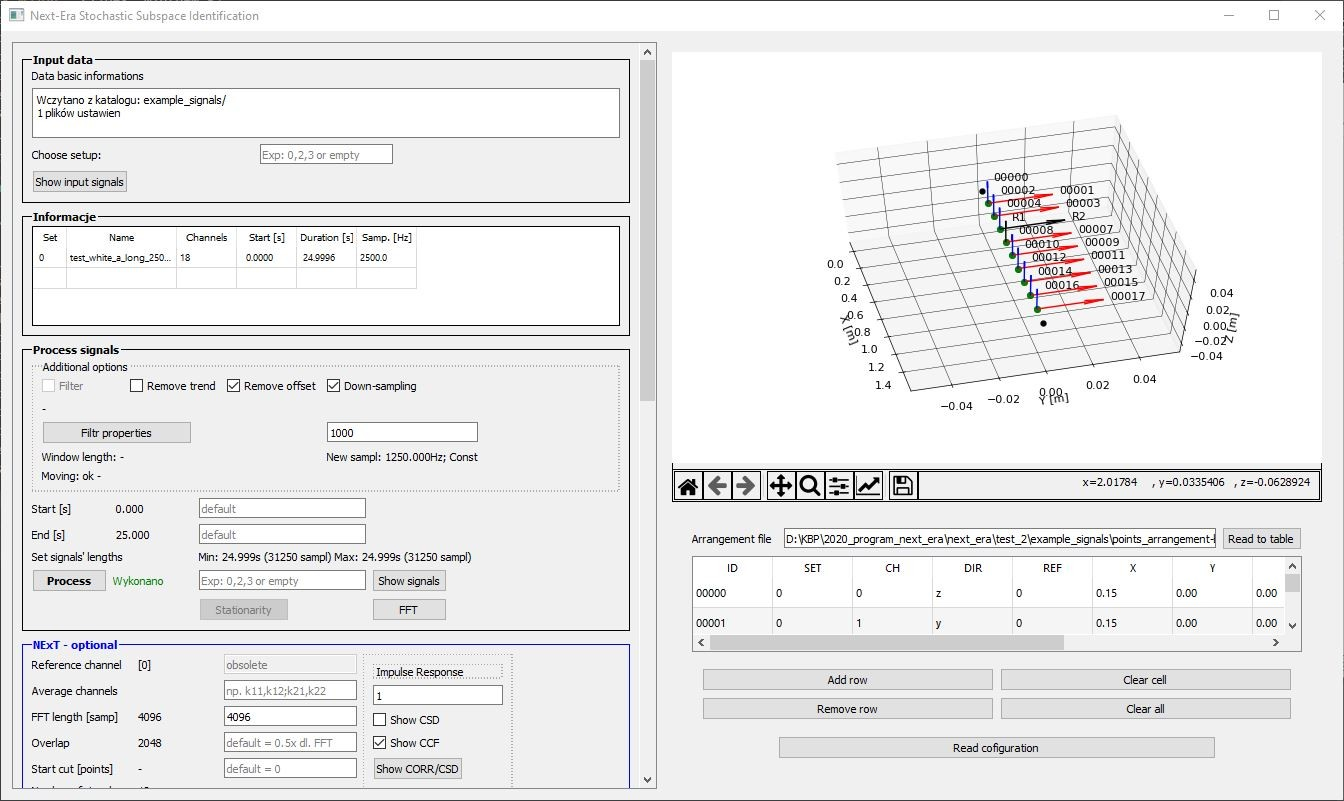
\includegraphics[width=\linewidth]{/program/okno_programu.JPG}
	\captionsetup{justification=centering}
	\caption{Widok na okno główne stworzonej aplikacji do identyfikacji modalnej}
	\label{fig: okno_programu_widok}
\end{figure}

\subsection{Algorytm programu}

Algorytm programu przedstawiono na grafice [].
Poniżej omówiono podstawowe informacje na temat użytych metod przetwarzania sygnałów.

Wstępnie sygnały wyjściowe mogą być poddane standardowemu przetwarzaniu sygnału. Do zastosowanych metod należy filtrowanie, usuwanie składowej stałej i obniżenie próbkowania \teng{downsampling, resampling}. Filtrowanie może posłużyć do odrzucenia niechcianych składowych z sygnału i ograniczyć identyfikację jedynie do określonego obszaru. Odcięcie składowej stałej jest koniecznym elementem przygotowania sygnałów do identyfikacji. Bez tego zabiegu, tak jak w przypadku Transformaty Fouriera występuje istotny pik na zerowej odciętej, tak utrudniona może być identyfikacja modów o niskiej częstotliwości. Zmiana częstotliwości próbkowania jest bardzo przydatną funkcją. Podobnie do filtrowania zmniejsza zakres analizowanej dziedziny, ale w odróżnieniu do filtrowania zmniejsza również liczbę próbek sygnału. Należy pamiętać, że resampling nie jest tożsamy pominięciu części próbek z sygnału. Wpływ obróbki sygnału na wyniki identyfikacji oraz zalecenia dotyczące przyjmowanych parametrów opisał \cite{Caicedo2011} 


Pierwszym głównym etapem w algorytmie NExT-ERA jest wyznaczenie funkcji korelacji wprowadzonych sygnałów. Wyznaczanie funkcji korelacji metodą bezpośrednią jest wymagające obliczeniowo. Z tego powodu wykorzystuje się zależność pomiędzy gęstością widmową mocy, a funkcją korelacji (\ref{eq: spectralDensity} i \ref{eq: correlationInversSpectralDensity}). Wyznaczenie gęstości widmowej mocy jest możliwe za pomocą znacznie bardziej efektywnych algorytmów. Jednym z nich jest metoda Welch'a \parencite{Welch1967,Brincker2015}, którą zastosowano w programie. Umożliwiono również łączenie i uśrednianie wielu serii pomiarowych w jeden wynik identyfikacji. Wykorzystano do tego algorytm przedstawiony w \cite{Brownjohn2010}. W przypadku łączenia serii pomiarowych w jeden wynik, konieczne jest zastosowanie punktów referencyjnych. Punkty referencyjne są to punkty stałe w trakcie całych pomiarów, muszą występować w każdej serii pomiarowej i nie mogą znajdować się w węźle żadnej postaci drgań. Innymi słowy punkt referencyjny musi mieć niezerową wartość w wektorze określającym postać drgań, którą należy zidentyfikować. W zastosowanym algorytmie istnieje możliwość wyboru po jednym punkcie referencyjnym dla każdego z kierunków drgań: X, Y, Z. Łączenie serii pomiarowych odbywa się w następujący sposób:
\begin{itemize}[noitemsep]
	\item Algorytmem Welch'a wyznaczane są funkcje wzajemnych gęstości widmowych mocy pomiędzy sygnałem referencyjnym, a pozostałymi sygnałami na powiązanym kierunku.  Wzajemne gęstości widmowe związane z danym punktem referencyjnym są zestawione w jeden wektor.
	\item Wyznaczane są funkcje auto gęstości widmowych mocy dla sygnałów w punktach referencyjnych. Użyty jest do tego ten sam algorytm co w przypadku wzajemnych funkcji gęstości widmowej mocy, z tą różnicą że sygnały wejściowe są identyczne. 
	\item Funkcje wzajemnej gęstości widmowej mocy zestawione w jednym wektorze dzielone są przez funkcję auto gęstości widmowej punktu referencyjnego. W tym przypadku wymagane jest aby długość wektora wszystkich wektorów była równa. Identycznie postępuje się z każdym wektorem gęstości widmowych mocy.
	\item Auto gęstości widmowe mocy dla danego punktu referencyjnego są uśredniane. Auto gęstości widmowe mocy są sumowane ze wszystkich ustawień, a wynik jest podzielony przez liczbę ustawień.
	\item Po procesie uśredniania gęstości widmowych mocy punktów referencyjnych następuje działanie odwrotne. Wcześniej podzielone wzajemne gęstości widmowe mocy mnożone są przez uśrednione auto gęstości widmowe mocy punktów referencyjnych.
	\item Wynikowe gęstości widmowe mocy przekształcane są za pomocą odwrotnej Transformaty Fouriera do sygnałów w dziedzinie czasu. Otrzymany wynik odpowiada funkcjom cross-korelacji i może być użyty w metodzie ERA.
	
\end{itemize}

Uśrednianie serii pomiarowych z tym samym ustawieniem punktów pomiarowych odbywa się przez sumowanie gęstości widmowych mocy z powtórzonych serii pomiarowych i podzieleniu przez liczbę powtórzonych serii. Pomimo zestawienia funkcji gęstości widmowych mocy w wektory, wszystkie wspomniane wyżej operacje mnożenia i dzielenia funkcji gęstości widmowych mocy polegają na działaniu na poszczególne prążki spektrum, a nie na klasycznym rozumieniu mnożenia i dzielenia wektorów. 

\subsection{Elementy oceny poprawności rozwiązania}
Ważnym elementem w procesie identyfikacji modalnej jest ocena poprawności uzyskanego rozwiązania. W tym celu najczęściej wykorzystywane są diagramy stabilizacyjne. W przypadku pomiarów obarczonych szumem, przyjęty rząd modelu musi być zadeklarowany jako większy niż miało by to miejsce w idealnych warunkach. Diagram stabilizacyjny pozwala na określenie minimalnego rzędu modelu, przy którym występują wszystkie interesujące mody i są one stabilne. Zastosowanie diagramów stabilizacyjnych opisano między innymi w (!!!). W programie zastosowano dwie wersje diagramów: niefiltrowaną i filtrowaną. Wersja niefiltrowana obrazuje wszystkie wyznaczone mody: rzeczywiste i fikcyjne. Odróżnia je w zależności od wyników dla niższego rzędu modelu. Jeśli istnieje w modelu o rząd niższym mod spełniający odpowiednie kryteria to jest on uznany za rzeczywisty. Dla rzędu modelu $n$ i obliczonego modu $i$ zastosowane w programie domyślne kryteria to:
\begin{itemize}[noitemsep]
	\item częstotliwość $f$ w dwóch kolejnych krokach nie może się różnić o więcej niż 1\%,
	\begin{equation}\label{eq: stabdiag_crit_freq}
		\Delta f =  \Big| 1-\frac{f_{n,i}}{f_{n+1,i}}\Big|  \le 0.01
	\end{equation}
	\item tłumienie $\xi$ w dwóch kolejnych krokach nie może się różnić o więcej niż 5\%,
		\begin{equation}\label{eq: stabdiag_crit_ksi}
		\Delta \xi =  \Big| 1-\frac{\xi_{n,i}}{\xi_{n+1,i}}\Big|  \le 0.05
	\end{equation}
	\item parametr MAC dla postaci w dwóch kolejnych krokach musi być większy niż 0.95,	
	\item parametr MPC postaci modu musi być większy niż 0.9.
	\begin{equation}\label{eq: stabdiag_crit_MPC_MAC}
		\text{MAC}_i^{n,n+1} \ge 0.95 \qquad \text{MPC}_i \ge 0.90
	\end{equation}
\end{itemize}
Diagram niefiltrowany obrazuje rozkład zidentyfikowanych modów w domenie częstotliwości. Wstępnie pozwala ocenić czy istnieją mody stabilne (częstotliwość i tłumienie), o rzeczywistych wektorach postaci (MPC) i o niezmiennej formie (MAC). W przypadku dużego rzędu modelu i bliskich sobie modów trudno jednoznacznie odnaleźć jedynie poprawne rozwiązania. Z tego względu stworzono również wersję filtrowaną diagramu stabilizacyjnego. Diagram filtrowany w znacznie bardziej czytelny sposób pozwala przedstawić jedynie mody uznane za rzeczywiste. Jego generacja opiera się na następujących krokach:
\begin{itemize}[noitemsep]
	\item Podział dziedziny częstotliwości na wąskie pasma (np. 1\% dolnej granicy pasma) i podział wszystkich punktów według przynależności do poszczególnych pasm,
	\item Odrzucenie punktów, dla których tłumienie jest zbyt duże ($\text{LDT}\ge0.3$) lub ujemne,
	\item Wyznaczenie parametru MAC pomiędzy wszystkimi punktami w paśmie oraz parametru MPC dla każdego modu w paśmie.
	\item Wyznaczenie wartości średniej i odchylenia standardowego częstotliwości, tłumienia i parametrów MAC i MPC dla punktów pasma. Jeżeli wartości średnie pomniejszone o odchylenie standardowe są spełniają dopuszczalne warunki, to zestaw punktów uznany jest za określający rzeczywisty mod. Jeżeli nie, wyszukiwany jest punkt charakteryzujący się najgorszym parametrem MAC lub MPC albo zbyt różniącą się liczbą tłumienia i jest odrzucany. Następnie ponownie oceniana jest wartość średnia i odchylenie standardowe. Proces ten toczy się do momentu odrzucenia wszystkich punktów lub spełnienia kryteriów uznania mod za rzeczywisty.
	\item Ostatecznie jako rzeczywiste i stabilne określane są mody, dla których liczba punktów w paśmie jest większa od wartości minimalnej. Domyślnie jest to 20\% maksymalnego rzędu modelu na diagramie.
\end{itemize}
Wskaźniki MAC i MPC są istotną częścią algorytmu programu i służą ocenie poprawności wyników. Poniżej przytoczono ich definicje i podstawowe właściwości. 

\subsubsection{Model Phase Colinearity (MPC)}
Wynikiem przeprowadzonej analizy modalnej są postaci i częstotliwości o wartościach zespolonych. Postaci zidentyfikowane na podstawie pomiarów wartości rzeczywistych powinny stanowić wektory o współrzędnych rzeczywistych. W przypadku modów normalnych wszystkie punkty konstrukcji drgają dokładnie w fazie lub w przeciw fazie względem siebie. Przeciwnie, kiedy postaci są wektorami zespolonymi, przemieszczenia osiągają wartości ekstremalne w różnych chwilach czasowych dla różnych stopni swobody. \cite{Ewins2000,Chopra2012a} podają przykładowe przyczyny powstania postaci o wektorach zespolonych. Są to m.in. efekt żyroskopowy, efekty aerodynamiczne, nieliniowość czy nieproporcjonalne tłumienie. Zidentyfikowane mody zwykle występują w postaci zespolonej. Wynika to z relatywnie niskiego wskaźnika sygnału do szumu \parencite{Rainieri2014}. Mimo to, "stopień zespolenia" jest zwykle niewielki i w praktycznych zastosowaniach błąd wynikający z tej cechy może być zaniedbany. Mimo to ważnym jest żeby rozróżnić, które mody są normalne, a które w dużej mierze zespolone. Jedną z najprostszych metod jest wykreślenie współrzędnych składników postaci w układzie biegunowym. Metoda została szerzej opisana w \parencite{Ewins2000}. Zasadą jest, że jeśli w konstrukcji występuje tłumienie proporcjonalne to składniki danej postaci układają się na linii prostej w zespolonym układzie współrzędnych \parencite{Rainieri2014}).
Do ilościowego określenia stopnia przestrzennej spójności modu \cite{Pappa1992} opracowali wskaźnik MPC (\textit{Modal Phase Collinearity}). Jest on dla $i$-tego moda określony wzorem \ref{eq:mpc_ratio}
\begin{equation}
	{S}_{xx}={\mathbf{\Phi}'}_{i}^{\mathsf{T}} {\mathbf{\Phi}} '_{i} \quad
	%\end{equation}
	%\begin{equation}
	{S}_{yy}={\mathbf{\Phi}''}_{i}^{\mathsf{T}} {\mathbf{\Phi}}''_{i} \quad
	%\end{equation}
	%\begin{equation}
	{S}_{xy}={\mathbf{\Phi}'}_{i}^{\mathsf{T}} {\mathbf{\Phi}}''_{i}
\end{equation}
\begin{equation}
	{\mu}=\frac{S_{xx}-S_{yy}}{2S_{xy}} \quad \quad
	\beta=\mu+\mathrm{sgn}(S_{xy})\sqrt{\mu^{2}+1} \quad \quad
	\tau=\tan^{-1}{(\beta)} \quad
\end{equation}
\begin{equation}
	\lambda_{1}=S_{xx}+\frac{S_{xy}(2(\mu^{2}+1)\sin^{2}{(\tau)}-1)}{\mu}
\end{equation}
\begin{equation}
	\lambda_{2}=S_{yy}+\frac{S_{xy}(2(\mu^{2}+1)\sin^{2}{(\tau)}-1)}{\mu}
\end{equation}
\begin{equation} \label{eq:mpc_ratio}
	\mathrm{MPC}_{i}=\left[2\cdot\left(\frac{\lambda_{1}}{\lambda_{1}+\lambda_{2}}-0.5\right)\right]^{2}
\end{equation}
gdzie $\mathrm{sgn}(\cdot)$ oznacza funkcję zwracającą znak liczby. Wskaźnik MPC jest bezwymiarowy i przyjmuje wartości z zakresu od 0 (dla modów z zupełnie nieskorelowanymi kątami fazowymi) do 1 (dla modów jednofazowych).
\subsubsection{Modal Assurance Criterion (MAC)}

Kryterium MAC (Modal Assurance Criterion) pozwala ocenić miarę dopasowania (stopień liniowości) dwóch wektorów modalnych \parencite{Allemang1982}. Jest to podstawowe i najbardziej popularne kryterium służące porównaniu wektorów modalnych \cite{Rainieri2014}. Jego wartość waha się od 0 (dla braku dopasowania) do 1 (dla idealnego dopasowania). Definicja wskaźnika dana jest wzorem \ref{eq: MAC_definition}.
\begin{equation} \label{eq: MAC_definition}
	\text{MAC}_n = \frac{ (\vect{\psi_{n,a}}^H\vect{\psi_{n,e}})^2}
	{\vect{\psi_{n,a}}^H\vect{\psi_{n,a}}\vect{\psi_{n,e}}^H\vect{\psi_{n,e}}}
\end{equation}
gdzie $\vect{\psi_{n,a}}$ i $\vect{\psi_{n,e}}$ to wektory postaci drgań własnych, a $(\cdot)^H$ oznacza sprzężenie Hermitowskie wektora.
Należy pamiętać, że kryterium MAC nie wskazuje czy rozwiązanie jest poprawne lub czy wektory modalne są ortogonalne. Wynik pokazuje jedynie dopasowanie dwóch wektorów. Wskaźnik MAC jest nieodporny na błędy zawarte jednocześnie w obu wektorach. Z tego względu za każdym razem należy kontrolować założenia metody. Zbiór wskazówek do stosowania kryterium MAC w swojej pracy zawarł \cite{Allemang2003}. Poza swoistą instrukcją użycia wskaźnika, wskazuje on następujące główne przyczyny niemiarodajnych wyników przy korzystaniu z kryterium MAC:
\begin{itemize}[noitemsep]
	\item traktowanie kryterium MAC jako informacji o ortogonalności wektorów,
	\item nieprawidłowe matematyczne sformułowanie kryterium, głównie zastąpienie sprzężenia Hermitowskiego transpozycją. Zmiana ta jest słuszna wyłącznie przy rzeczywistych wektorach modalnych,
	\item duże różnice w wartościach współrzędnych wektorów. Kryterium jest bardzo wrażliwe na duże wartości, a niewrażliwe na małe wartości,
	\item przyjęcie zbyt małej liczby współrzędnych wektora,
	\item wypełnienie zerami współrzędnych wektora, na temat których nie ma żadnej informacji.
\end{itemize}

Ze względu na ograniczenia kryterium MAC, od momentu jego powstania powstał szereg pokrewnych wskaźników. Są to między innymi: Coordinate Modal Assurance Criterion (COMAC) \parencite{Ewins2000}, Enhanced Coordinate Modal Assurance Criterion (ECOMAC) \parencite{Hunt1992} czy Inverse Modal Assurance Criterion (IMAC) \parencite{MITCHELL1998}. Każde z kryteriów zostało zmodyfikowane w celu wyeliminowania konkretnego ograniczenia oryginalnej wersji. Zestawienie i opis wielu z nich przedstawiono miedzy innymi w pracach \parencite{Allemang2003,Rainieri2014,Szafranski2013,Salamak2003} 

Poza diagramem stabilizacyjnym, w niniejszej pracy kryterium MAC zostało również użyte przy doborze lokalizacji czujników w trakcie pomiarów na konstrukcji rzeczywistej. Jest to kolejne z popularnych zastosowań współczynnika MAC \parencite{Allemang2003}. Polega na takim doborze punktów pomiarowych, aby zidentyfikowane w tych punktach postaci drgań były od siebie maksymalnie różne. Opis przyjętego rozwiązania i wyniki obliczeń przedstawiono w wynikach badań w rozdziale \ref{sect: identyfikacja_modalna_wk2}.




\subsection{Testy numeryczne metody NEXT-ERA}
Każda aplikacja komputerowa przed użyciem powinna być poddana testom. W przypadku aplikacji służącej celom naukowym, gdzie zakłada się pewien poziom wiedzy i świadomości użytkownika zdecydowano, że testom poddane zostanie jedynie jądro programu - algorytm NExT-ERA. W tym celu założono wykonanie dwóch testów: numerycznego i laboratoryjnego. Test numeryczny ma opierać się na wykonaniu modelu obliczeniowego w oprogramowaniu MES, a następnie obciążeniu go losowo (w przybliżeniu szumem białym) i wykonaniu analizy dynamicznej. Test laboratoryjny ma polegać na pomiarze i analizie drgań środowiskowych rzeczywistego obiektu badawczego. Celem testu nie jest uzyskanie idealnej zgodności pomiędzy wynikami z badania numerycznego i laboratoryjnego, a jedynie sprawdzenie działania programu. Wyniki uzyskane z testu numerycznego są pozbawione wpływu wielu niedokładności, takich jak szumów, nieliniowych warunków brzegowych, nieosiowo ustawionych czujników czy wzajemnego wpływu składowych ortogonalnych na mierzone wartości. Dlatego traktowane są głównie jako test algorytmu. Mogą również służyć jako punkt odniesienia do wyników badań laboratoryjnych. Z kolei badania laboratoryjne pozwolą sprawdzić czy program i system pomiarowy są odporne na rzeczywiście występujące obciążenia procesu identyfikacji.

Przedmiotem badań była konstrukcja o schemacie statycznym bliskim belce swobodnie podpartej. Głównym elementem układu jest kształtownik stalowy o przekroju ceowym C40 i o długości 1.5m. Obiekt został opisany szerzej w punkcie \ref{sect: next_era_lab_test}).  Model numeryczny wykonano w programie MES bazujac na inwentaryzacji wymiarów obiektu laboratoryjnego. Założono, że głównym aspektem porównawczym z badaniami laboratoryjnymi mają być mody giętne pionowe. Z tego powodu znacznie uproszczono względem rzeczywistości strefy podporowe. Nie wykonano żadnej kalibracji modelu, aby odpowiadał lepiej strukturze rzeczywistej. Do budowy wykorzystano środowisku MES SOFiSTiK. Dla odwzorowania całego układu użyto jednowymiarowych elementów belkowych. Wizualizację oraz schemat statyczny pokazano na rysunku \ref{fig: test_beam_wis_model}.
\begin{figure}[h]
	\centering
	\subfloat[Wizualizacja]{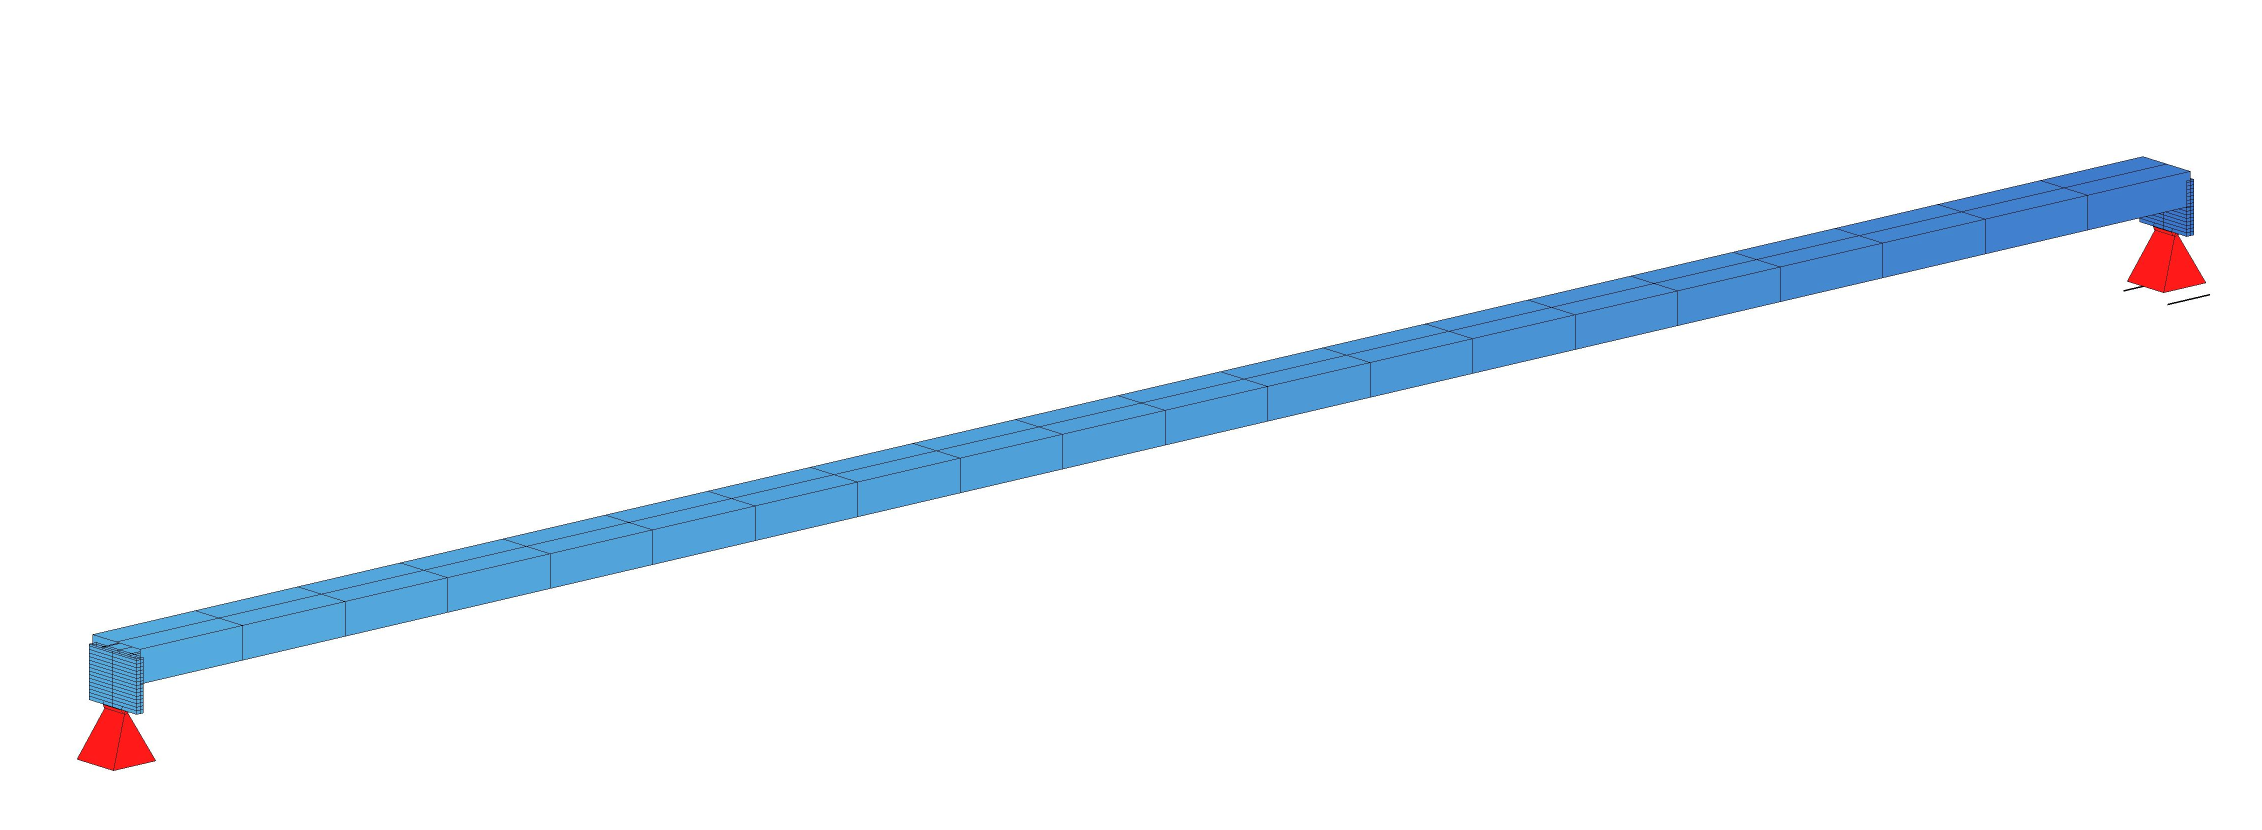
\includegraphics[width=0.5\linewidth]{/test_blue/sof_wis/wis_small002.png}}%
	\subfloat[Schemat statyczny]{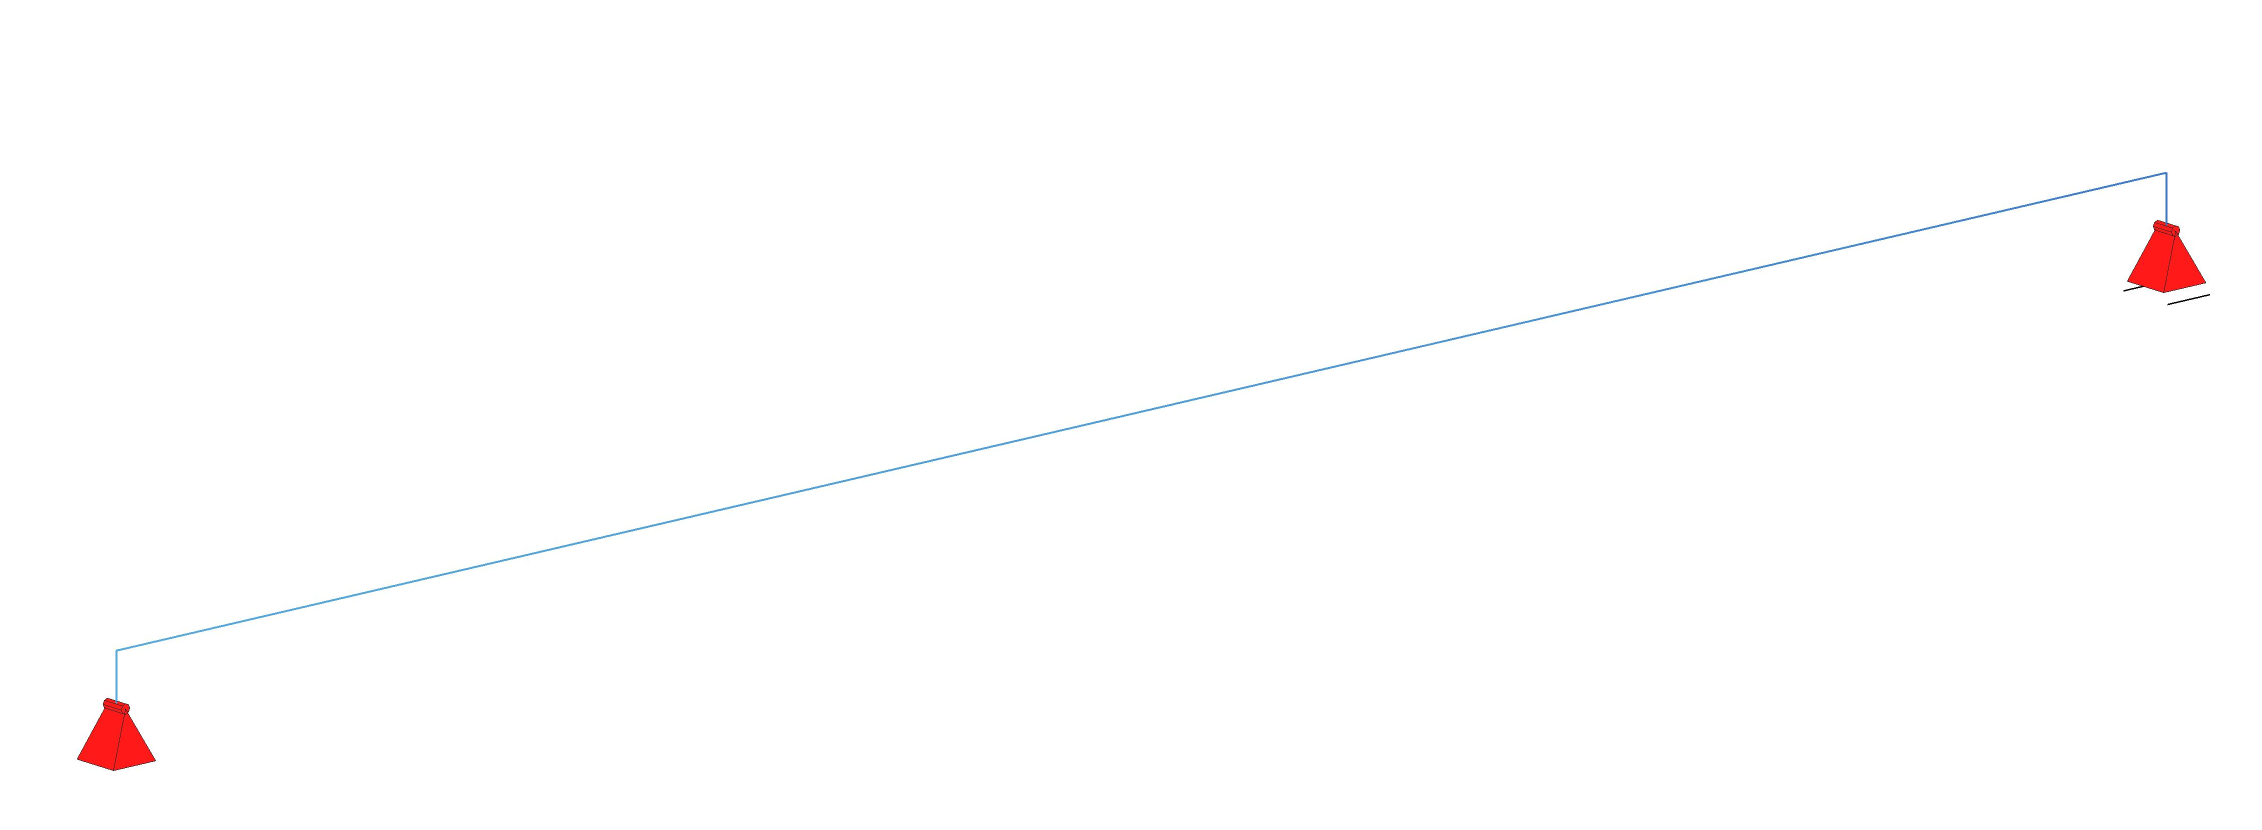
\includegraphics[width=0.5\linewidth]{/test_blue/sof_wis/wis_small001.png}}%
	\captionsetup{justification=centering}
	\caption{Wizualizacja i schemat statyczny testowego modelu numerycznego}
	\label{fig: test_beam_wis_model}
\end{figure}




Przed przystąpieniem do analizy wygenerowano 5000 losowych przypadków obciążenia. Losowy charakter uzyskano za pomocą następujących założeń dla każdego przypadku obciążenia:
\begin{itemize}[noitemsep]
	\item w każdym węźle pośrednim może, ale nie musi, być przyłożona siła pionowa lub poprzeczna,
	\item jeśli siła została przyłożona, jej wartość jest losowana z zakresu od -3 do 3 N dla każdego węzła indywidualnie,
	\item w trakcie analizy, w każdym kroku czasowym losowany jest jeden przypadek obciążenia z wygenerowanych 5000.
\end{itemize}
Rozwiązano problem własny dynamiki przedmiotowego modelu i otrzymano rezultaty jak na rysunku \ref{fig: modal_mods_blue_beam}.

\begin{figure}[h]
	\centering
	\subfloat[Mod 1, $f_1=19.70 \text{Hz}$]{\label{fig: test_blue_sof_mod1}%
		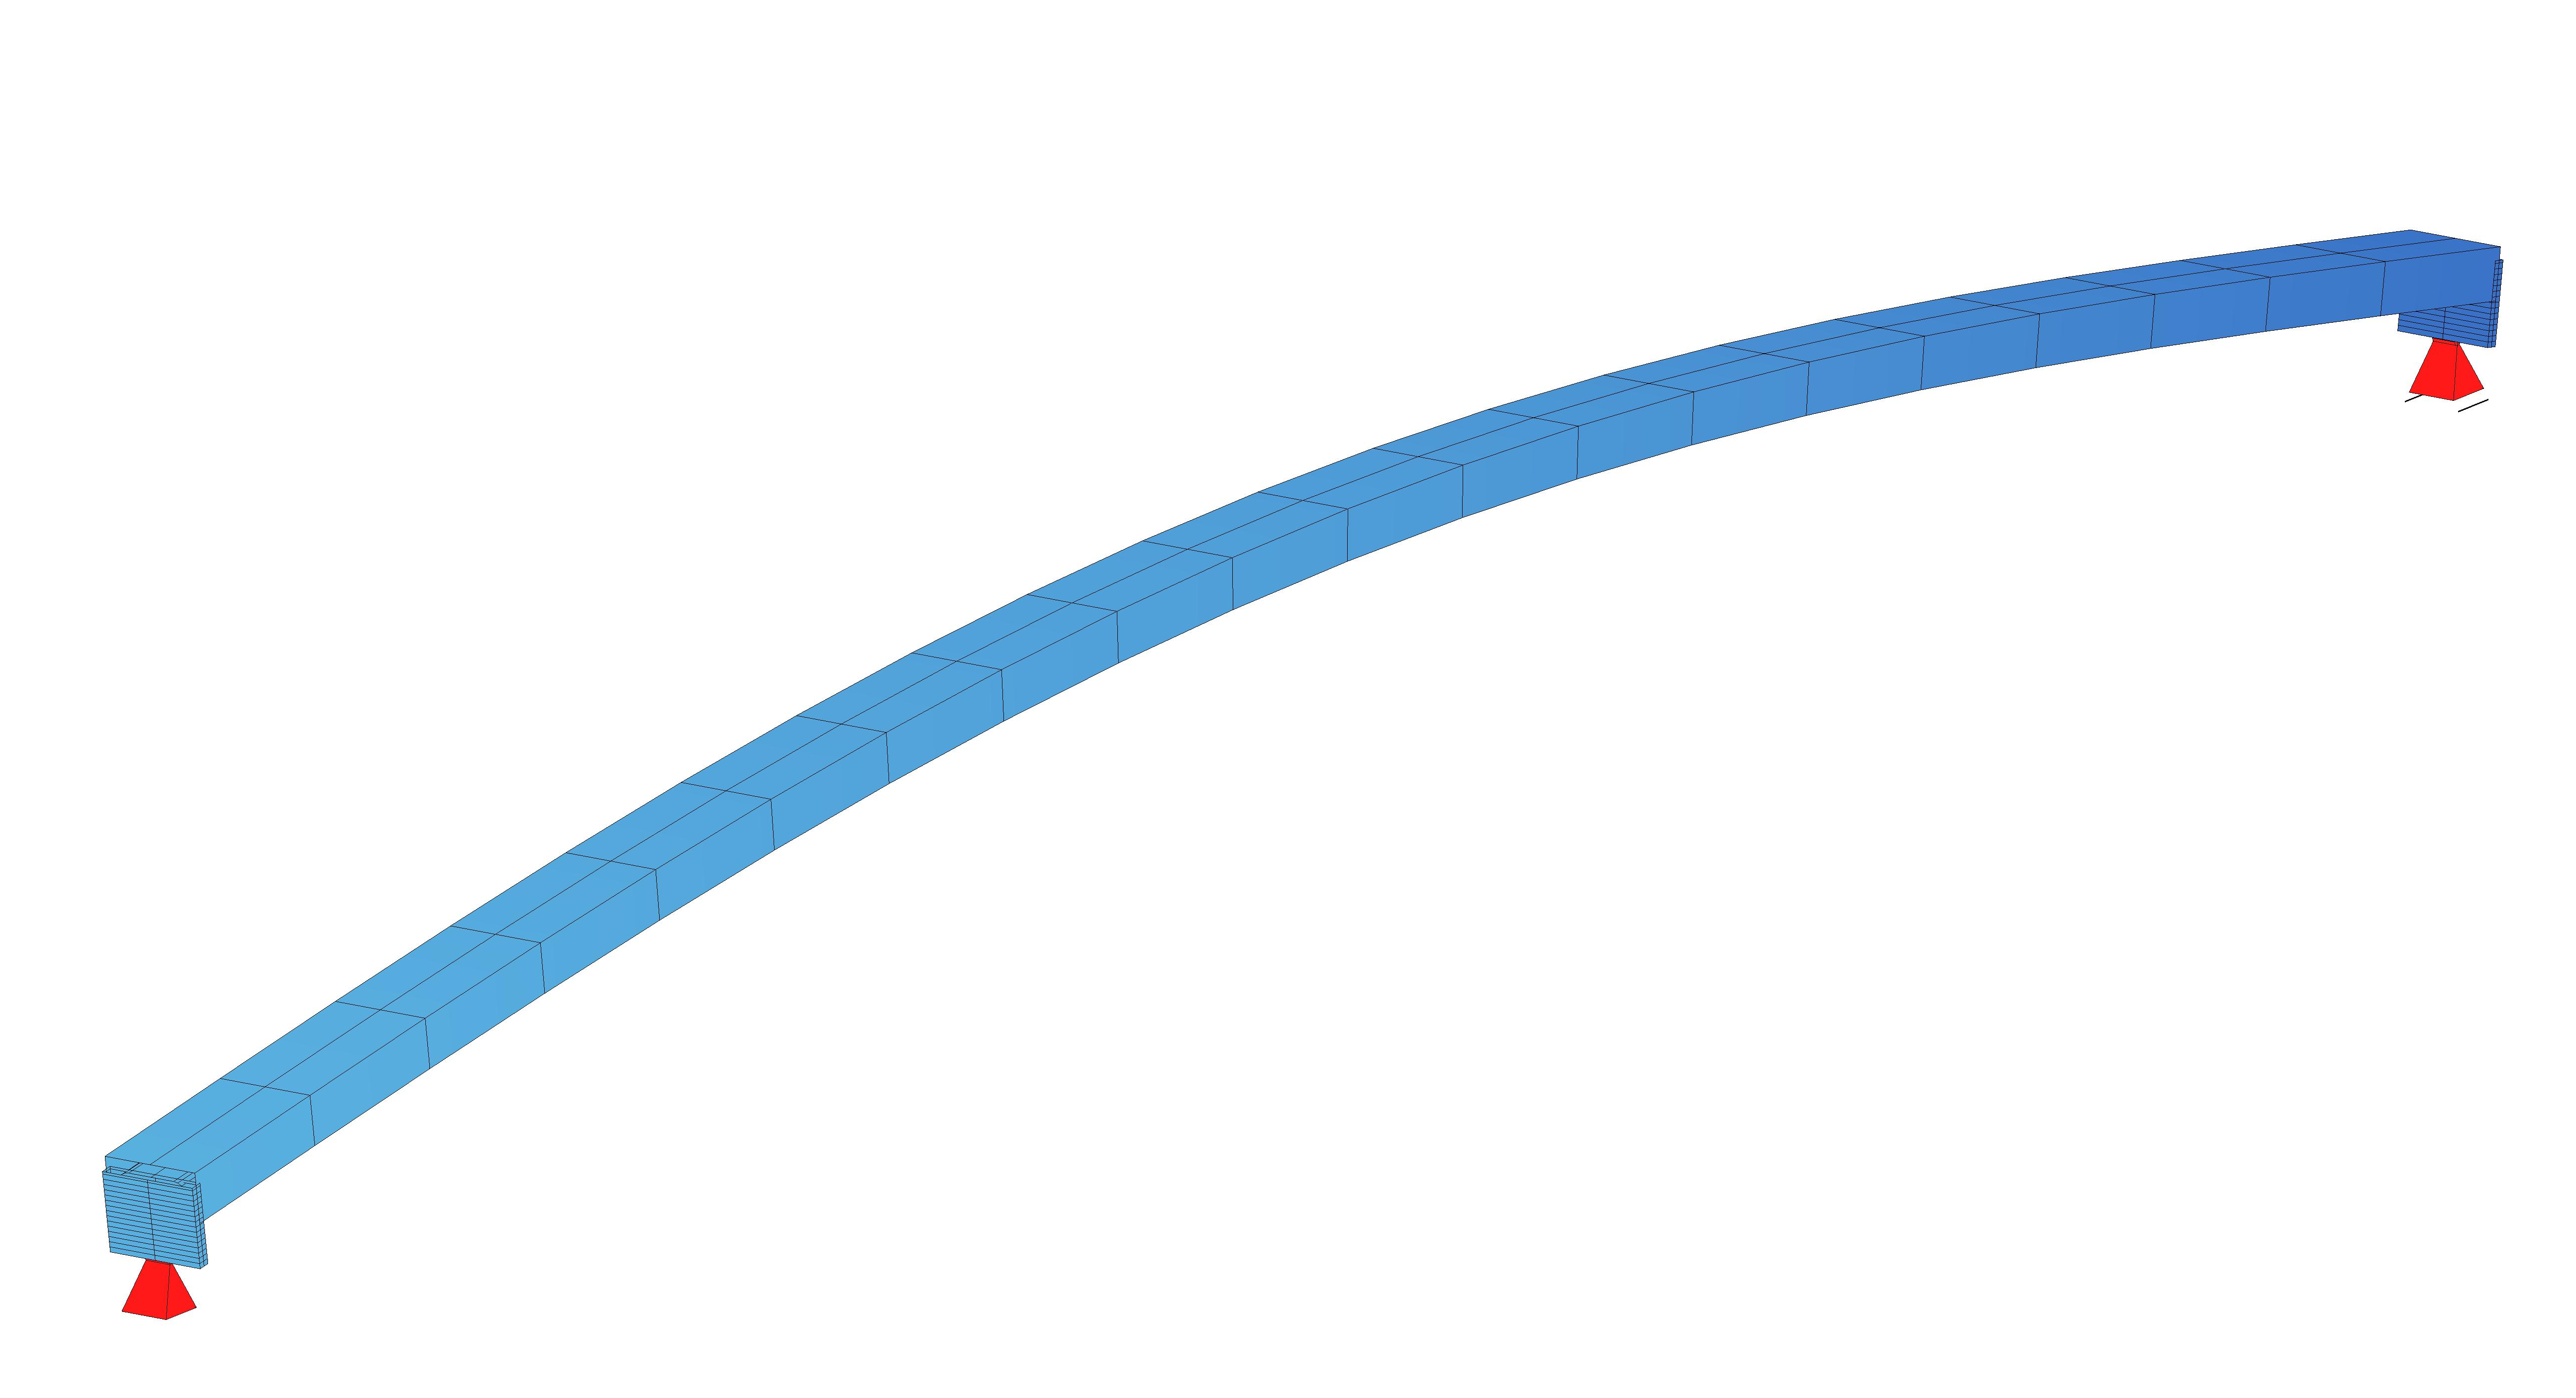
\includegraphics[width=0.33\linewidth]{/test_blue/sof_wis/image_small001.png}}%
	\subfloat[Mod 2, $f_2=54.93 \text{Hz}$]{\label{fig: test_blue_sof_mod2}%
		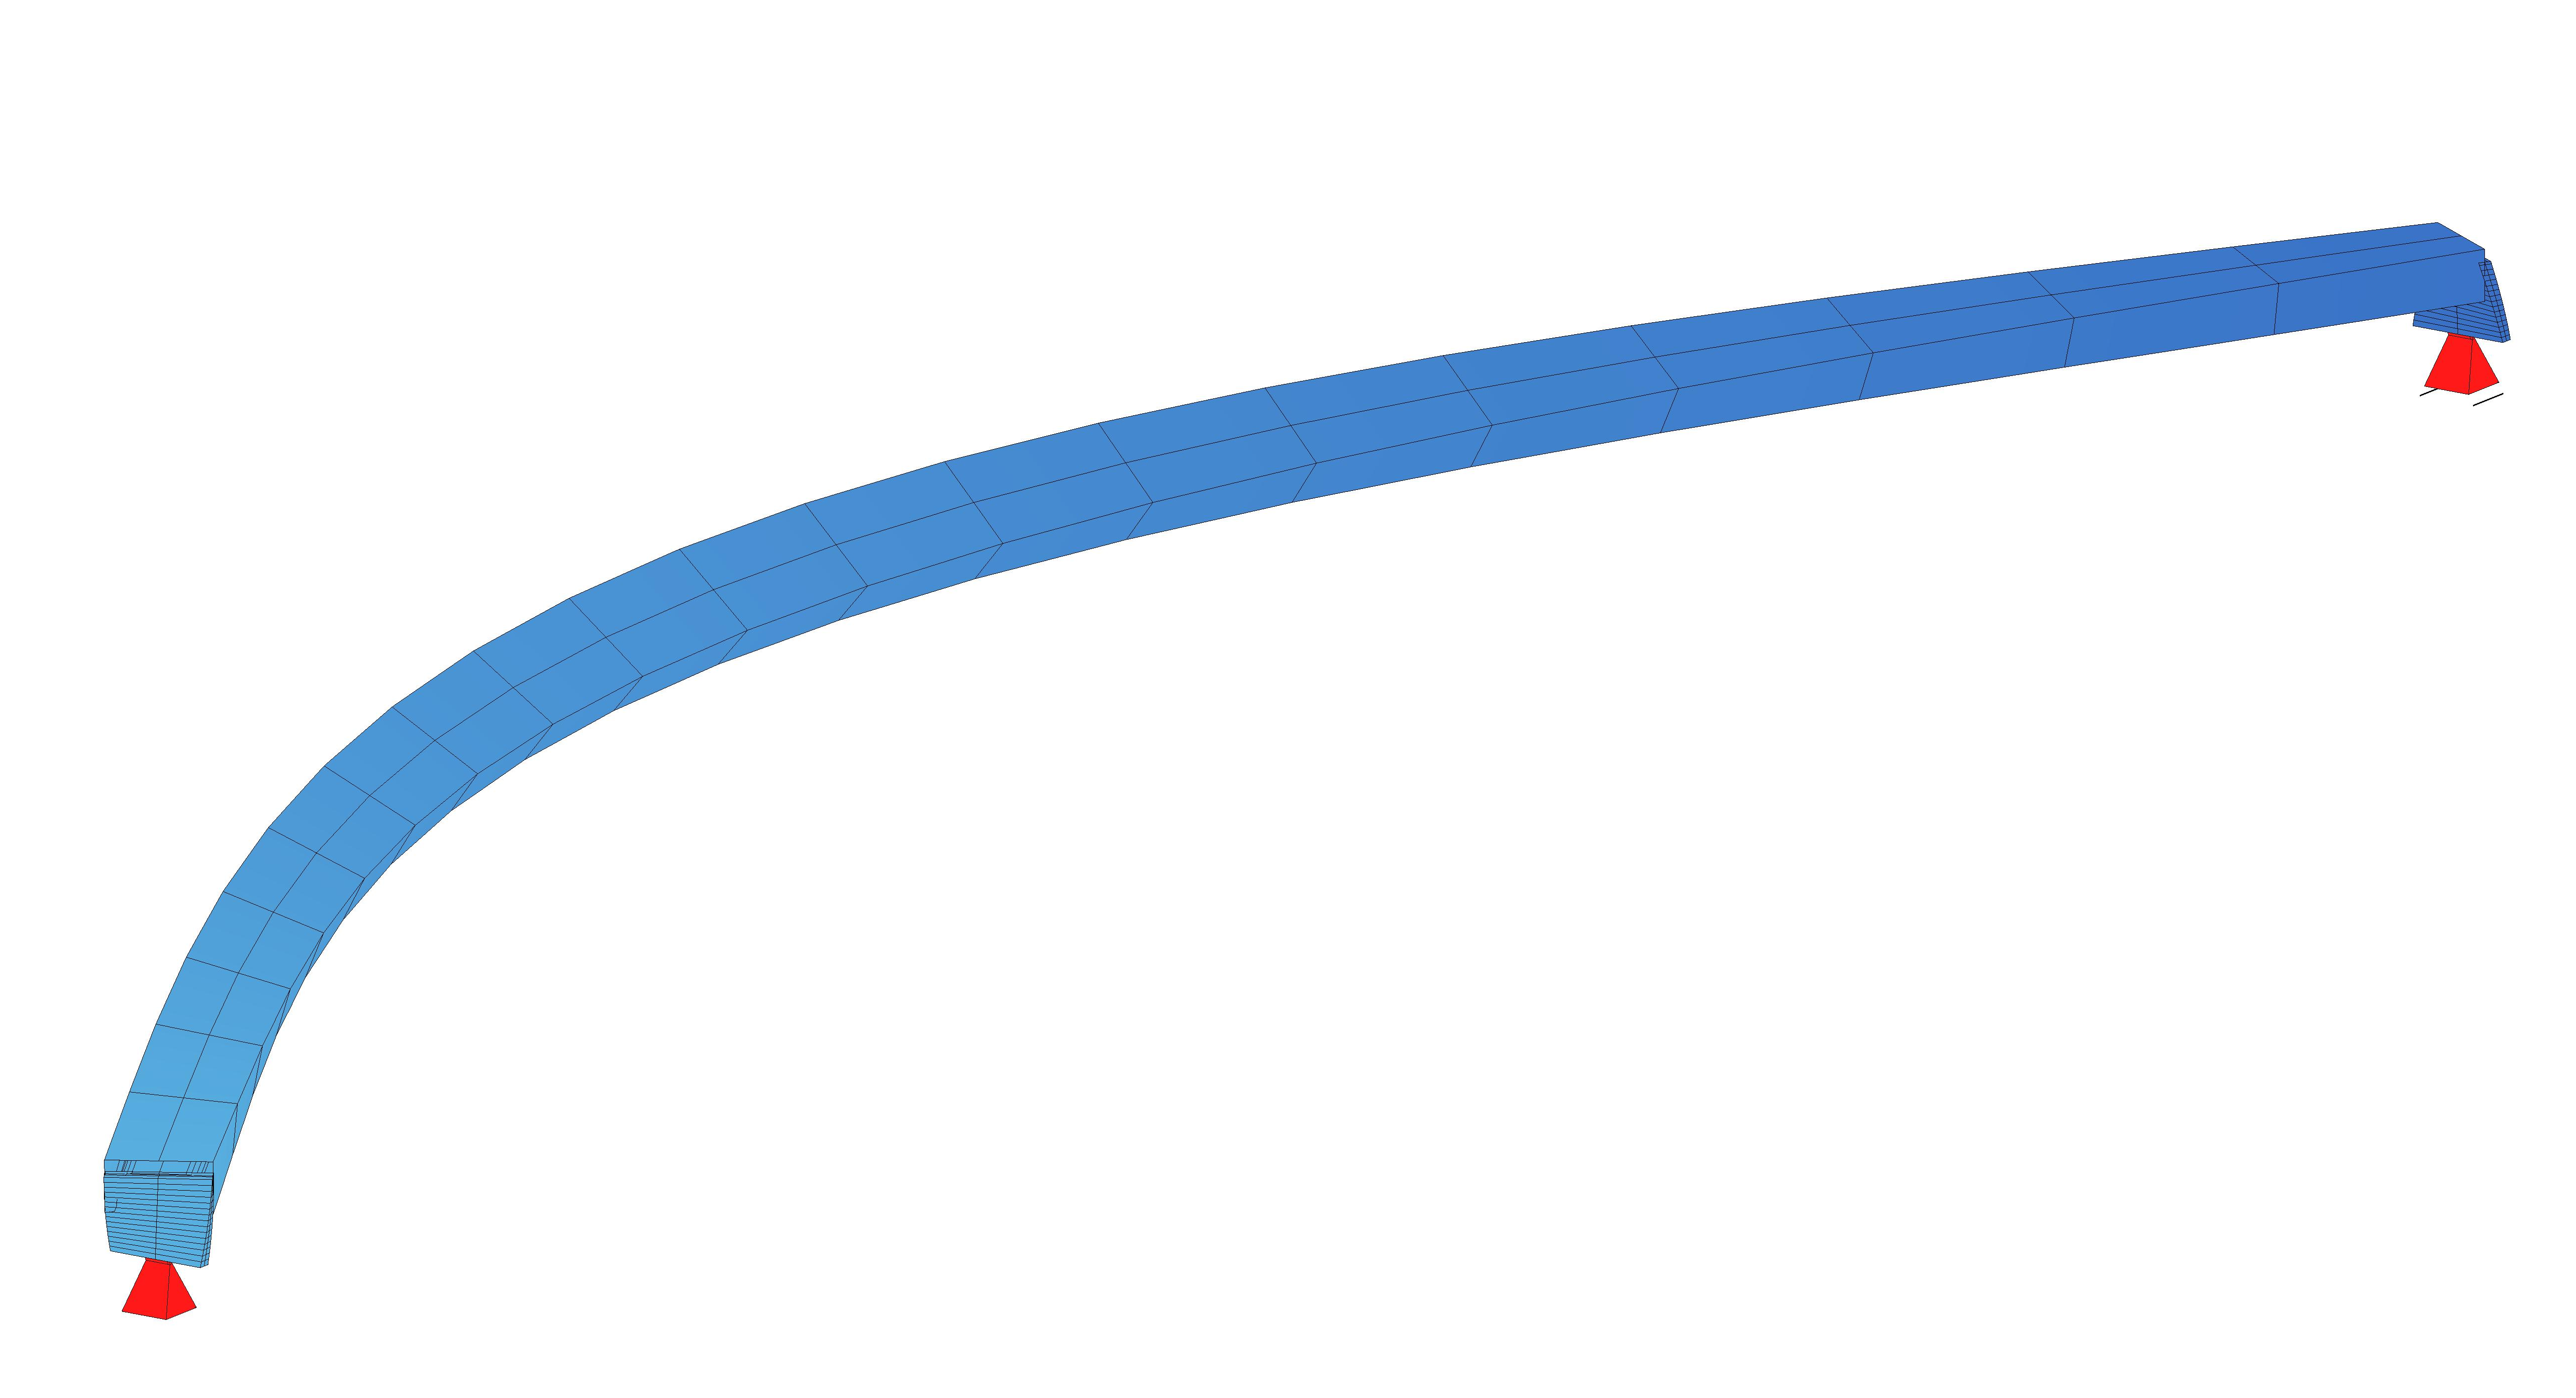
\includegraphics[width=0.33\linewidth]{/test_blue/sof_wis/image_small003.png}}%	
	\subfloat[Mod 3, $f_3=78.20 \text{Hz}$]{\label{fig: test_blue_sof_mod3}%
		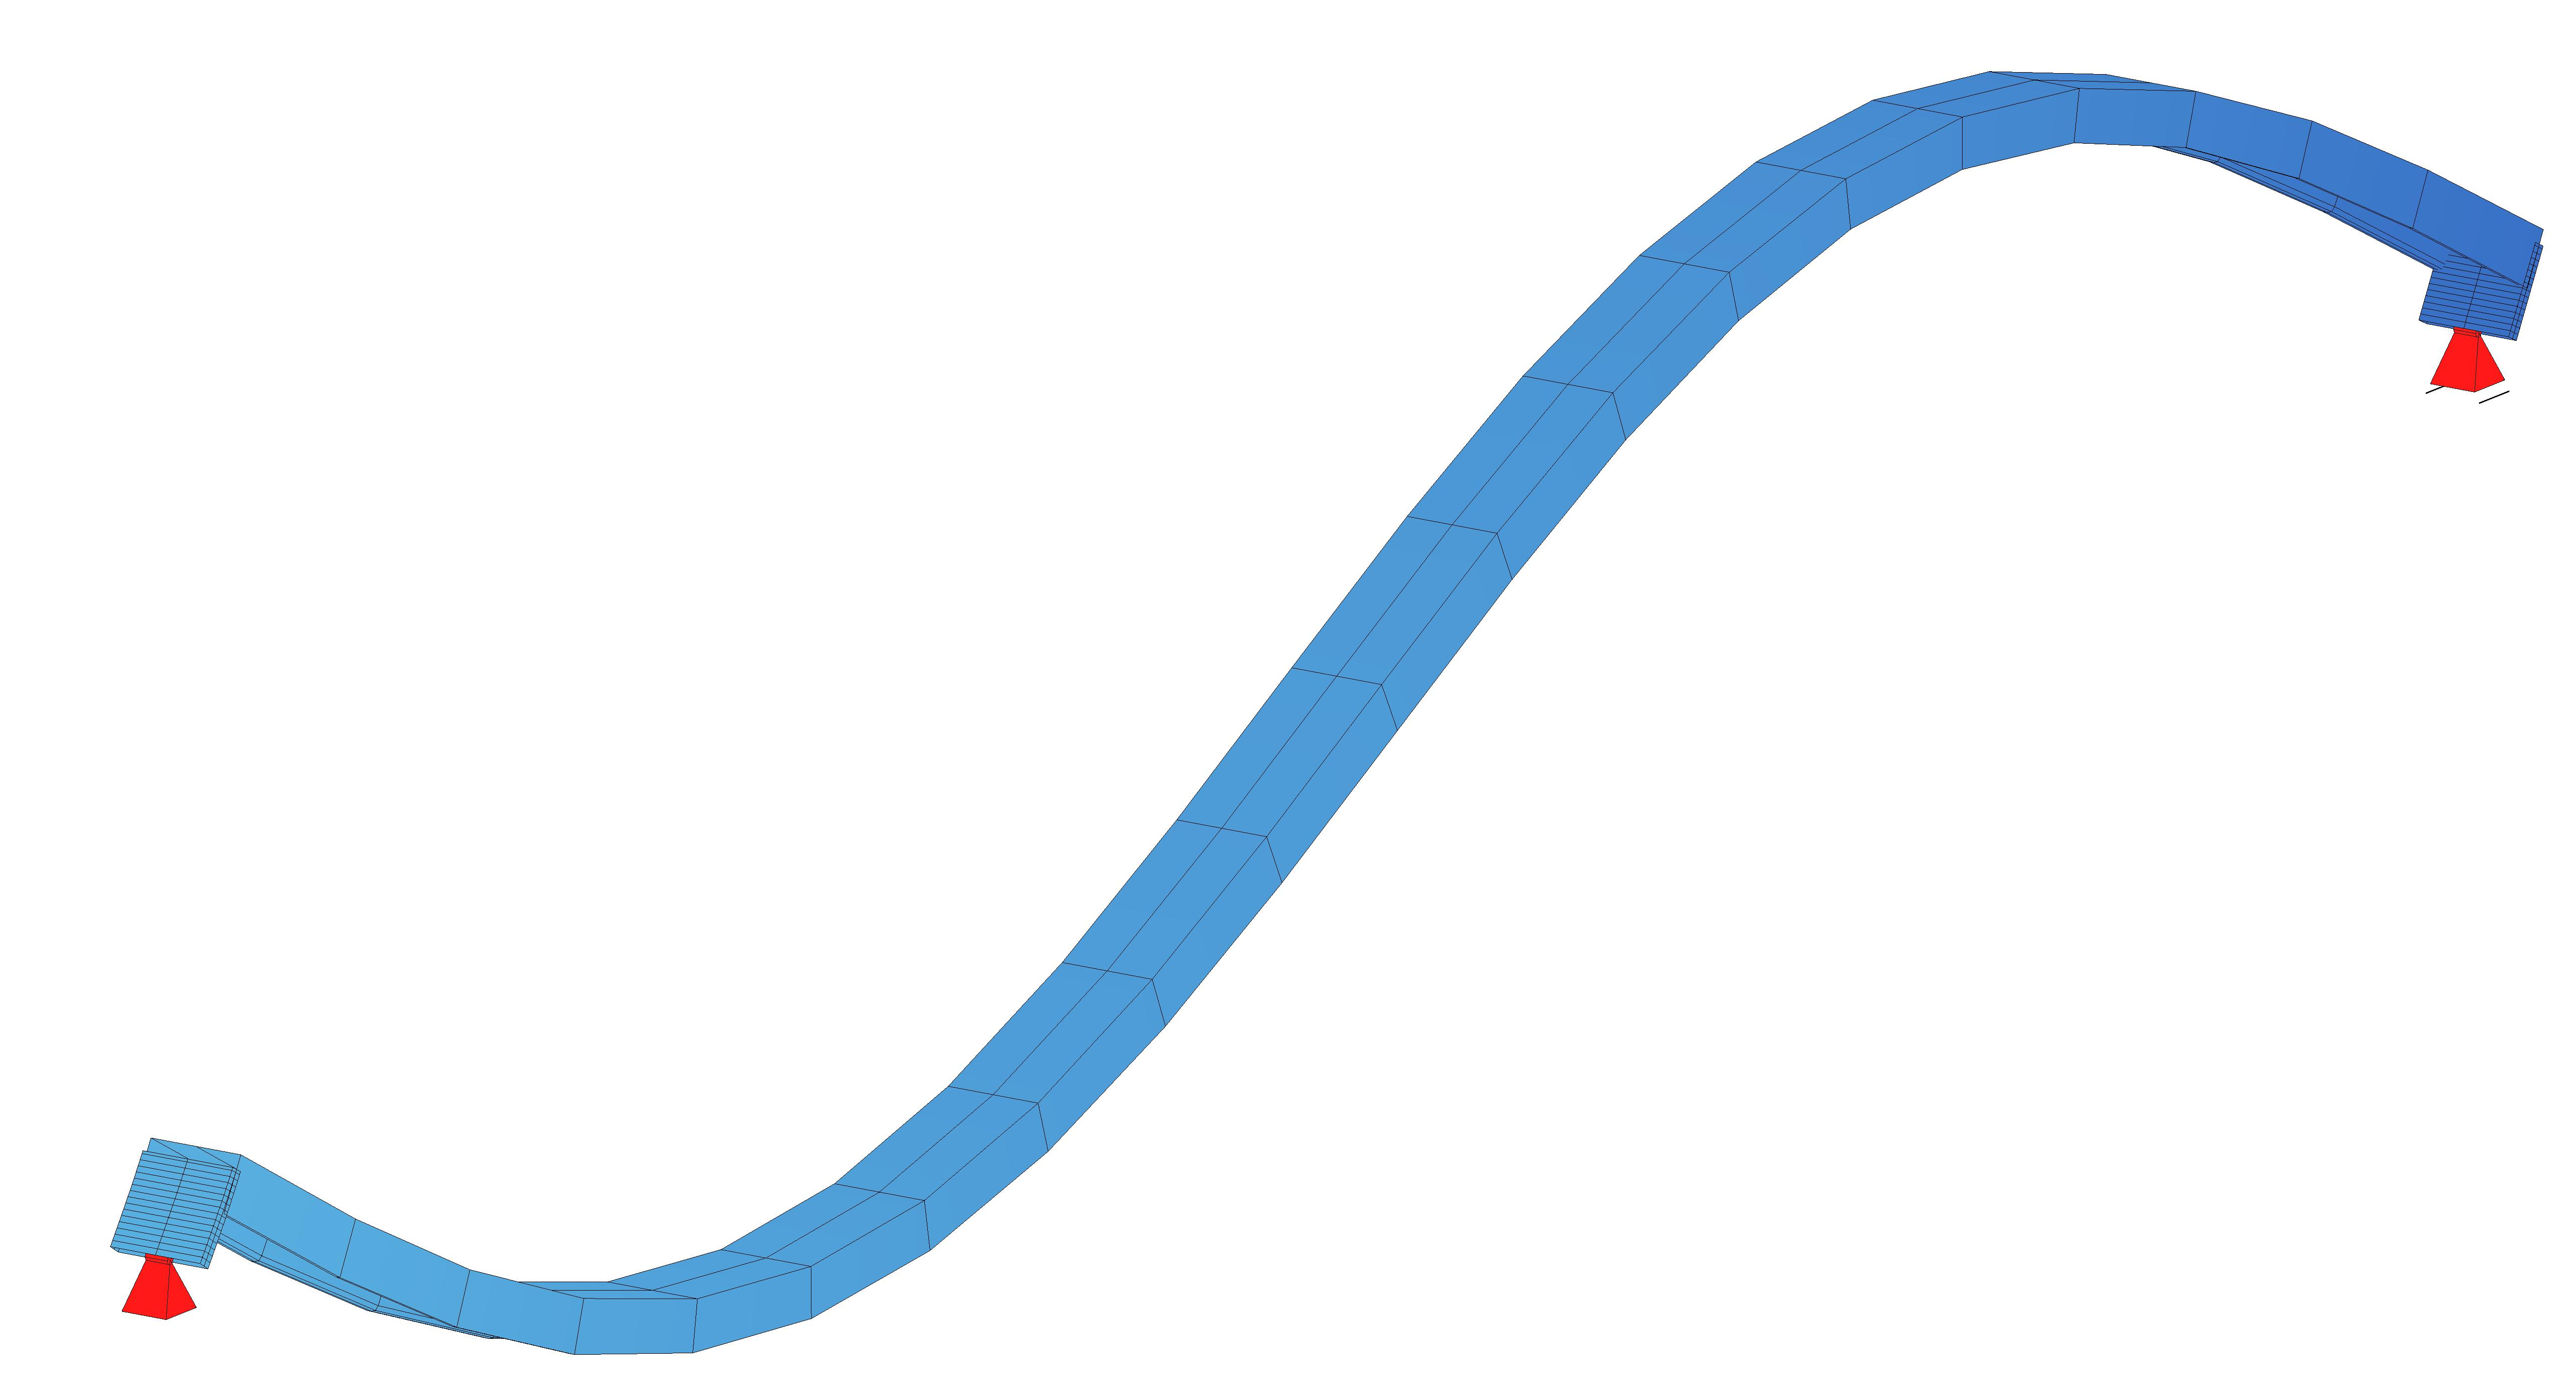
\includegraphics[width=0.33\linewidth]{/test_blue/sof_wis/image_small004.png}}\\		
	\subfloat[Mod 4, $f_4=161.35 \text{Hz}$]{\label{fig: test_blue_sof_mod4}%
		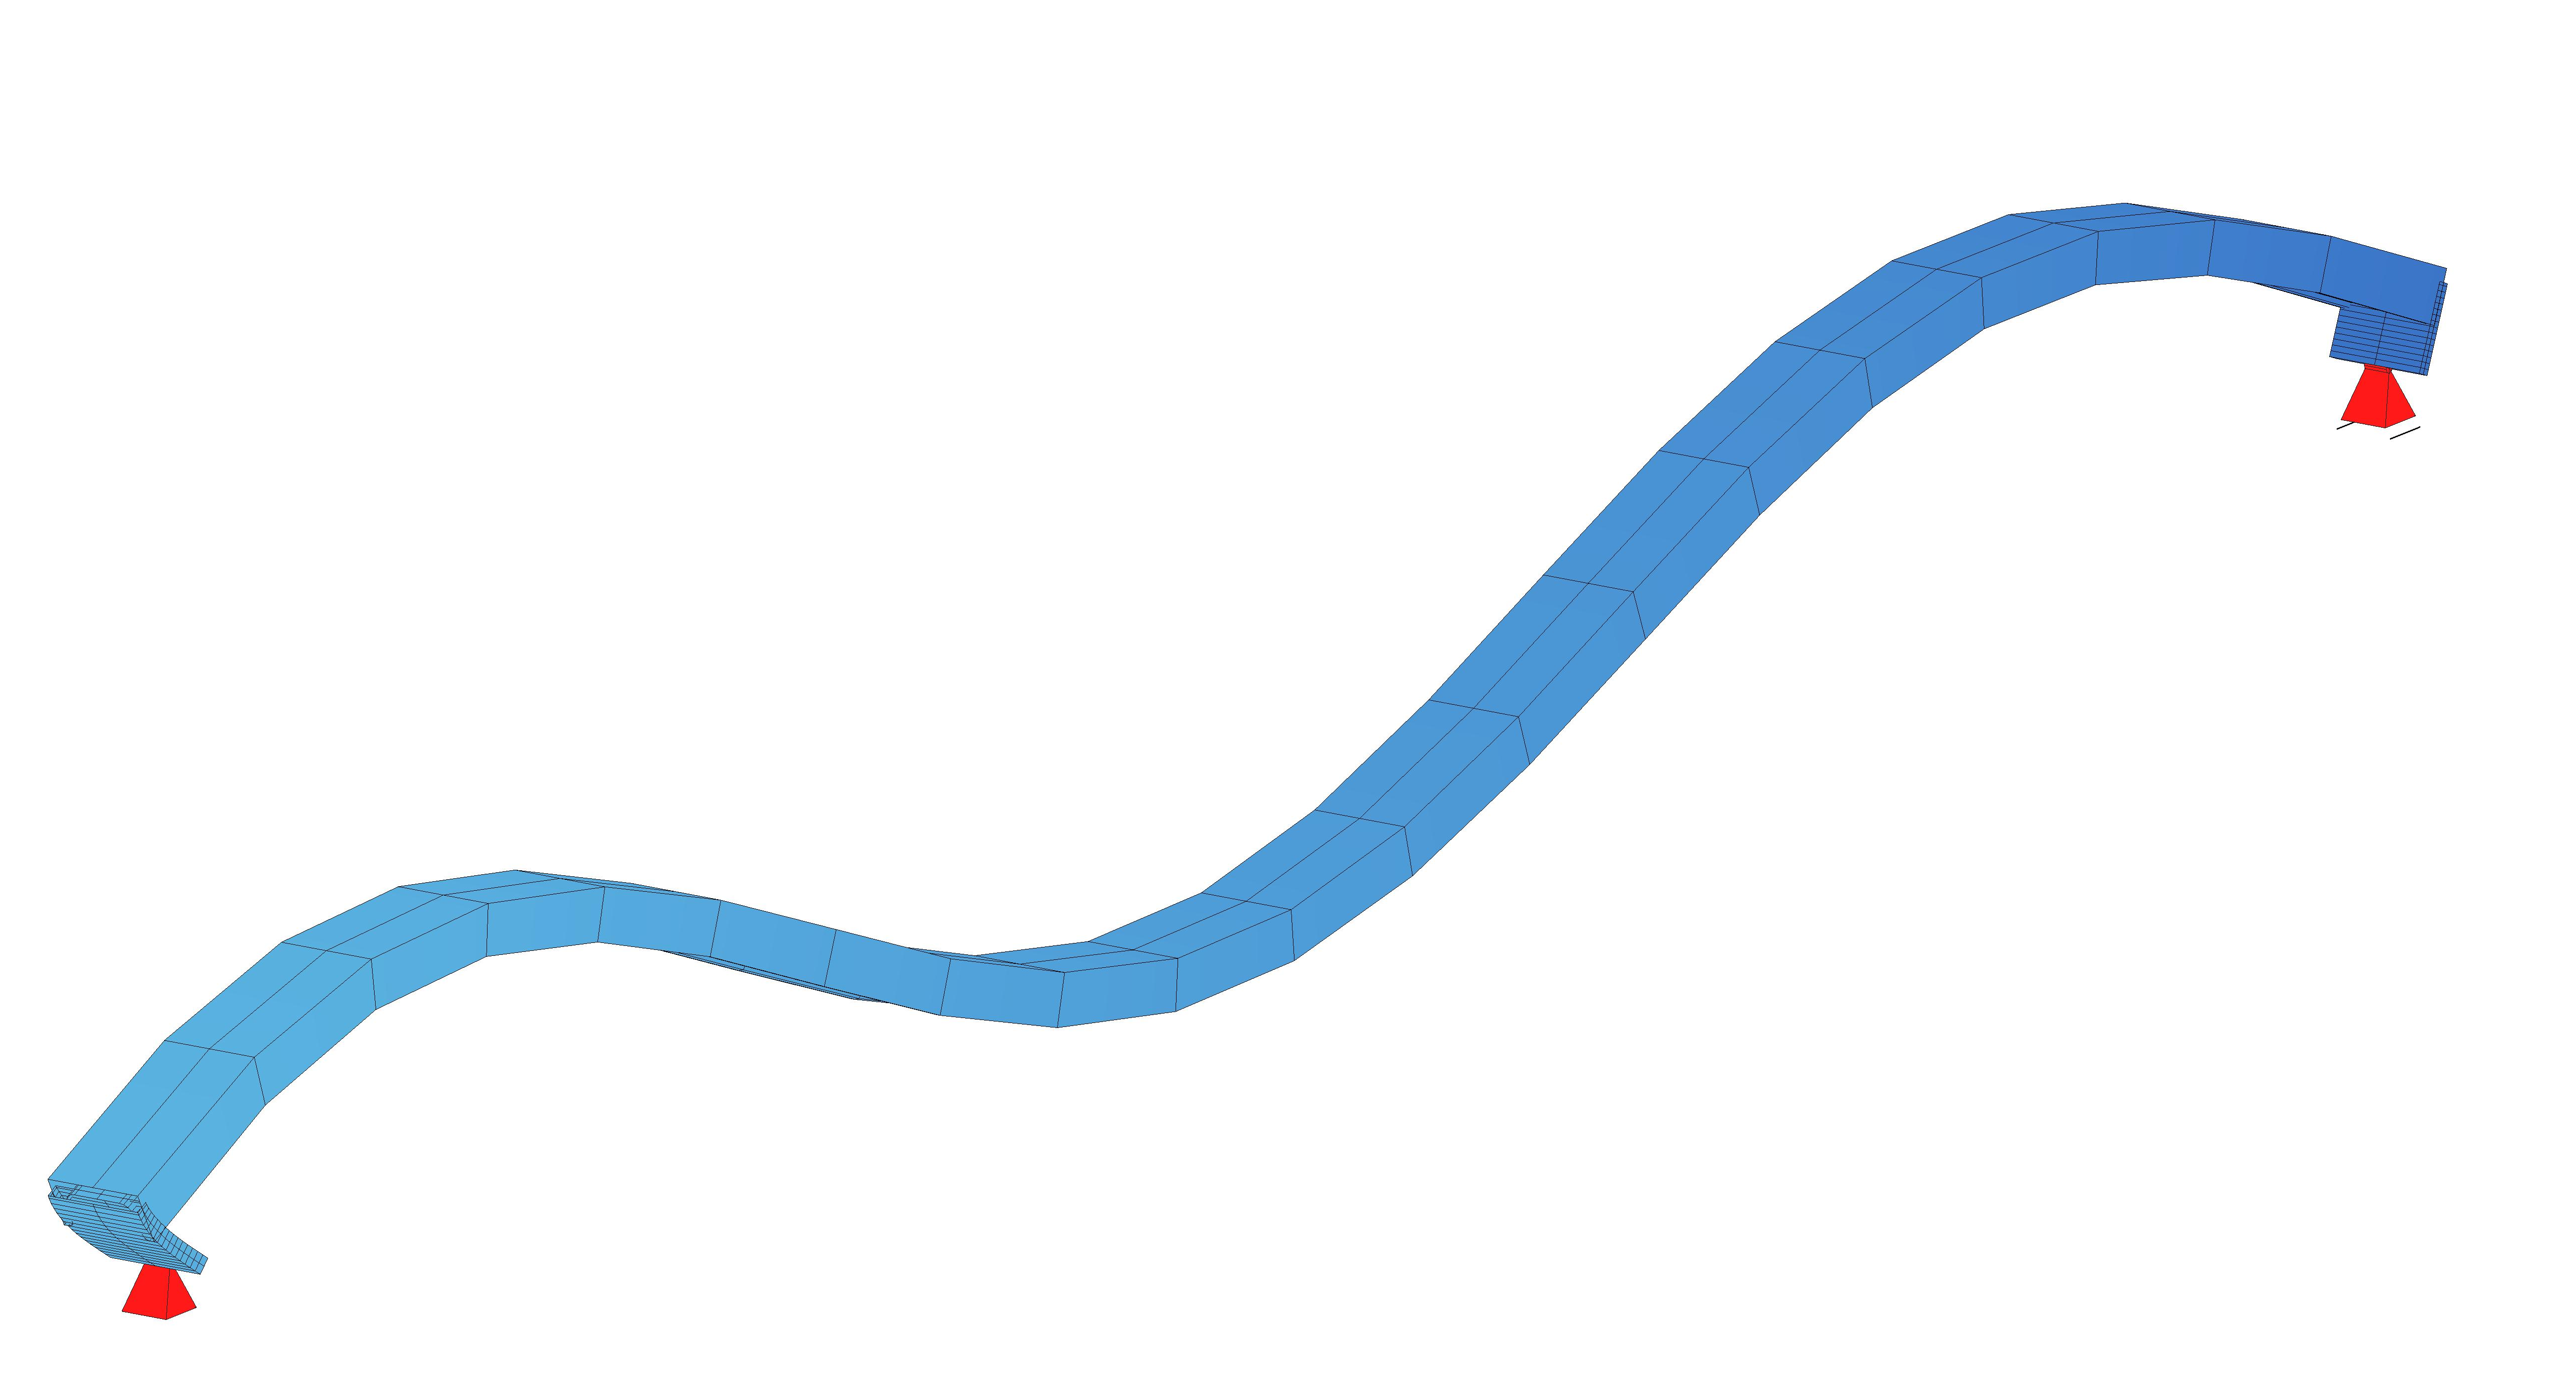
\includegraphics[width=0.33\linewidth]{/test_blue/sof_wis/image_small005.png}}%
	\subfloat[Mod 5, $f_5=200.38 \text{Hz}$]{\label{fig: test_blue_sof_mod5}%
		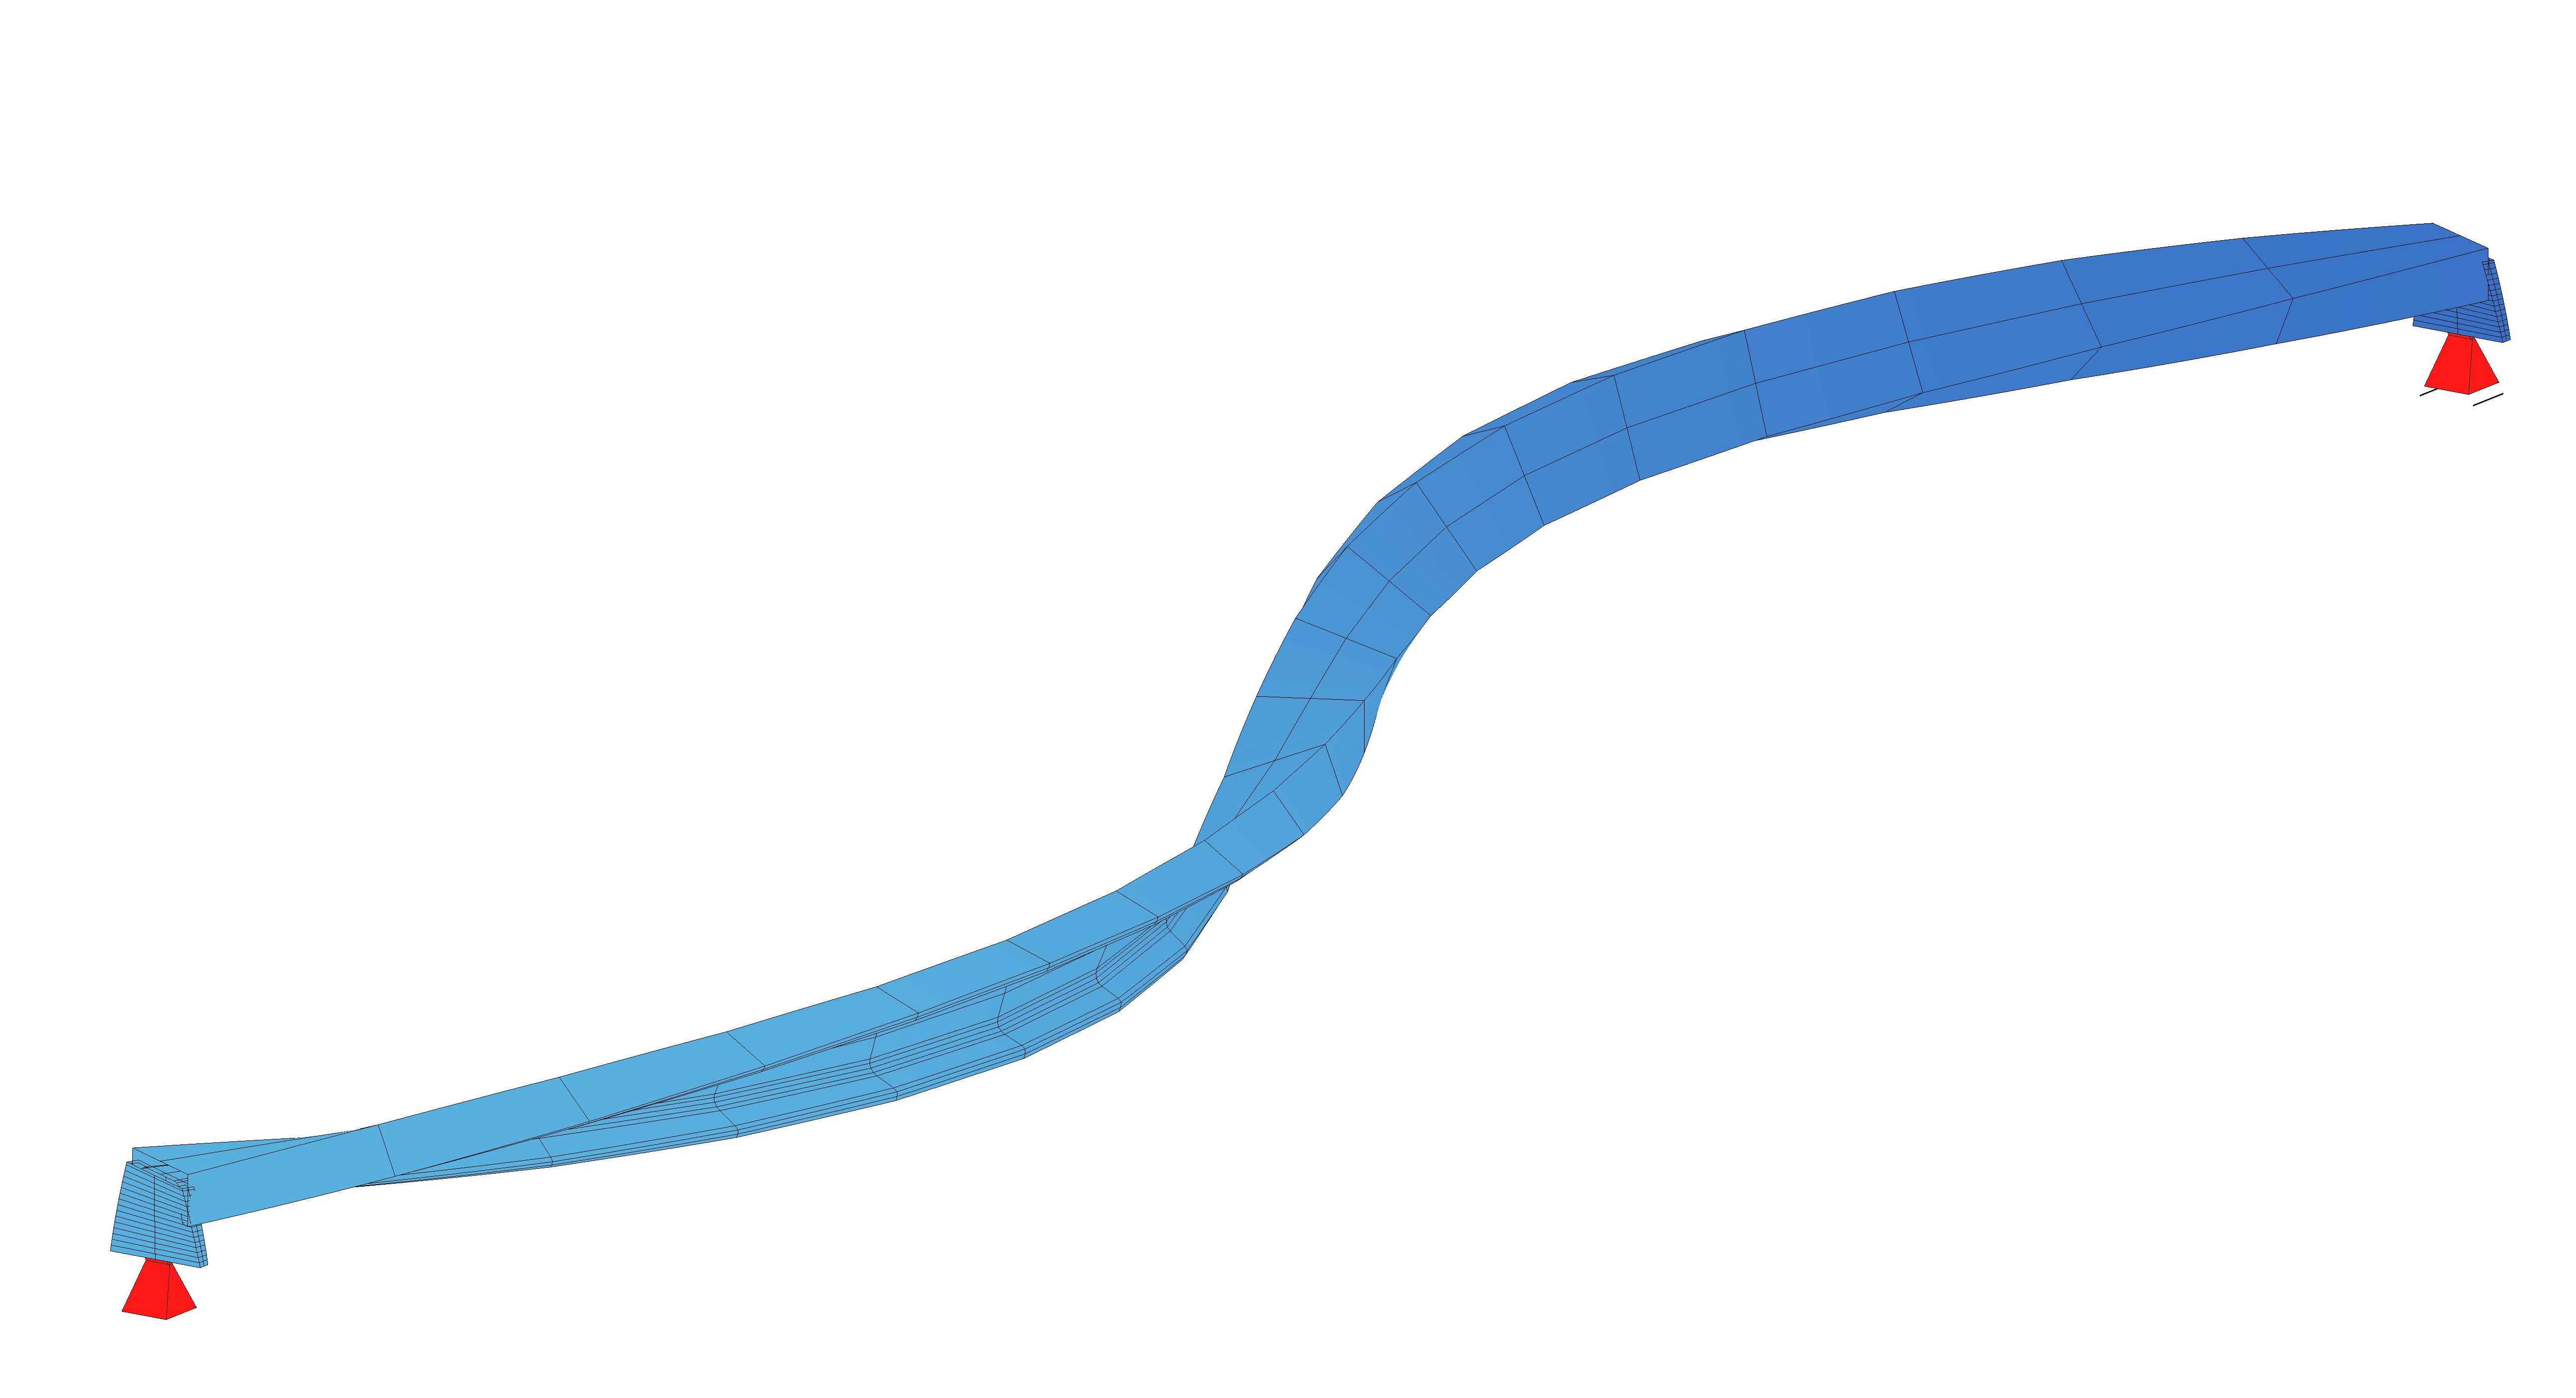
\includegraphics[width=0.33\linewidth]{/test_blue/sof_wis/image_small006.png}}%
	\subfloat[Mod 6, $f_6=212.24 \text{Hz}$]{\label{fig: test_blue_sof_mod6}%
		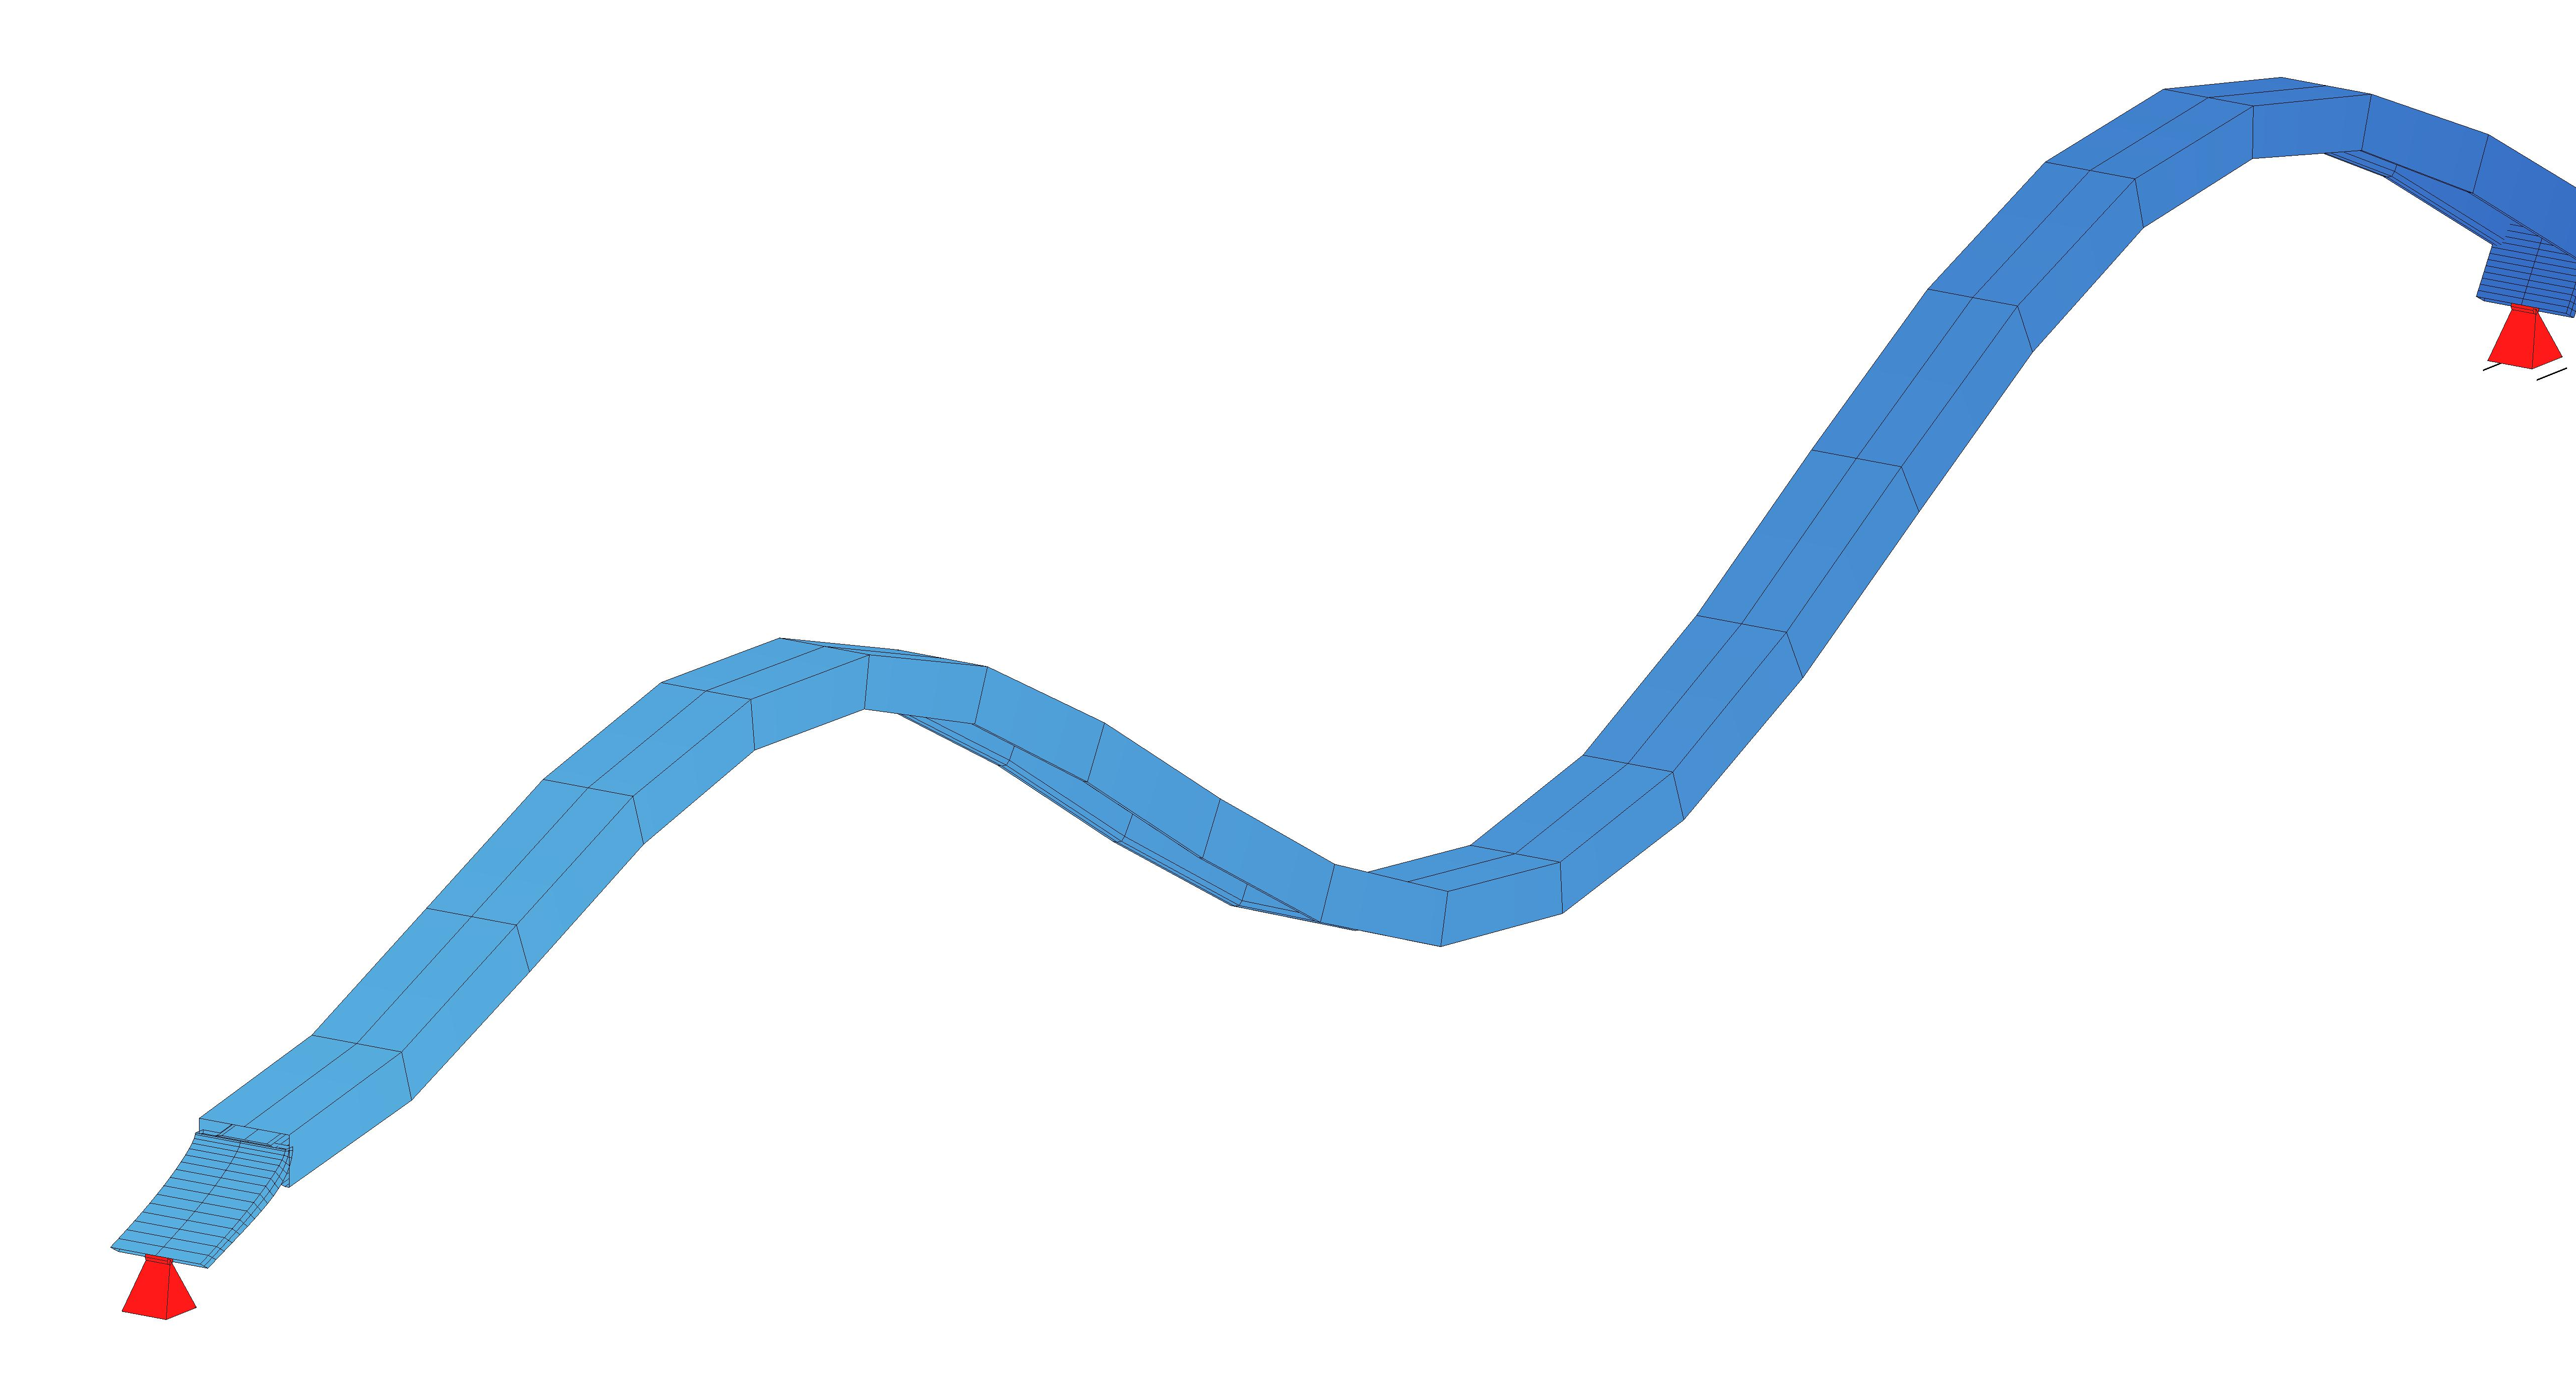
\includegraphics[width=0.33\linewidth]{/test_blue/sof_wis/image_small007.png}}\\
	\subfloat[Mod 7, $f_7=217.12 \text{Hz}$]{\label{fig: test_blue_sof_mod7}%
		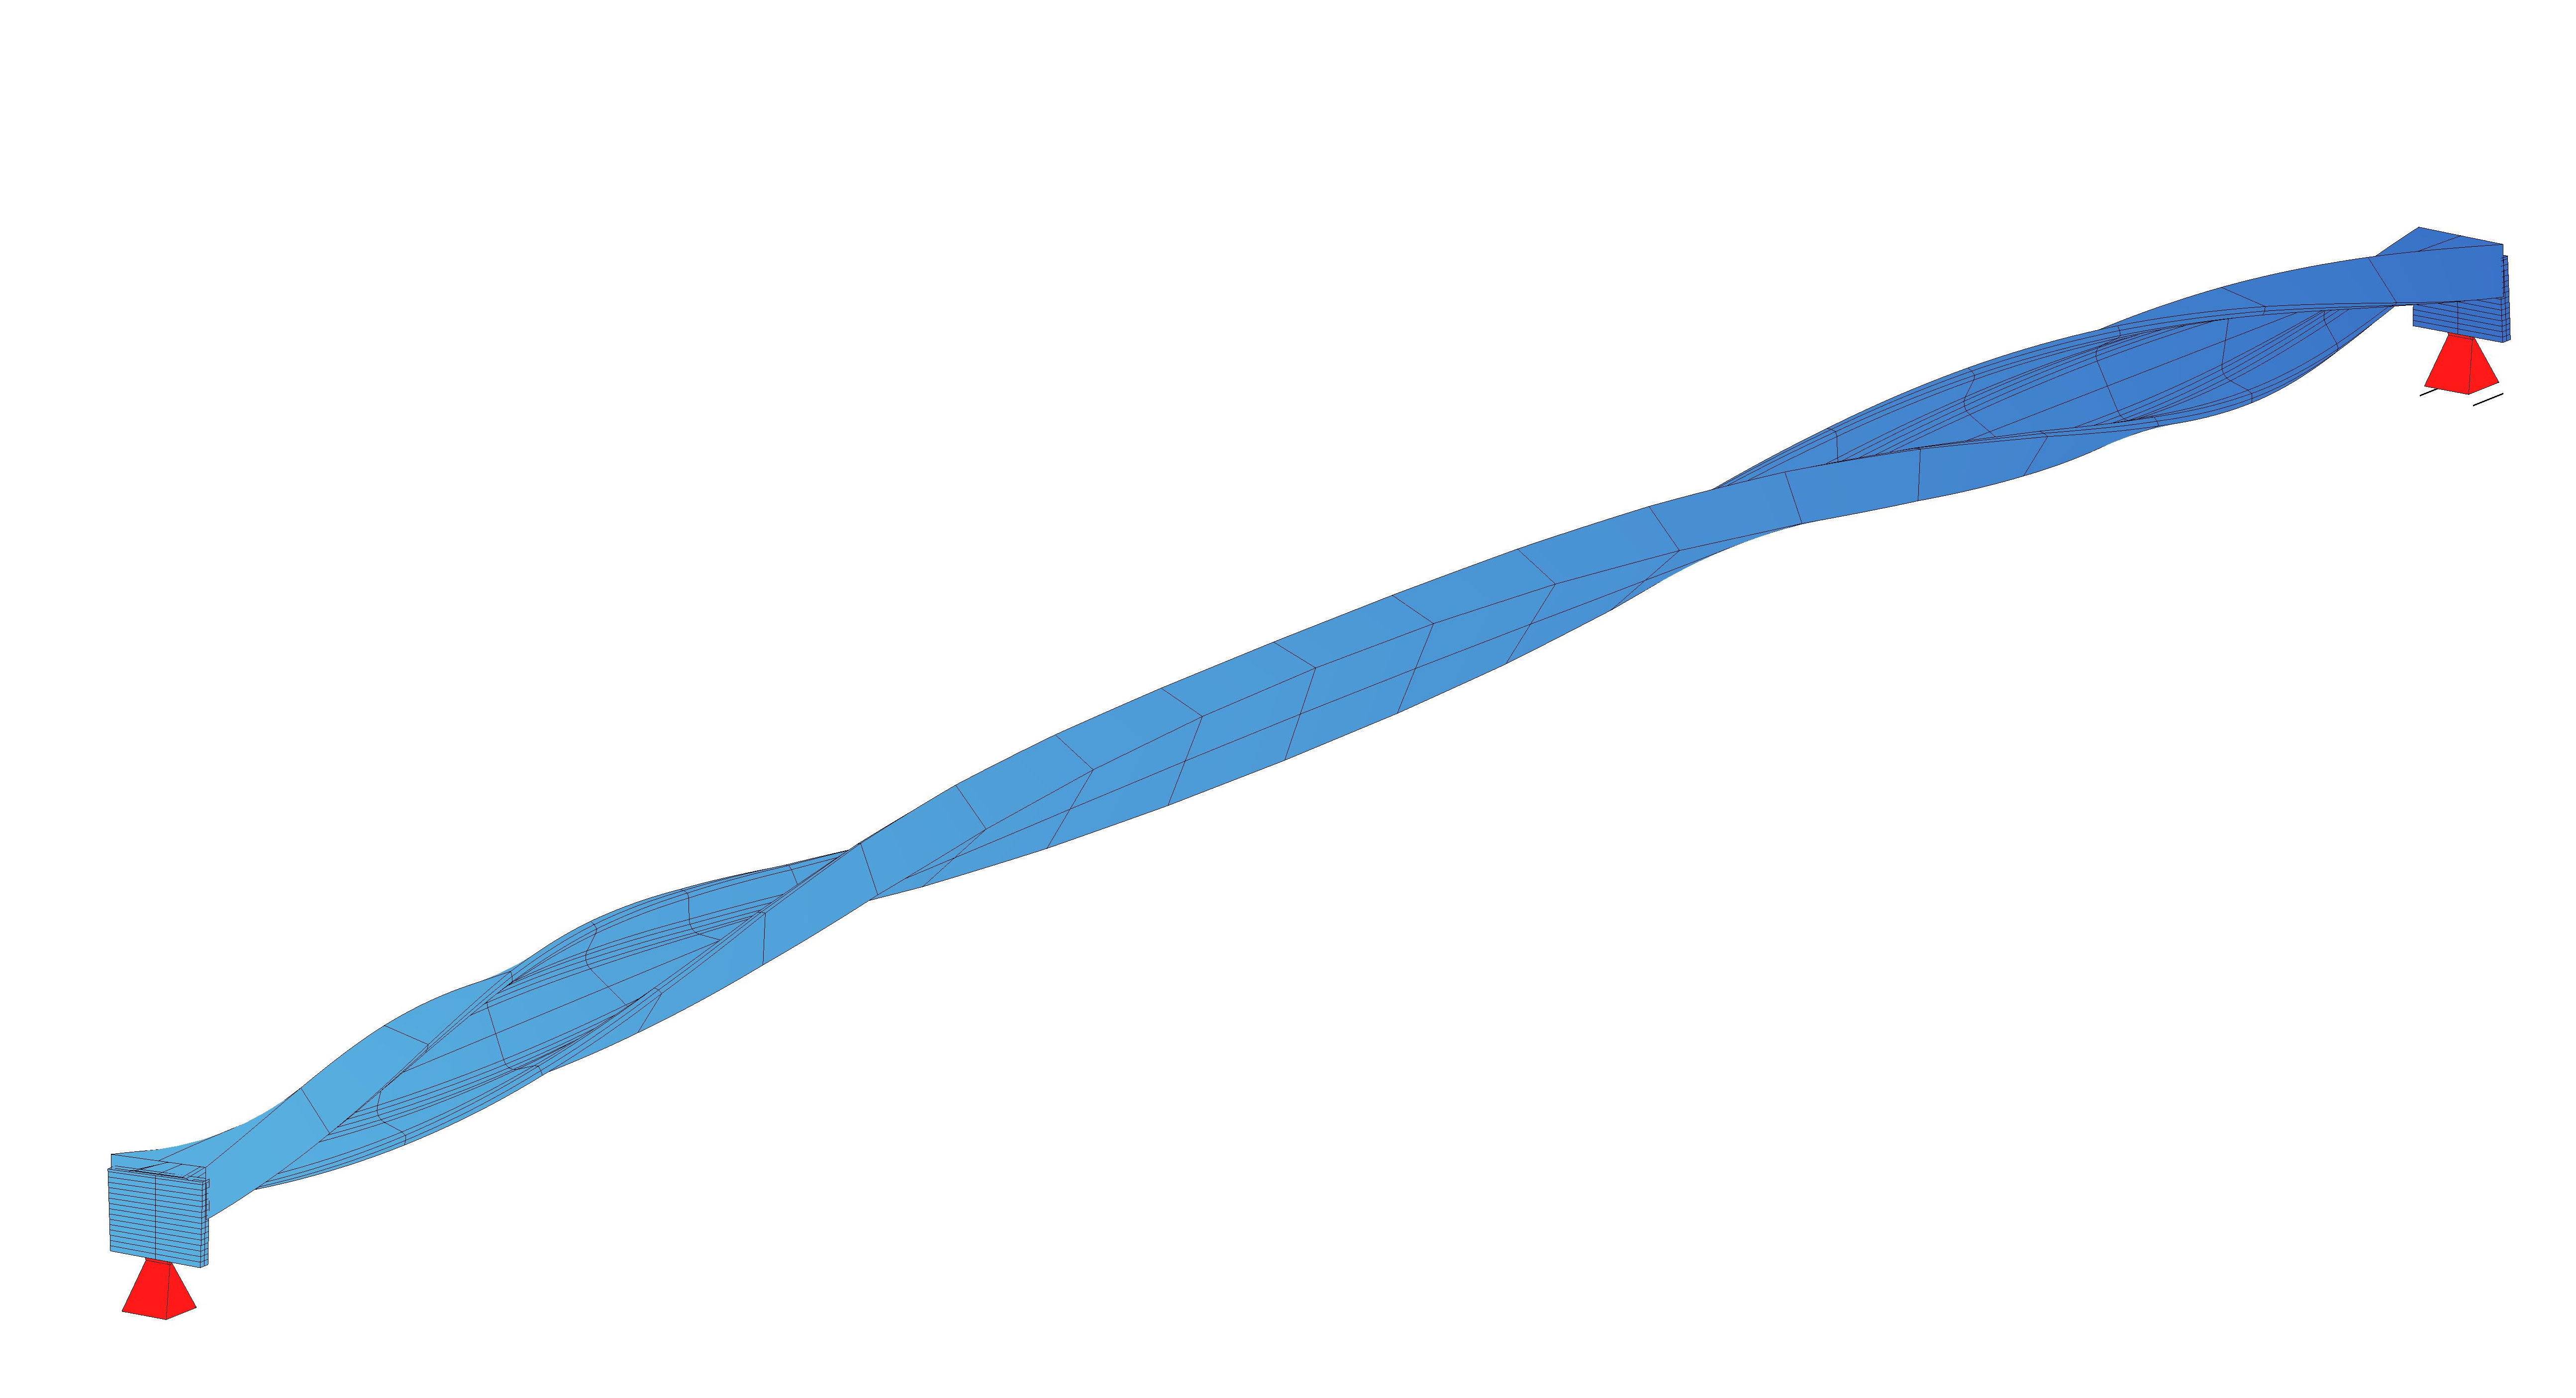
\includegraphics[width=0.33\linewidth]{/test_blue/sof_wis/image_small008.png}}%
	\subfloat[Mod 8, $f_8=336.59 \text{Hz}$]{\label{fig: test_blue_sof_mod8}%
		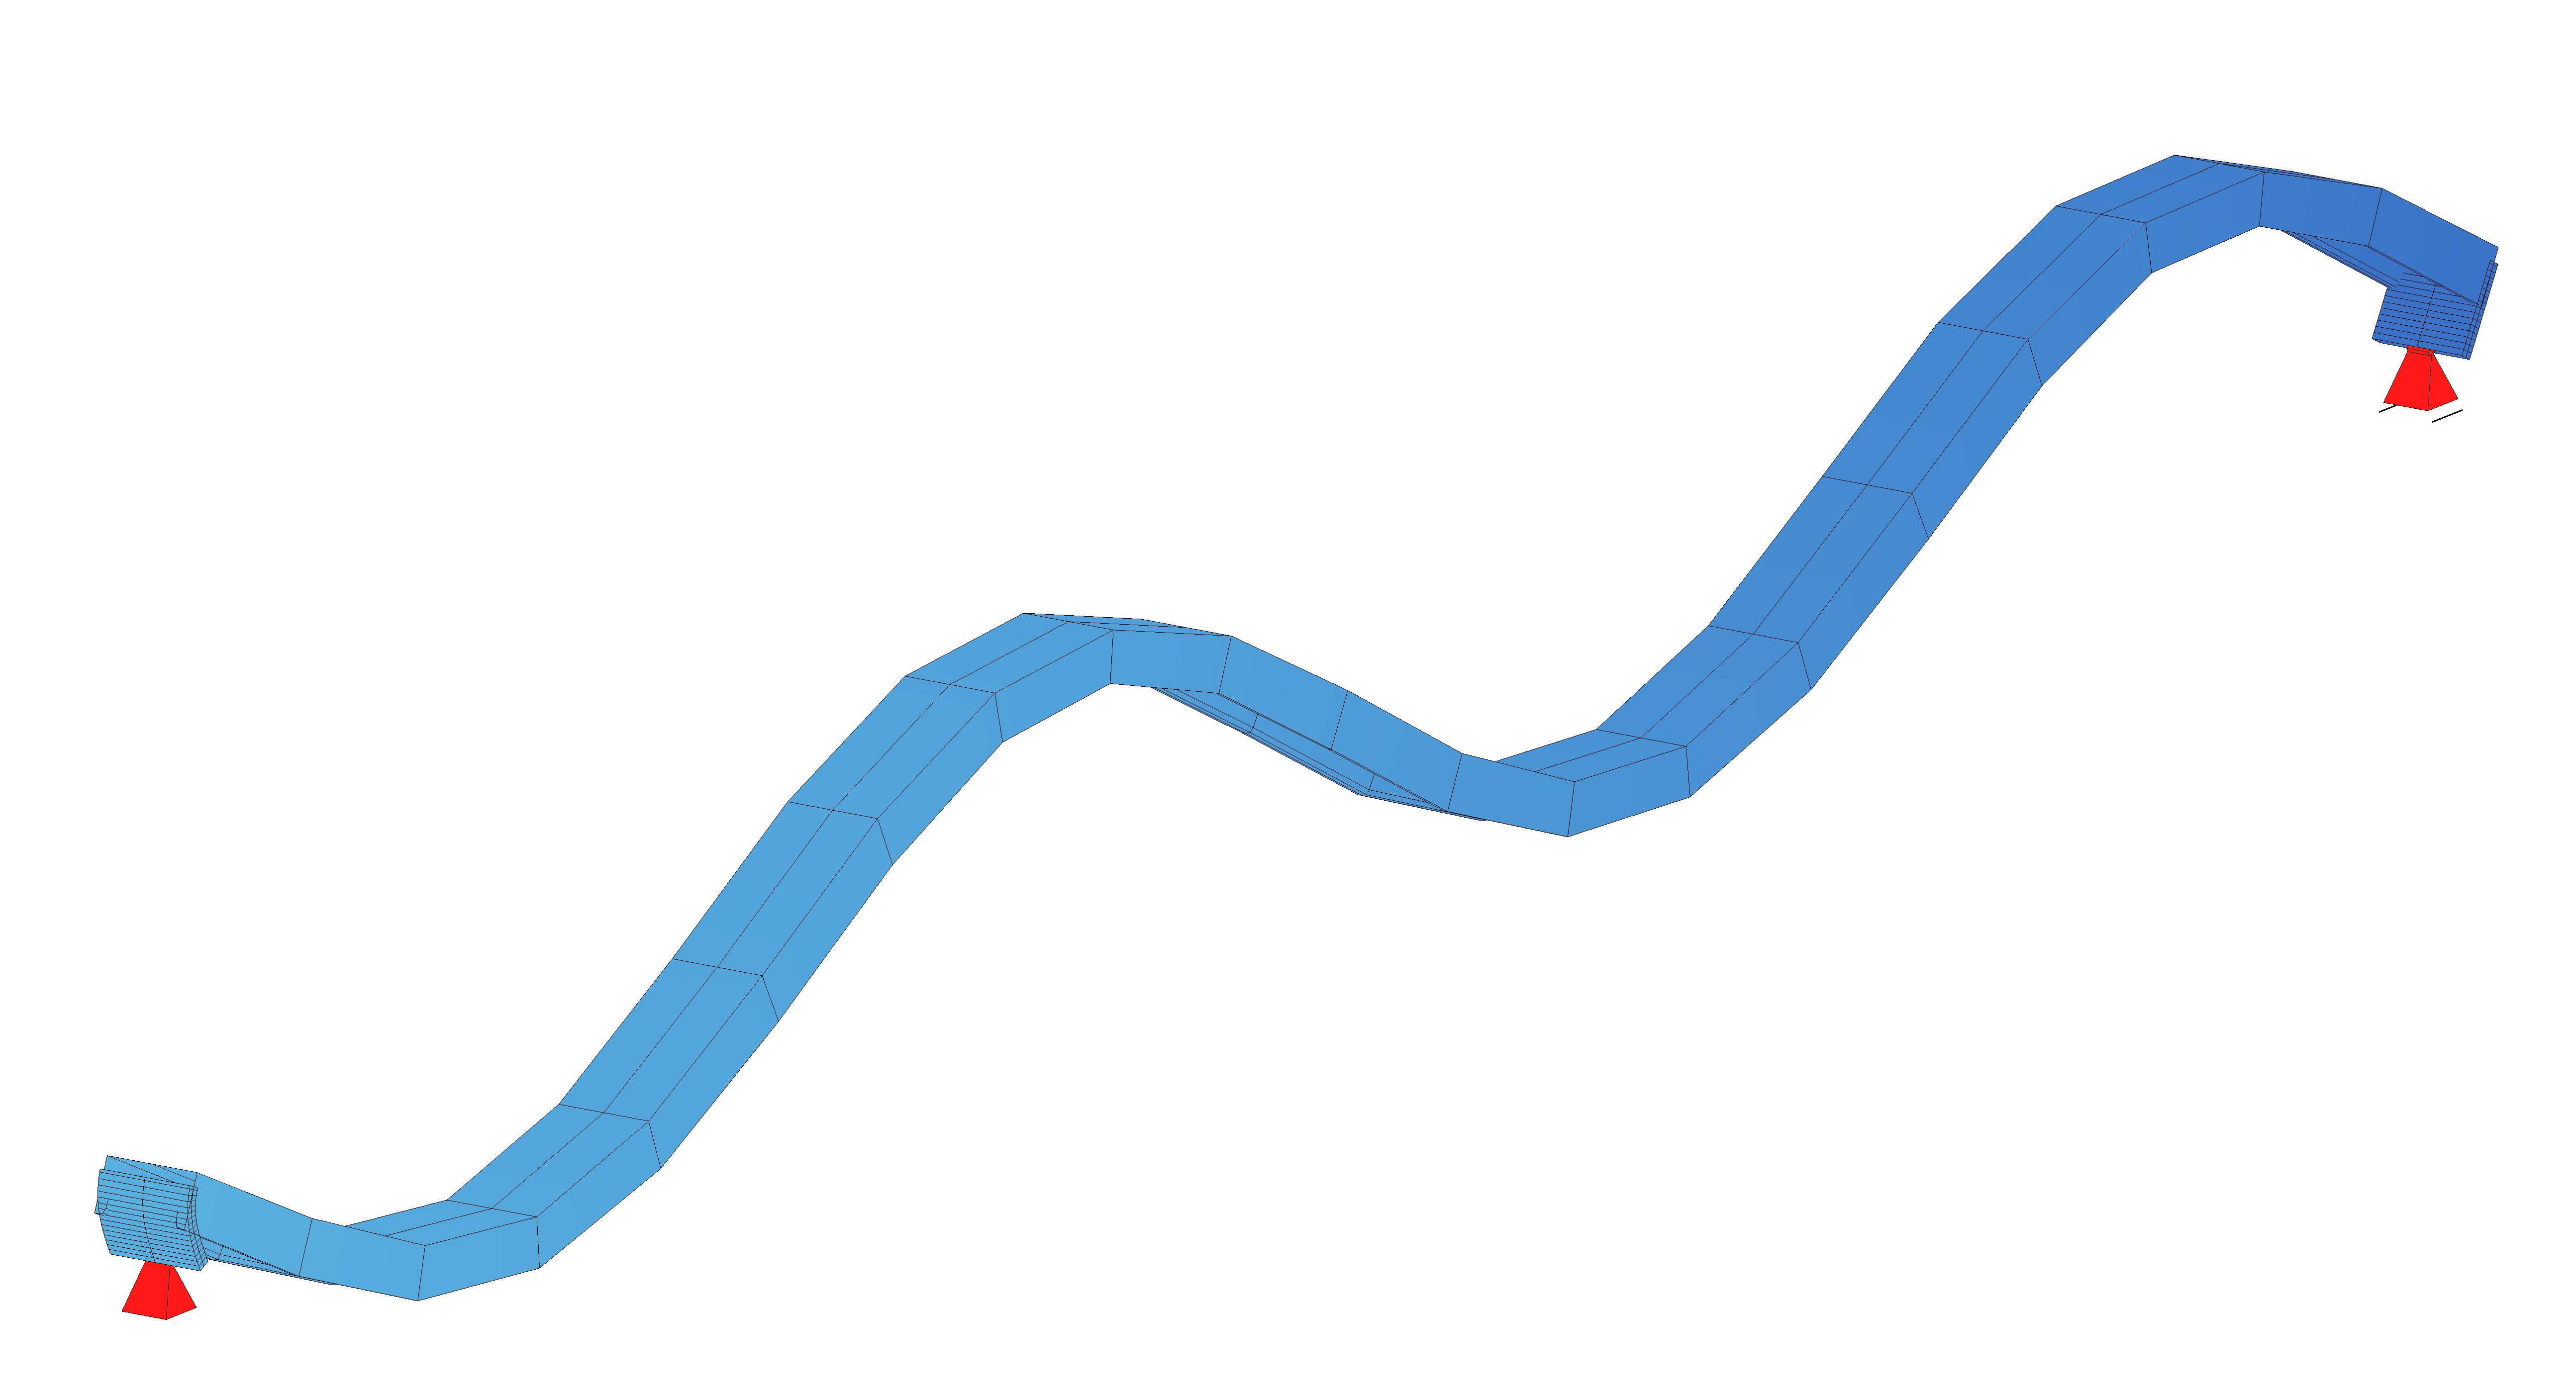
\includegraphics[width=0.33\linewidth]{/test_blue/sof_wis/image_small009.png}}%
	\subfloat[Mod 9, $f_9=410.22 \text{Hz}$]{\label{fig: test_blue_sof_mod9}%
		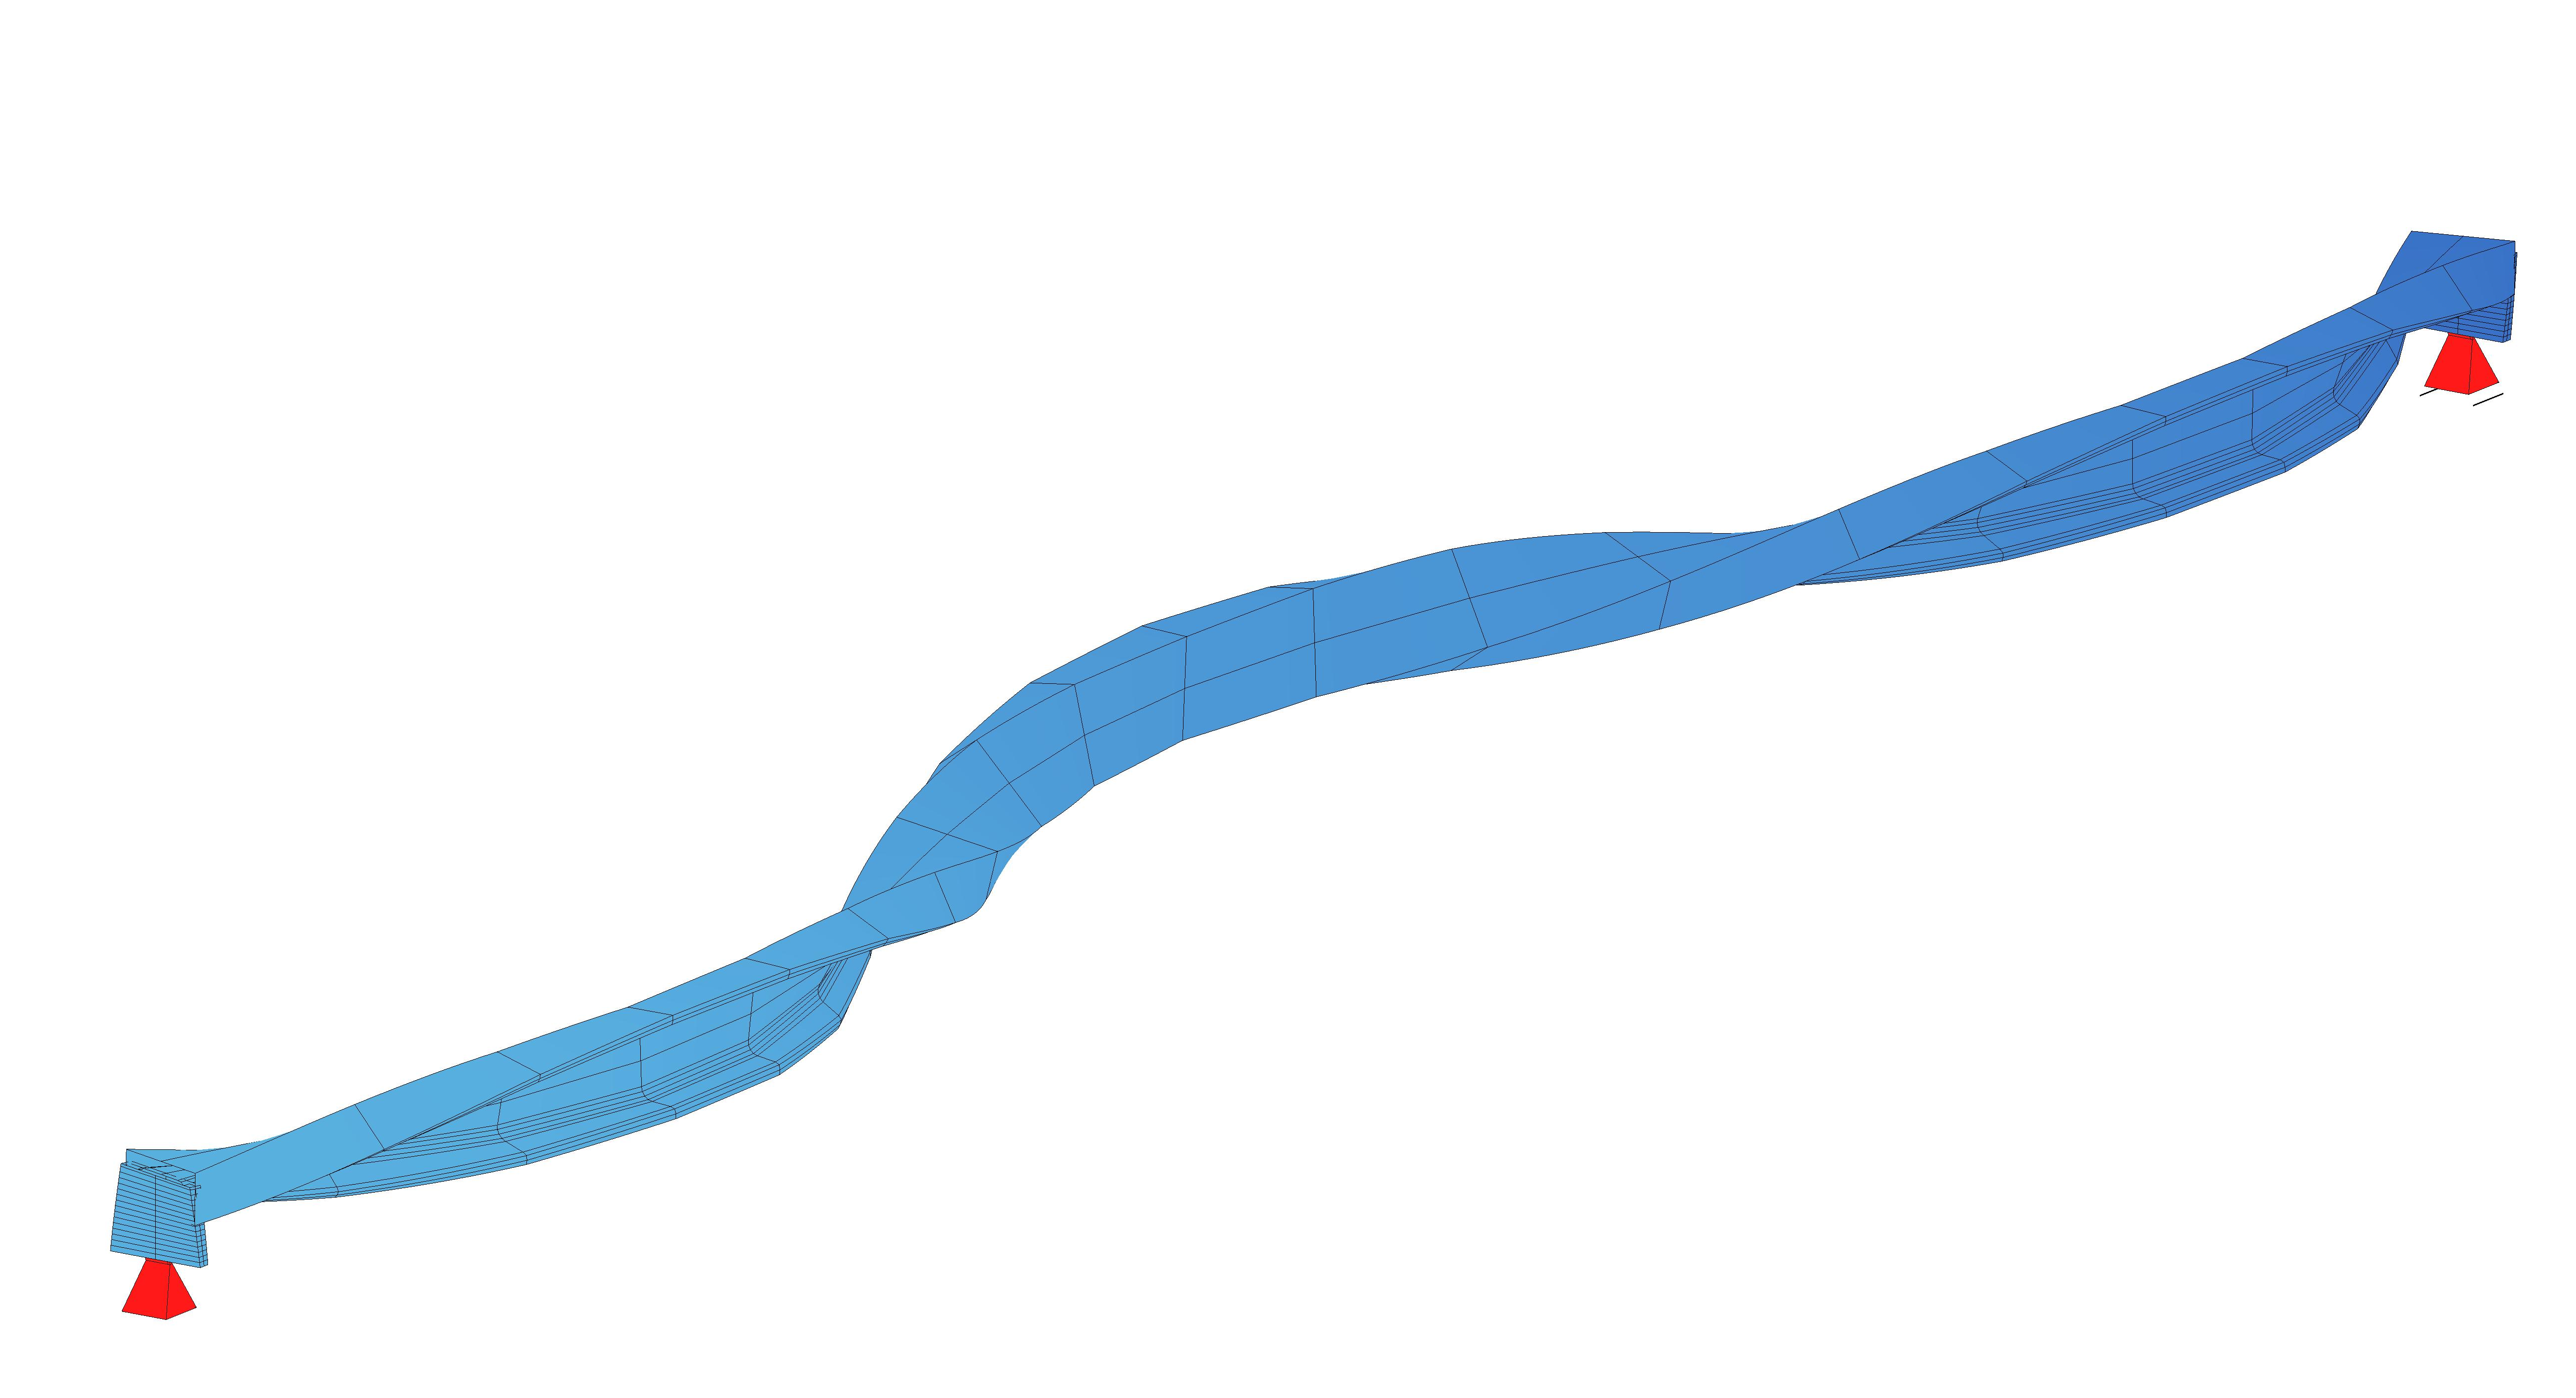
\includegraphics[width=0.33\linewidth]{/test_blue/sof_wis/image_small010.png}}\\
	\subfloat[Mod 10, $f_{10}=451.89 \text{Hz}$]{\label{fig: test_blue_sof_mod10}%
		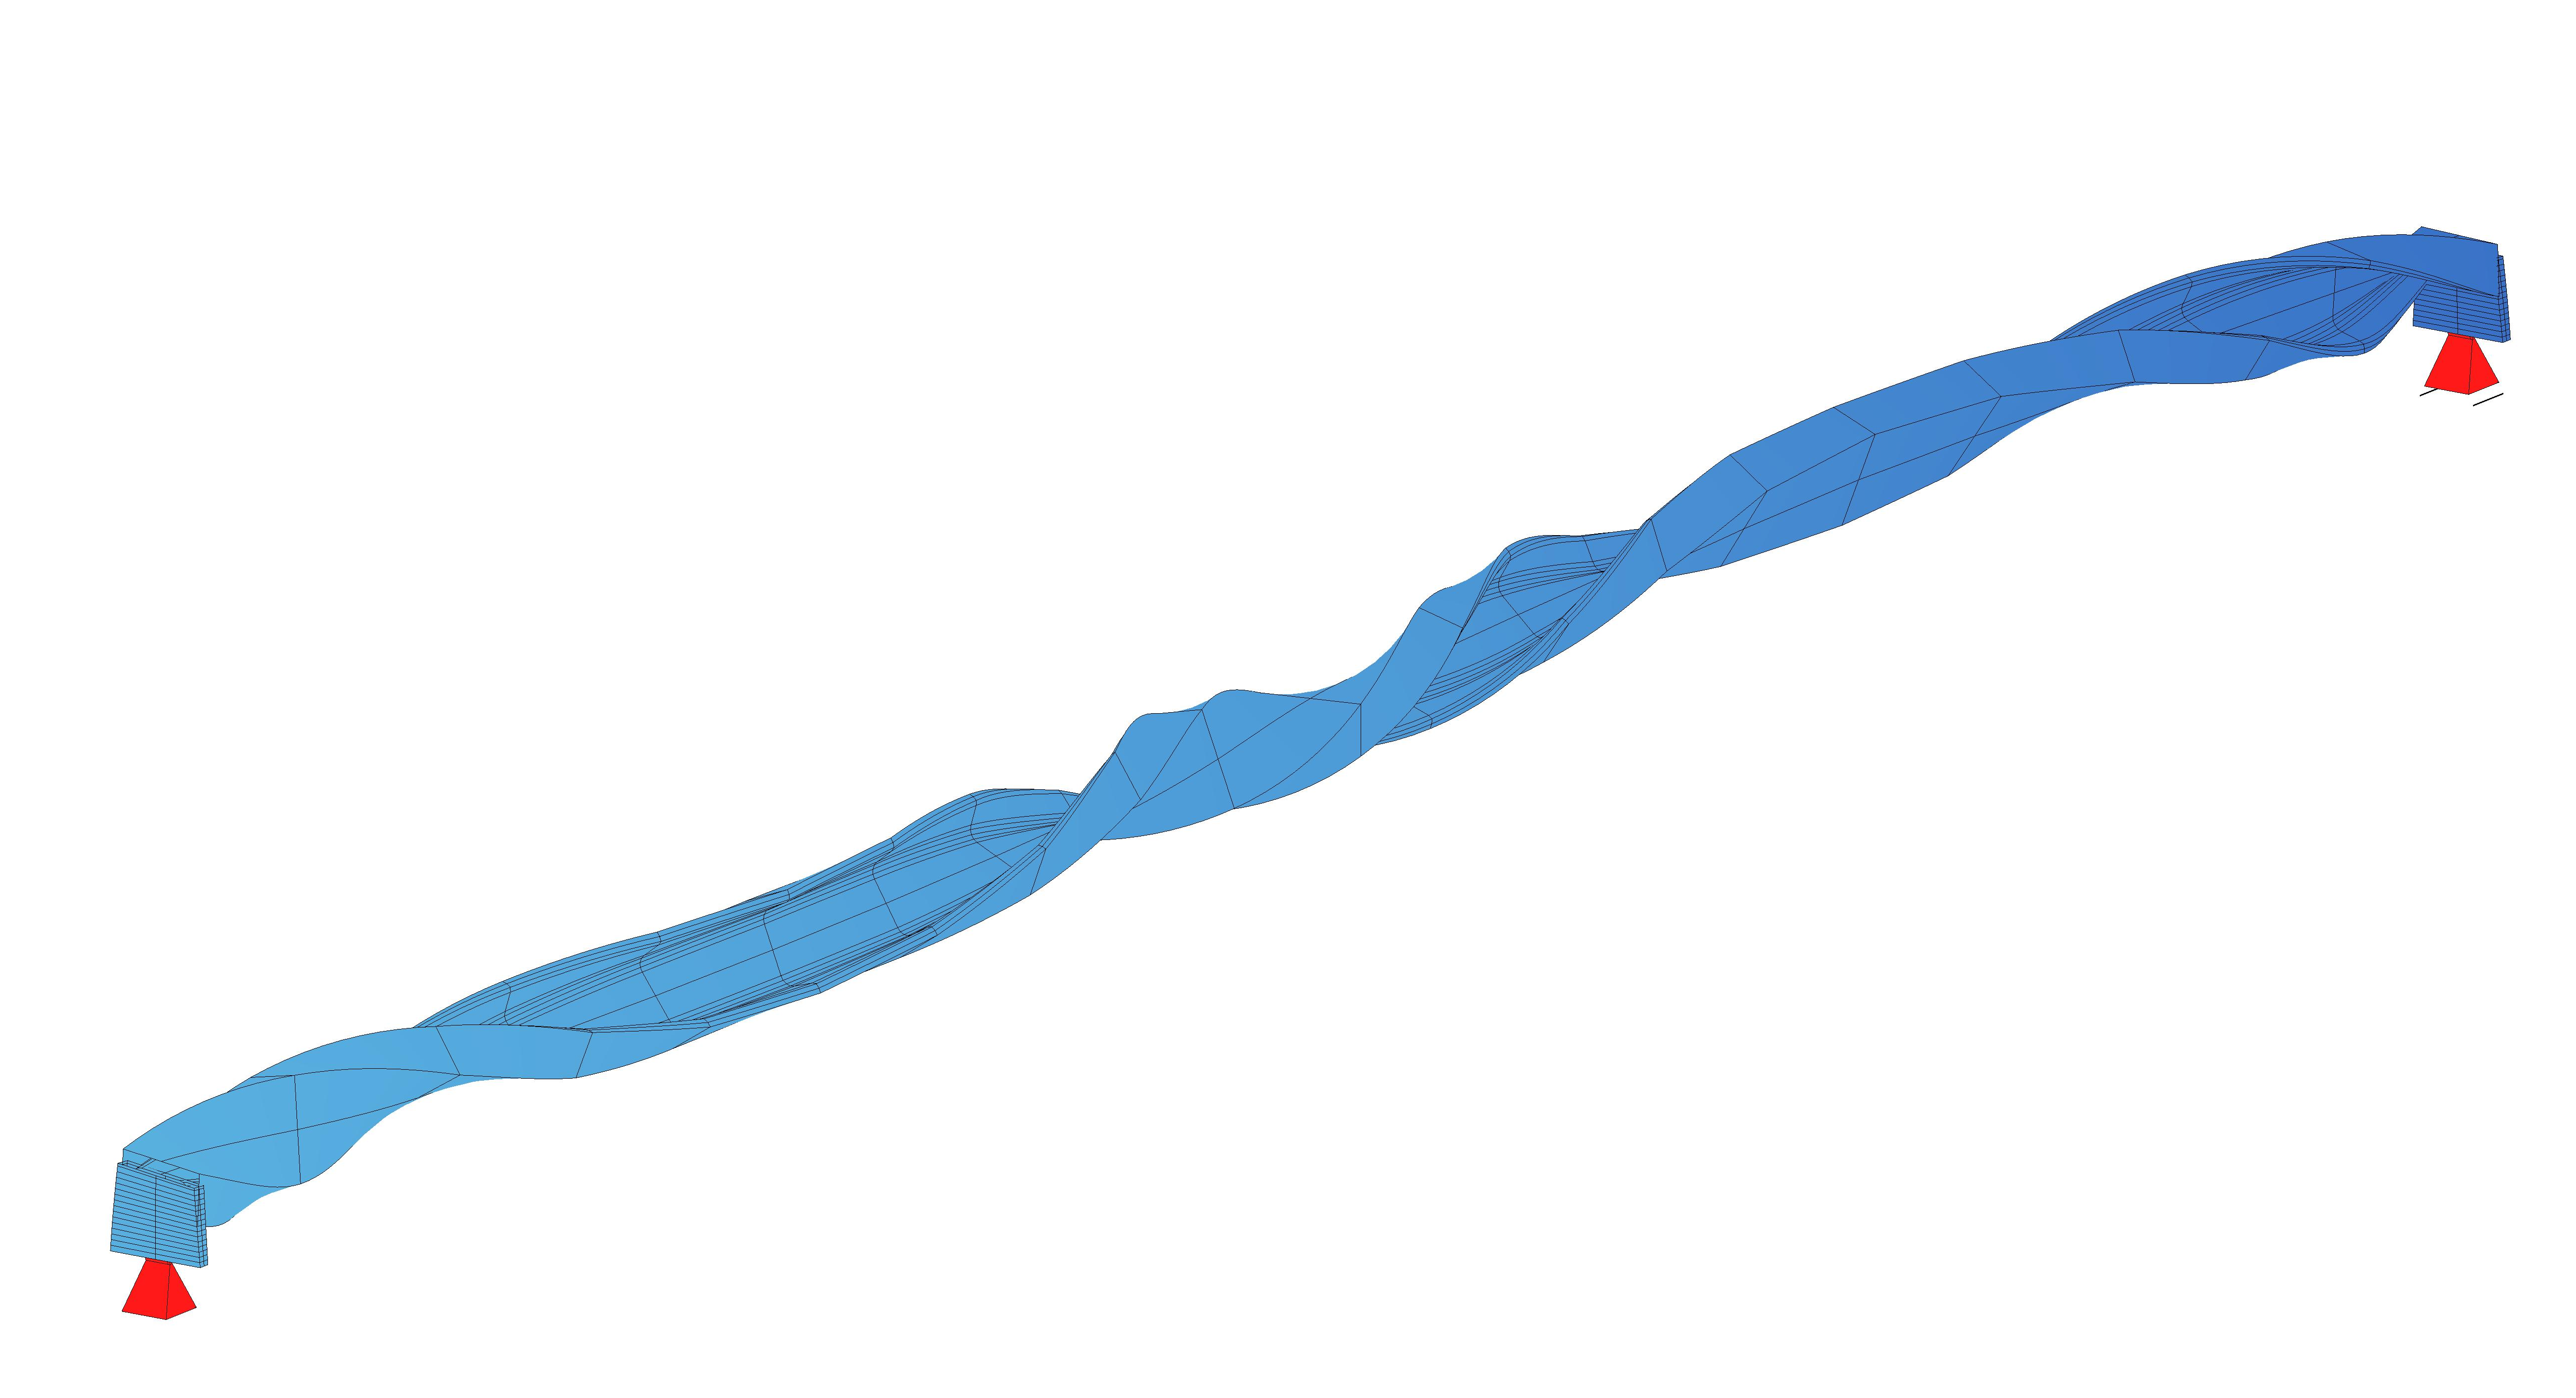
\includegraphics[width=0.33\linewidth]{/test_blue/sof_wis/image_small011.png}}\\
	
	\caption{Rozwiązanie analizy modalnej modelu testowego}
	\label{fig: modal_mods_blue_beam}
\end{figure}

Odpowiedź konstrukcji na wymuszenie losowe wyznaczono metodą time-step Newmarka-Wilsona. Zdecydowano o sprawdzeniu modów w zakresie do około 250Hz. Z tego względu przyjęto krok całkowania jako $\Delta t = 1/2500 s$. Zgodnie z kryterium Nyquista taki krok pozwala identyfikować drgania teoretycznie do częstotliwości 1250 Hz. Niemniej jednak, sygnał wyjściowy powinien zostać nadpróbkowany znacznie bardziej niżeli dwukrotnie. Aby zapewnić dokładność rezultatu, odpowiedź z rozwiązania numerycznego powinna być wyznaczona z próbkowaniem ok 10-15 razy większym niż częstotliwość najwyższego, interesującego modu \parencite{Kacprzyk1983,Rakowski2016,Bajer2012,Zotowski2017c}. Większość modów odczytanych z analizy modalnej mieści się w zamierzonym zakresie do 250 Hz. Kilka modów powyżej 250 Hz zostanie również uwzględnione w analizie dla pokazania zmniejszenia dokładności z uwagi na zbyt rzadkie próbkowanie. W każdym kroku struktura była obciążana losowym przypadkiem obliczeniowym z bazy 5000 wcześniej wygenerowanych. Tłumienie konstrukcji przyjęto jako masowo-sztywnościowe według metody Rayleigha (\ref{eq: rayleigh_damping}). Współczynniki metody wyznaczono zakładając tłumienie $\text{LDT}=3\%$ dla częstotliwości 20 Hz i 160 Hz. Chcąc sprawdzić charakter obciążenia wykonano analizę FFT sygnału złożonego z wartości obciążenia czterech węzłów w funkcji czasu. Widma częstotliwościowe przedstawiono na rysunku \ref{fig: fft_load_input_blue_beam}. Całkowity czas analizy przyjęto równy 25s ($25\cdot2500=62500$ kroków czasowych). Widmo częstotliwościowe nie ujawnia żadnej dominującej częstotliwości i można uznać je za równe w całym zakresie.
\begin{figure}[h]
	\centering
	\subfloat[Węzeł 7, kierunek Y]{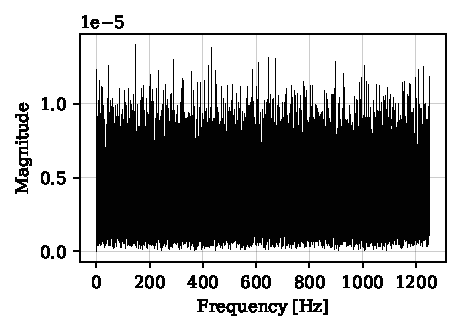
\includegraphics{/test_blue/input_load/input_load_1.pdf}}%
	\subfloat[Węzeł 7, kierunek Z]{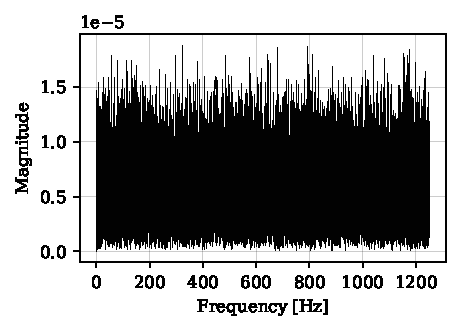
\includegraphics{/test_blue/input_load/input_load_2.pdf}}\\
	%\subfloat[Węzeł 11, kierunek Y]{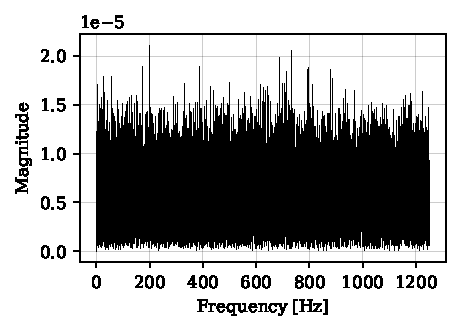
\includegraphics{/test_blue/input_load/input_load_3.pdf}}%
	%\subfloat[Węzeł 11, kierunek Z]{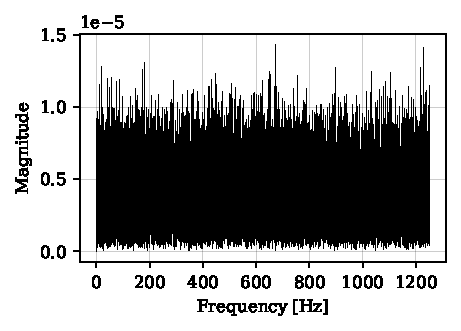
\includegraphics{/test_blue/input_load/input_load_4.pdf}}%
	\captionsetup{justification=centering}
	\caption{Transformaty Fouriera funkcji wymuszenia przykładowych węzłów w modelu testowym}
	\label{fig: fft_load_input_blue_beam}
\end{figure}

Dla obliczonego modelu odczytano przebieg przyspieszeń w dziewięciu węzłach pośrednich, na kierunku pionowym i poprzecznym. Do programu wprowadzono stworzone sygnały z informacją o lokalizacji punktów odczytu. Jako punkt referencyjny na kierunku $Y$ wybrano punkt odległy o 0.3L od podpory, a na kierunku pionowym $Z$ punkt odległy o 0.4L od podpory. O wyborze punktów referencyjnych decyduje warunek, że nie mogą one znajdować się w węzłach żadnej analizowanej postaci drgań. Doboru parametrów identyfikacji dokonano przy pomocy diagramu stabilizacyjnego (Rys. \ref{fig: stab_diags_blue_beam}). Na ostatecznym diagramie w wersji filtrowanej (Rys. \ref{fig: stab_diags_blue_beam_b}) wyraźnie widać 8 zidentyfikowanych, stabilnych modów. Odczytano minimalny rząd modelu zawierający wszystkie stabilne mody jako $n=20$. Diagram tworzony iteracyjnie pozwolił ostatecznie wyznaczyć parametry metody, które przynoszą pewne, stabilne rozwiązanie. Dobrane parametry użyto w celu wyznaczenia ostatecznego rozwiązania identyfikacji.

\begin{figure}[ht]
	\centering
	\subfloat[Diagram niefiltrowany]{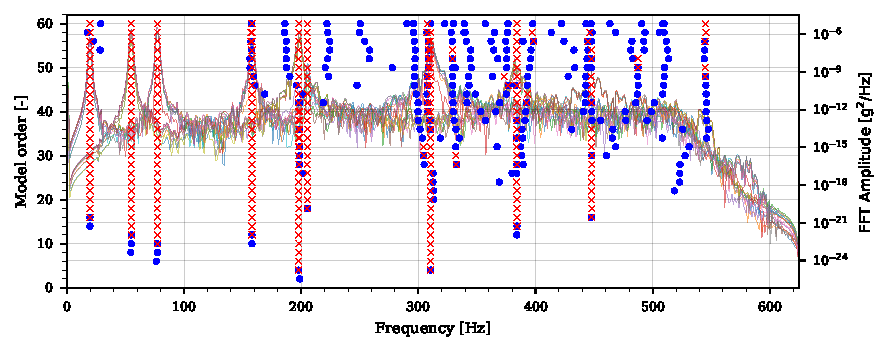
\includegraphics[width=\linewidth]{/test_blue/stab_diag/fig_stab_diagram_nonfiltr_time_20_20_50.pdf}}\\
	\subfloat[Diagram filtrowany]{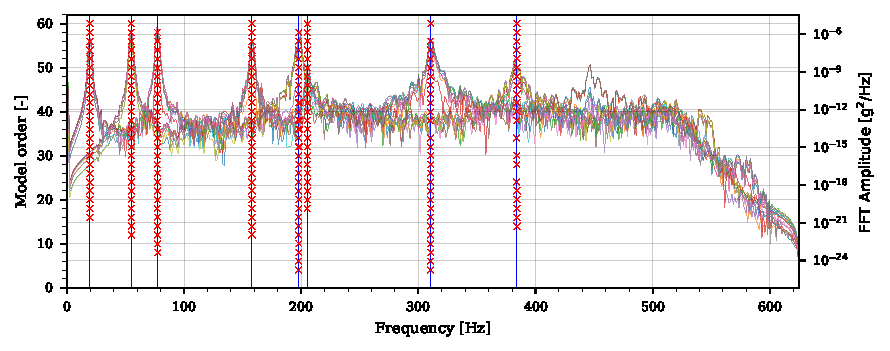
\includegraphics[width=\linewidth]{/test_blue/stab_diag/fig_stab_diagram_filtr_time_20_20_54.pdf},\label{fig: stab_diags_blue_beam_b}}%
	\captionsetup{justification=centering}
	\caption{Diagram stabilizacyjny metody NExT-ERA testowego modelu numerycznego: (a) diagram niefiltrowany, (b) diagram filtrowany}
	\label{fig: stab_diags_blue_beam}
\end{figure}

Wprowadzono wyznaczone parametry do programu. Uzyskano odpowiedzi impulsowe dla każdego punktu, których przykłady wraz z odpowiadającą im transformatą Fouriera przedstawiono na rysunku \ref{fig: cross_corr_blue_beam}. 

\begin{figure}[H]
	\centering
	\subfloat[Węzeł 7, kierunek Y]{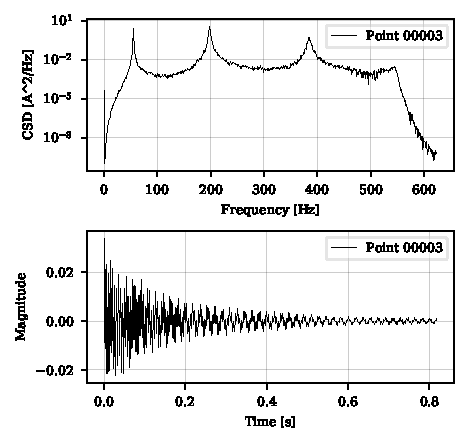
\includegraphics[width=0.5 \linewidth]{/test_blue/ccf/fig_CCF_CSD_00003_20_04_28.pdf}}%
	\subfloat[Węzeł 7, kierunek Z]{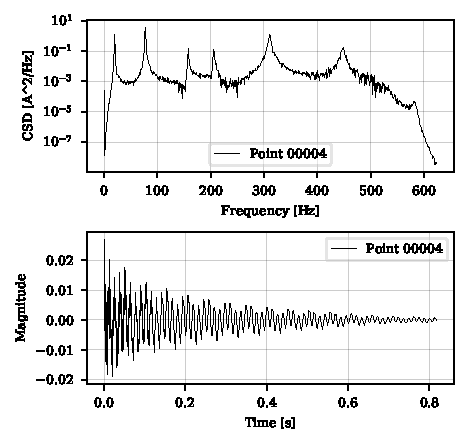
\includegraphics[width=0.5 \linewidth]{/test_blue/ccf/fig_CCF_CSD_00004_20_05_38.pdf}}\\
	\subfloat[Węzeł 11, kierunek Y]{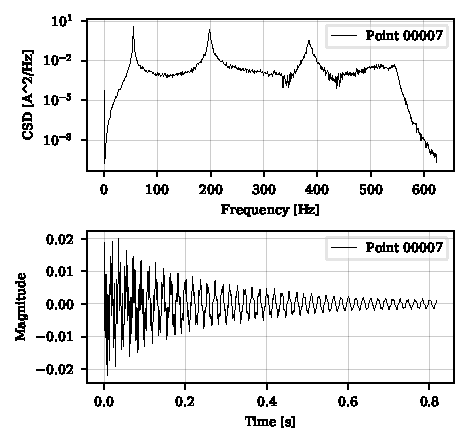
\includegraphics[width=0.5 \linewidth]{/test_blue/ccf/fig_CCF_CSD_00007_20_08_26.pdf}}%
	\subfloat[Węzeł 11, kierunek Z]{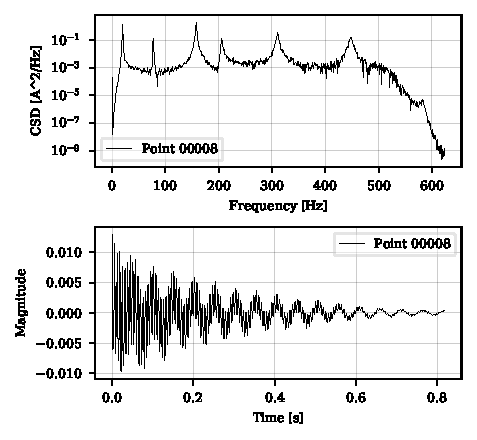
\includegraphics[width=0.5 \linewidth]{/test_blue/ccf/fig_CCF_CSD_00008_20_08_44.pdf}}%
	\captionsetup{justification=centering}
	\caption{Przykłady otrzymanych funkcji cross-korelacji w dziedzinie częstotliwości i dziedzinie czasu}
	\label{fig: cross_corr_blue_beam}
\end{figure}
Funkcje posiadają wyraźnie gasnący, okresowy charakter. Na odpowiadających im widmach zaznaczają się wyraźnie dominujące częstotliwości. Wyznaczone funkcje IRF zostały wprowadzone do metody ERA. Wyniki obliczono dla minimalnego rzędu modelu równego $n=20$ zgodnie ze wskazaniami diagramu stabilizacyjnego (Rys. \ref{fig: stab_diags_blue_beam}). Spośród wszystkich modów wybrano te, które na diagramie ujawniają się jako rzeczywiste i stabilne. Wyniki w formie postaci drgań własnych na kierunku pionowym $Z$ i poprzecznym $Y$ oraz dla obu kierunków w układzie biegunowym przedstawiono na rysunku \ref{fig: mods_blue_beam}. 

\begin{figure}[p]
	\centering
	\begin{tabular}[c]{c}
		\subfloat[Mod 1, $f_1=19.701 \text{Hz}$]{\label{fig: test_blue_mod1}%
			\begin{tabular}[b]{c c c}
				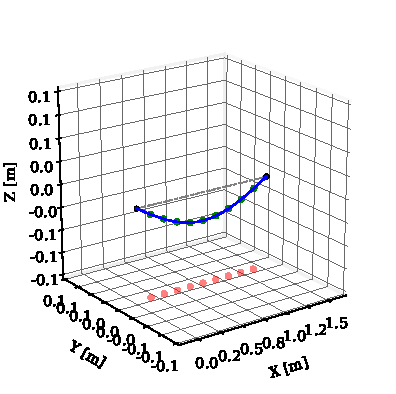
\includegraphics[width=0.35\linewidth]{/test_blue/blue_modes/fig_mod_0_time_22_08_38.pdf}%
				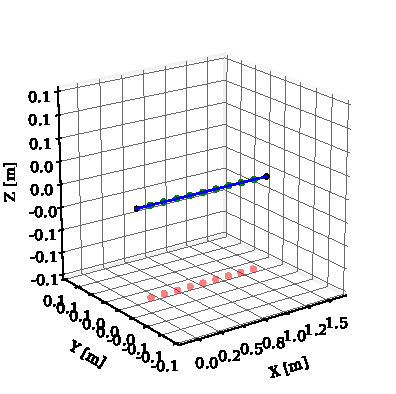
\includegraphics[width=0.35\linewidth]{/test_blue/blue_modes/fig_mod_0_time_22_08_55.pdf}%
				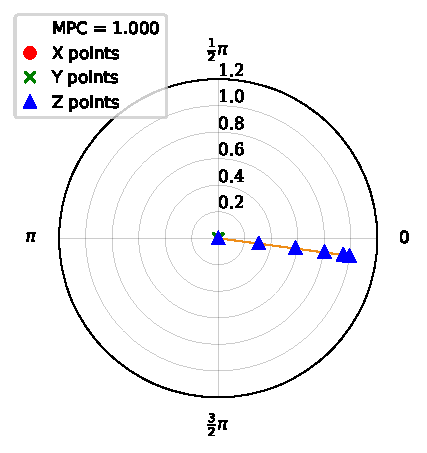
\includegraphics[width=0.3\linewidth]{/test_blue/polar/fig_polar_mod_0_time_22_07_54.pdf}%
		\end{tabular}}\\
		
		\subfloat[Mod 2, $f_2=54.958 \text{Hz}$]{\label{fig: test_blue_mod2}%
			\begin{tabular}[b]{c c}
				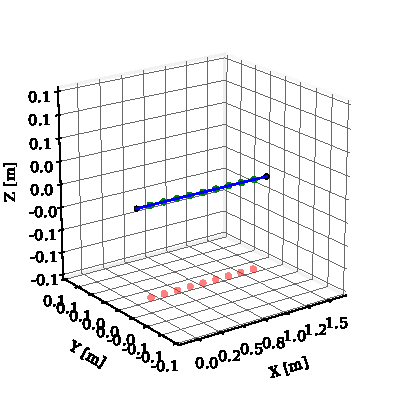
\includegraphics[width=0.35\linewidth]{/test_blue/blue_modes/fig_mod_2_time_22_09_15.pdf}%
				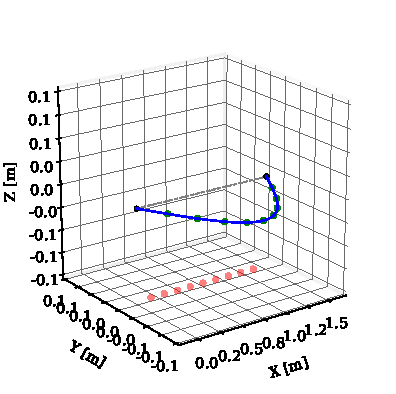
\includegraphics[width=0.35\linewidth]{/test_blue/blue_modes/fig_mod_2_time_22_09_26.pdf}%
				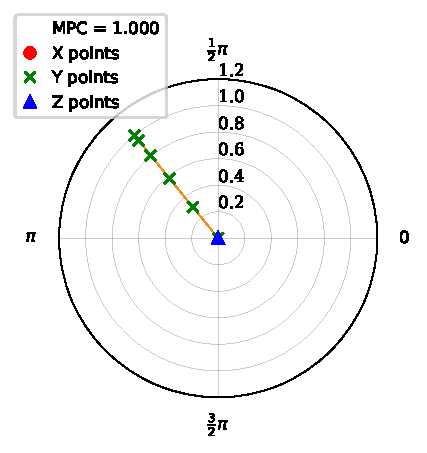
\includegraphics[width=0.3\linewidth]{/test_blue/polar/fig_polar_mod_2_time_22_09_04.pdf}%
		\end{tabular}}\\
		\subfloat[Mod 3, $f_3=77.331 \text{Hz}$]{\label{fig: test_blue_mod3}%
			\begin{tabular}[b]{c c}
				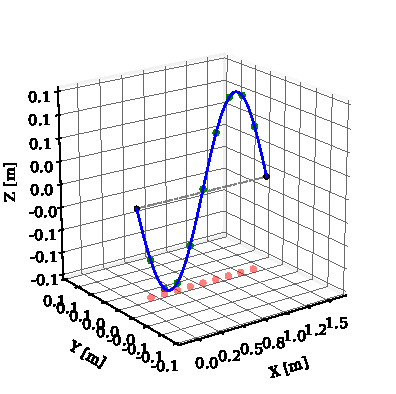
\includegraphics[width=0.35\linewidth]{/test_blue/blue_modes/fig_mod_4_time_22_09_56.pdf}%
				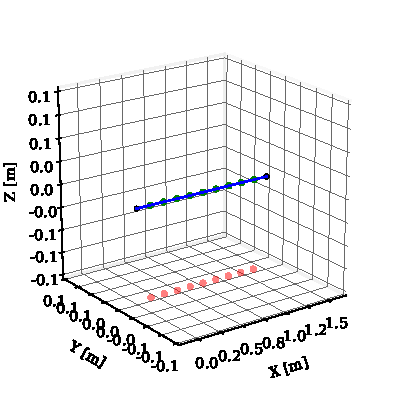
\includegraphics[width=0.35\linewidth]{/test_blue/blue_modes/fig_mod_4_time_22_10_36.pdf}%
				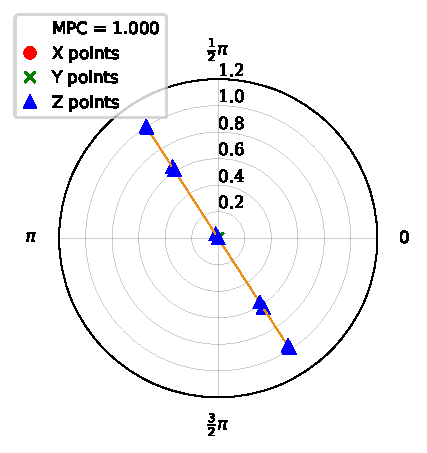
\includegraphics[width=0.3\linewidth]{/test_blue/polar/fig_polar_mod_4_time_22_09_47.pdf}%
		\end{tabular}}\\
		\subfloat[Mod 4, $f_4=157.995 \text{Hz}$]{\label{fig: test_blue_mod4}%
			\begin{tabular}[b]{c c}
				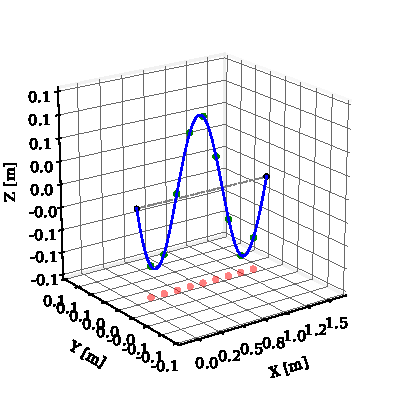
\includegraphics[width=0.35\linewidth]{/test_blue/blue_modes/fig_mod_6_time_22_10_59.pdf}%
				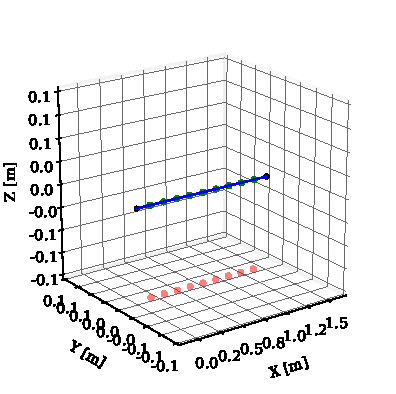
\includegraphics[width=0.35\linewidth]{/test_blue/blue_modes/fig_mod_6_time_22_11_12.pdf}%
				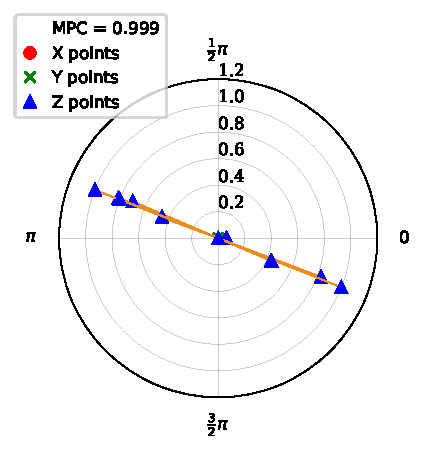
\includegraphics[width=0.3\linewidth]{/test_blue/polar/fig_polar_mod_6_time_22_10_52.pdf}%
		\end{tabular}}\\
	\end{tabular}
	\caption{Zidentyfikowane charakterystyki modalne belki testowej}
	\label{fig: mods_blue_beam}
\end{figure}

\begin{figure}[p]\ContinuedFloat
	\centering
	\begin{tabular}[c]{c}
		\subfloat[Mod 5, $f_5=197.881 \text{Hz}$]{\label{fig: test_blue_mod5}%
			\begin{tabular}[b]{c c c}
				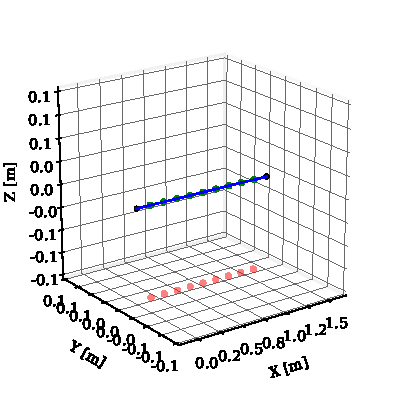
\includegraphics[width=0.35\linewidth]{/test_blue/blue_modes/fig_mod_8_time_22_11_37.pdf}%
				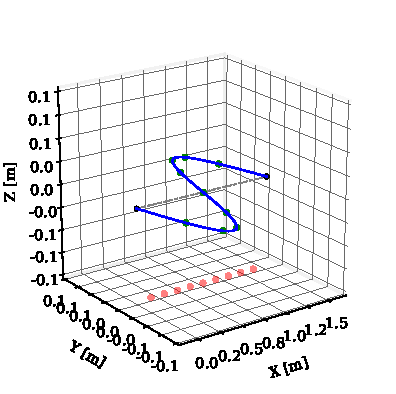
\includegraphics[width=0.35\linewidth]{/test_blue/blue_modes/fig_mod_8_time_22_11_45.pdf}%
				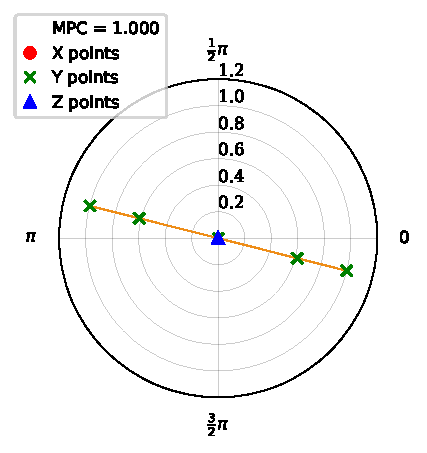
\includegraphics[width=0.3\linewidth]{/test_blue/polar/fig_polar_mod_8_time_22_11_32.pdf}%
		\end{tabular}}\\
		\subfloat[Mod 6, $f_6=205.290 \text{Hz}$]{\label{fig: test_blue_mod6}%
			\begin{tabular}[b]{c c c}
				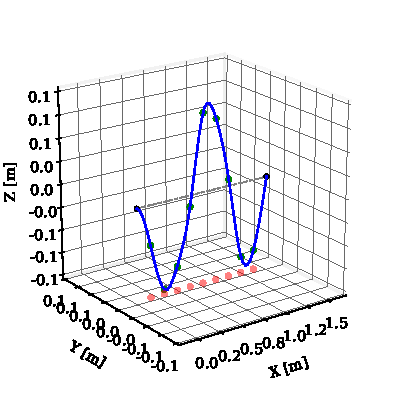
\includegraphics[width=0.35\linewidth]{/test_blue/blue_modes/fig_mod_10_time_22_12_47.pdf}%
				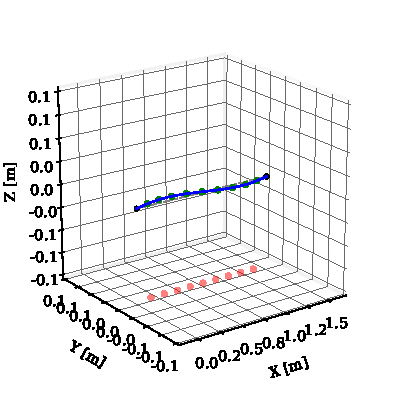
\includegraphics[width=0.35\linewidth]{/test_blue/blue_modes/fig_mod_10_time_22_12_15.pdf}%
				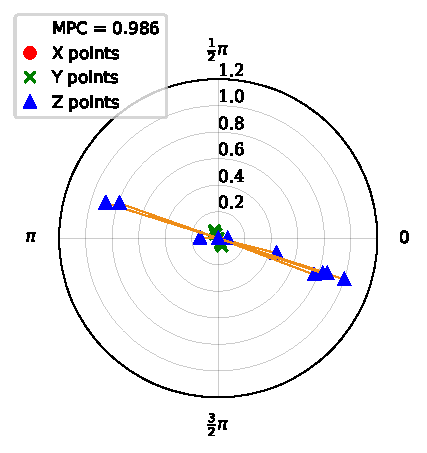
\includegraphics[width=0.3\linewidth]{/test_blue/polar/fig_polar_mod_10_time_22_14_19.pdf}%
		\end{tabular}}\\
		\subfloat[Mod 7, $f_7=310.834 \text{Hz}$]{\label{fig: test_blue_mod7}%
			\begin{tabular}[b]{c c c}
				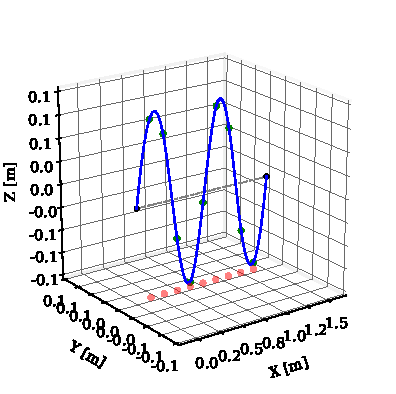
\includegraphics[width=0.35\linewidth]{/test_blue/blue_modes/fig_mod_16_time_22_21_41.pdf}%
				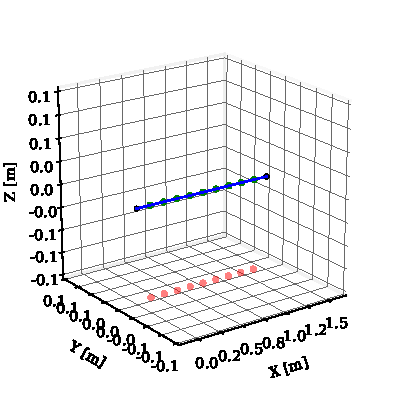
\includegraphics[width=0.35\linewidth]{/test_blue/blue_modes/fig_mod_16_time_22_22_09.pdf}%
				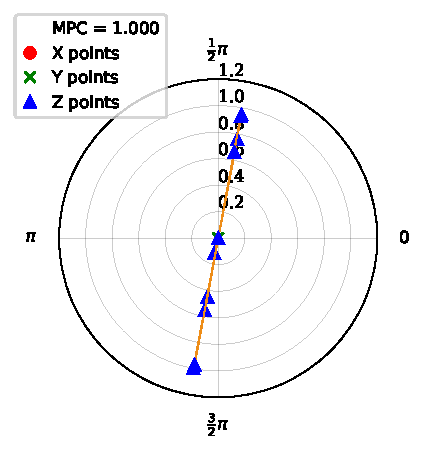
\includegraphics[width=0.3\linewidth]{/test_blue/polar/fig_polar_mod_16_time_22_21_32.pdf}%
		\end{tabular}}\\
		\subfloat[Mod 8, $f_8=384.619 \text{Hz}$]{\label{fig: test_blue_mod8}%
			\begin{tabular}[b]{c c c}
				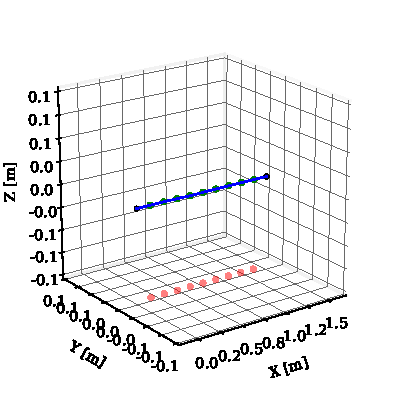
\includegraphics[width=0.35\linewidth]{/test_blue/blue_modes/fig_mod_24_time_22_22_41.pdf}%
				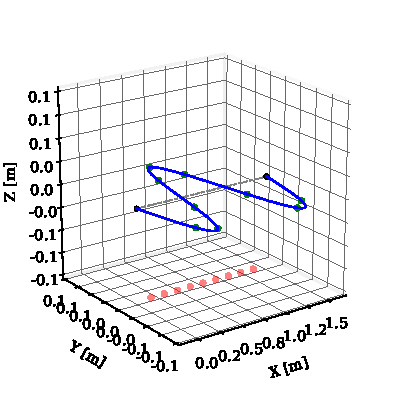
\includegraphics[width=0.35\linewidth]{/test_blue/blue_modes/fig_mod_24_time_22_22_48.pdf}%
				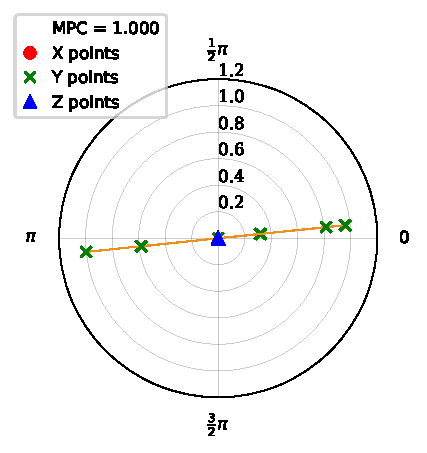
\includegraphics[width=0.3\linewidth]{/test_blue/polar/fig_polar_mod_24_time_22_22_25.pdf}%
		\end{tabular}}\\
	\end{tabular}
	\caption{Zidentyfikowane charakterystyki modalne belki testowej kont.}
\end{figure}






\subsection{Testy eksperymentalne metody NEXT-ERA} \label{sect: next_era_lab_test}
W warunkach laboratoryjnych wykonano pomiary na belce rzeczywistej (Rys. \ref{fig: blue_beam_lab_photo}). Belka została usytuowana na stabilnym podłożu. Aby ograniczyć możliwość przesuwu elementów podparcia w trakcie oddziaływania, punkty podparcia zostały dociążone ciężkimi stalowymi elementami. System pomiarowy składał się z wzmacniacza pomiarowego PMX firmy HBM (Hottinger Baldwin Messtechnik GmbH, Darmstadt, Germany), kabli i niskoszumnych, piezorezystywnych czujników akcelerometrycznych firmy TE CONNECTIVITY. Do obsługi wzmacniacza i akwizycji danych użyto program HBM Catman Easy. Czujniki przymocowano magnetycznie do belki. Zastosowano dwa czujniki 3-osiowe (traktowane jako 2-osiowe) i jeden 1-osiowy. Zakres pomiarowy akcelerometrów wynosi $\pm 2 \text{g}$, a gwarantowane szumy są określone jako mniejsze niż $25\mu \text{g RMS}$. Stanowisko pomiarowe zostało zaprezentowane na rysunku \ref{fig: blue_beam_lab_photo_a}, a szczegóły konstrukcyjne belki i jej podparcia na rysunku \ref{fig: blue_beam_lab_photo_b}
\begin{figure}[h]
	\centering
	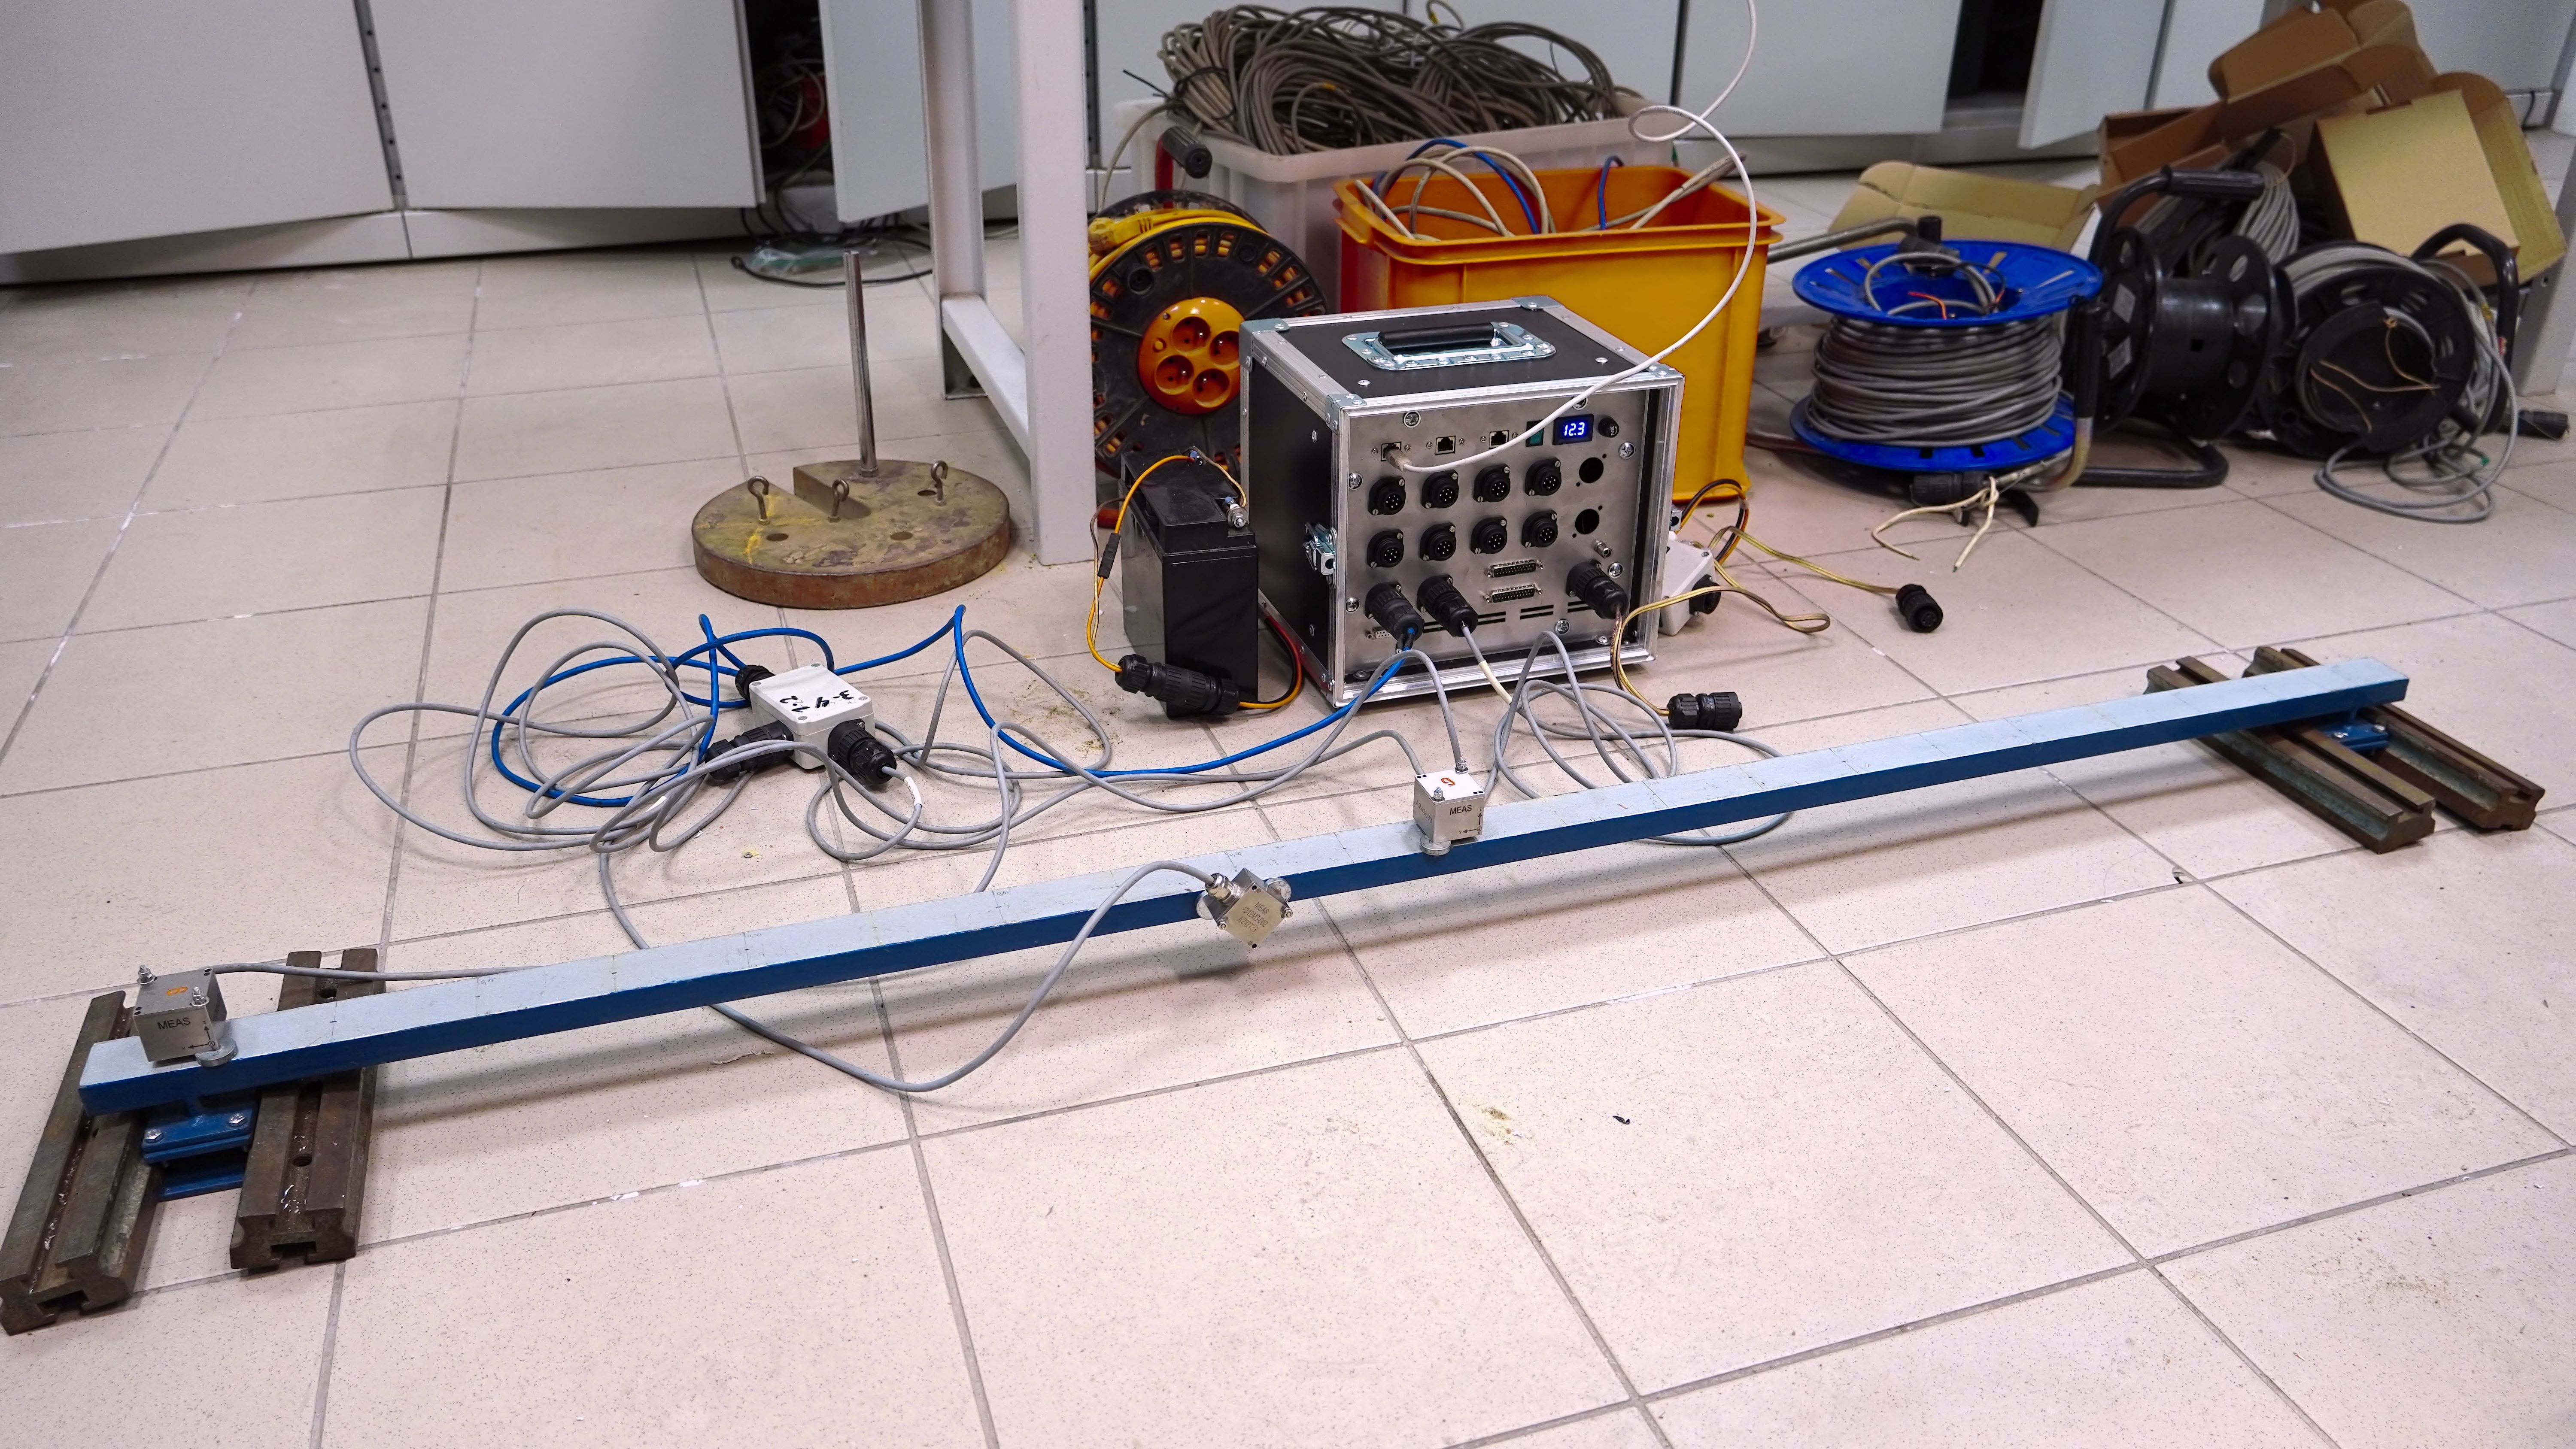
\includegraphics[width=0.3\textwidth]{/test_blue/lab_photo/DSC07487.jpg}
	\includegraphics[width=0.3\textwidth]{/test_blue/lab_photo/DSC07477_1.jpg}
	\includegraphics[width=0.3\textwidth]{/test_blue/lab_photo/DSC07502.jpg}
	\captionsetup{justification=centering}
	\caption{Szczegóły konstrukcyjne belki testowej}
	\label{fig: blue_beam_lab_photo_b}
\end{figure}
\begin{figure}[h]
\centering	
	\includegraphics[width=0.3\textwidth]{/test_blue/lab_photo/DSC07486.jpg}
	\includegraphics[width=0.3\textwidth]{/test_blue/lab_photo/DSC07500.jpg}
	\includegraphics[width=0.3\textwidth]{/test_blue/lab_photo/DSC07475.jpg}
	\captionsetup{justification=centering}
	\caption{Elementy aparatury pomiarowej}
	\label{fig: blue_beam_lab_photo_a}
\end{figure}



\subsubsection{Częstotliwość próbkowania}
Częstotliwość próbkowania $f_s$ określa jak często rejestrowana będzie wartość mierzona. Zwykle zakłada się równy odstęp pomiędzy próbkami $\Delta t$. W kontekście pomiarów dynamicznych konstrukcji ważne jest aby zarejestrować drgania o wszystkich interesujących częstotliwościach. Teoretycznie gwarantuje to przyjęcie dwukrotnie większej częstotliwości próbkowania $f_s$ niż najwyższa interesująca częstotliwość odpowiedzi układu $f_{max}$. Graniczna częstotliwość nazywa się częstotliwością Nyquista i wynosi $f_N = 0.5f_s$. Jednakże systemy akwizycji danych najczęściej posiadają filtry antyaliasingowe, które mają swoje odbicie w pobliżu częstotliwości Nyquista. \cite{Brincker2015} podają, że z tego względu częstotliwość Nyquista musi o 20\% większa niż wymagana teoretycznie. Podsumowując minimalna zaleca częstotliwość próbkowania powinna być równa:
\begin{equation} \label{eq: oma_min_sampling}
	f_s > 2.4 f_{max}
\end{equation}
Przyjmując założoną minimalną granicę interesujących modów jako 250Hz wyliczono częstotliwość próbkowania jako $f_{s,min}=2.4\cdot250\text{Hz}=600\text{Hz}.$ W badaniach przyjęto znacznie wyższą częstotliwość równą $f_s$=2400Hz chcąc, podobnie jak w przypadku modelu teoretycznego, móc zidentyfikować również kilka wyższych modów.
\subsubsection{Długość pomiarów}
Czas serii pomiarowej przyjęto zgodnie z zaleceniami opisanymi w \cite{Brincker2015}. Według autorów minimalny czas gwarantujący poprawne określenie tłumienia, bez ryzyka negatywnego wpływu obciążeń metody Welch'a, musi być dłuższy niż 20 okien czasowych użytych przy wyznaczeniu funkcji korelacji. Z tego względu zalecana minimalna długość pomiaru dana jest nierównością \ref{eq: minimum_oma_time_series}.
\begin{equation} \label{eq: oma_min_time_series}
	T_{tot} > \frac{20}{2\xi f_{min}}=\frac{10}{\xi f_{min}}
\end{equation}
gdzie $f_{min}$ oznacza najniższą częstotliwość drgań własnych układu. Dla podanego układu minimalna częstotliwość drgań własnych wyznaczona teoretycznie wynosi $f_{min}=19.7 \text{Hz}$, a przewidywana minimalna liczba tłumienia wynosi $\xi \approx 0.005$. Minimalna długość serii pomiarowej wynosi więc $T_{min} = \frac{10}{0.005\cdot 19.7} = 101.5 \text{s}$. 

\subsubsection{Stosunek sygnału do szumu pomiarowego}
Wyznaczono również stosunek poziomu sygnału do szumu posługując się wzorem:
\begin{equation} \label{eq: oma_dynamic_range}
	SN = 20 \log{\frac{\sigma_s}{\sigma_n}}
\end{equation}
gdzie $\sigma_s$ oznacza wartość RMS sygnału zmierzonego, a $\sigma_n$ jest wartością RMS szumu tła. Według zaleceń ANSI S2.47 wartość ta nie powinna być mniejsza niż 10 dB. \cite{Brincker2015} zalecają by w przypadku OMA stosunek sygnału do szumu nie był mniejszy niż 30-40 dB.

\subsubsection{Przebieg badań}
Przeprowadzono analizę sygnałów NExT-ERA podobnie jak miało to miejsce dla modelu numerycznego. Zastosowano dwa czujniki referencyjne. Jeden, mierzący pionowe i poprzeczne przyspieszenia w ciągu całych badań znajdował się w odległości 0.4L od podpory. Drugi, mierzący jedynie przyspieszenia poziome znajdował się w odległości 0.3L od podpory. Zwiększenie liczby czujników referencyjnych pozwala uniknąć sytuacji, gdzie jedyny czujnik referencyjny będzie znajdował się w węźle jakiegoś modu, co nie pozwoli go później zidentyfikować \parencite{Caicedo2011}. W takiej sytuacji drugi czujnik może w innym wariancie identyfikacji posłużyć jako referencyjny, a wyniki z obu wariantów należy scalić. Trzeci, ruchomy czujnik był przestawiany 10 razy tak, że ostatecznie zmierzono przyspieszenia na obu kierunkach w 11 punktach odpowiadających węzłom modelu numerycznego oraz punktom podporowym. . 


Pomiary odbywały się w pomieszczeniu, w godzinach wieczornych. Z tego powodu amplitudy przyspieszeń wywołane oddziaływaniem otoczenia były znikome. Dla zastosowanego układu pomiarowego zmierzony w laboratorium szum charakteryzuje się wartością RMS $\sigma_n=0.00138\,  \text{m}/\text{s}^2$. Sygnał nie zmieniał swojej mocy niezależnie od tego czy czujnik był umieszczony na obiekcie czy na stabilnym podłożu. Z tego względu w badaniach zastosowano sztuczne wymuszenie. \cite{Brincker2015} w przypadku badań laboratoryjnych zalecają szuranie lub gładzenie obiektu. W badaniach szurano po strukturze zgniecionym papierem pakowym. Wiotka struktura elementu wymuszającego nie powinna wpłynąć na dodatkowe tłumienie drgań. RMS jednominutowego sygnału pomierzonego ze sztucznym wymuszeniem wyniósł $\sigma_n=0.0539\,  \text{m}/\text{s}^2$. Dla takich rezultatów obliczony wg formuły (\ref{eq: oma_dynamic_range}) stosunek sygnału do szumu jest równy $SN = 20\log{\frac{0.0539}{0.0014}}=31.84\,\text{dB}$. Wyznaczona wartość jest większa niż zalecana.

\subsubsection{Rezultaty badań}
Diagramy stabilizacyjny metody NExT-ERA pokazano na rysunku \ref{fig: stab_diags_lab_blue_beam}. Zidentyfikowano 4 stabilne mody. Zidentyfikowane częstotliwości i postaci drgań zamieszczono na rysunku \ref{fig: blue_beam_research_mods}. Rezultaty porównano również z obliczeniami numerycznymi w tabeli \ref{tab: blue_beam_comparison}. 
\begin{figure}[h]
	\centering
	\subfloat[Diagram niefiltrowany]{\includegraphics[width=\linewidth]{/test_blue/stab_diag_lab/fig_stab_diagram_nonfiltr_time_17_49_58.pdf}}\\
	\subfloat[Diagram filtrowany]{\includegraphics[width=\linewidth]{/test_blue/stab_diag_lab/fig_stab_diagram_filtr_time_17_49_52.pdf}}%
	\captionsetup{justification=centering}
	\caption{Diagram stabilizacyjny metody NExT-ERA rzeczywistej belki testowej: (a) diagram niefiltrowany, (b) diagram filtrowany}
	\label{fig: stab_diags_lab_blue_beam}
\end{figure}

\begin{figure}[p]
	\centering
	\begin{tabular}[c]{c}
		\subfloat[Mod 1, $f_1=20.467 \text{Hz}$]{\label{fig: blue_beam_research_mod01}%
			\begin{tabular}[b]{c c c}
				\includegraphics[width=0.35\linewidth,trim=0 0 0 25,clip]{/test_blue/blue_modes_lab/fig_mod_0_time_18_20_13.pdf}%
				\includegraphics[width=0.35\linewidth,trim=0 0 0 25,clip]{/test_blue/blue_modes_lab/fig_mod_0_time_18_20_19.pdf}%
				\includegraphics[width=0.3\linewidth]{/test_blue/polar_lab/fig_polar_mod_0_time_18_20_26.pdf}%
		\end{tabular}}\\
		\subfloat[Mod 2, $f_2=22.236 \text{Hz}$]{\label{fig: blue_beam_research_mod02}%
			\begin{tabular}[b]{c c c}
				\includegraphics[width=0.35\linewidth,trim=0 0 0 25,clip]{/test_blue/blue_modes_lab/fig_mod_2_time_18_21_14.pdf}%
				\includegraphics[width=0.35\linewidth,trim=0 0 0 25,clip]{/test_blue/blue_modes_lab/fig_mod_2_time_18_21_24.pdf}%
				\includegraphics[width=0.3\linewidth]{/test_blue/polar_lab/fig_polar_mod_2_time_18_21_30.pdf}%
		\end{tabular}}\\
		\subfloat[Mod 3, $f_3=76.736 \text{Hz}$]{\label{fig: blue_beam_research_mod03}%
			\begin{tabular}[b]{c c c}
				\includegraphics[width=0.35\linewidth,trim=0 0 0 25,clip]{/test_blue/blue_modes_lab/fig_mod_8_time_18_20_48.pdf}%
				\includegraphics[width=0.35\linewidth,trim=0 0 0 25,clip]{/test_blue/blue_modes_lab/fig_mod_8_time_18_20_55.pdf}%
				\includegraphics[width=0.3\linewidth]{/test_blue/polar_lab/fig_polar_mod_8_time_18_20_59.pdf}%
		\end{tabular}}\\
		\subfloat[Mod 4, $f_4=163.584 \text{Hz}$]{\label{fig: blue_beam_research_mod04}%
			\begin{tabular}[b]{c c c}
				\includegraphics[width=0.35\linewidth,trim=0 0 0 25,clip]{/test_blue/blue_modes_lab/fig_mod_16_time_18_21_53.pdf}%
				\includegraphics[width=0.35\linewidth,trim=0 0 0 25,clip]{/test_blue/blue_modes_lab/fig_mod_16_time_18_21_58.pdf}%
				\includegraphics[width=0.3\linewidth]{/test_blue/polar_lab/fig_polar_mod_16_time_18_22_02.pdf}%
		\end{tabular}}\\
		
	\end{tabular}
	\caption{Zidentyfikowane charakterystyki modalne belki testowej}
	\label{fig: blue_beam_research_mods}
\end{figure}

Analizując rezultaty można zauważyć, że zidentyfikowano poprawnie 3 giętne pionowe postaci drgań. Pomimo bardzo dobrej zgodności częstotliwości i formy drgań ich tłumienie jest jednak znacząco większe niż zakładane LDT$=3\%$ w modelu numerycznym. Z uwagi na dużą wartość tłumienia dokonano prostej weryfikacji. Na rysunku \ref{fig: blue_beam_natural_vib} pokazano przyspieszenia pionowe środkowego punktu belki, drgającego swobodnie po wymuszeniu siłą impulsową. 
Sygnał odfiltrowano do 25Hz uzyskując drgania w pierwszej postaci. Odczytano wartości kolejnych amplitud o numerach 1, 10 i 20. Dla obu przedziałów 1-10 i 10-20 wyznaczono logarytmiczny dekrement tłumienia: $\textrm{LDT}_{1-10} = \frac{1}{10-1} \ln{\frac{3.156}{1.378}}=0.092 \quad
\textrm{LDT}_{10-20}=\frac{1}{20-10}\ln{\frac{1.378}{0.544}}=0.093$. Wyznaczone tłumienia są zbliżone do wartości wynikającej z analizy NExT-ERA.


\begin{figure}[h]
	\centering
	\includegraphics[trim=0 0 0 17,clip]{/test_blue/fig_00_12_14_0.978.pdf}
	\captionsetup{justification=centering}
	\caption{Odpowiedź swobodna belki testowej}
	\label{fig: blue_beam_natural_vib}
\end{figure}


 Jedyna giętna postać poprzeczna nie odpowiada strukturalnie żadnej z wyznaczonych w analizach numerycznych. Mimo to sklasyfikowano ją jako mod 2 w tabeli \ref{tab: blue_beam_comparison}. Charakteryzuje się ona ruchem wszystkich punków pomiarowych, w jednym kierunku i o zbliżonej amplitudzie. Dotyczy to także punków nad miejscami podparcia. Mimo to mod został zidentyfikowany jako stabilny i charakteryzuje się bardzo wysokim tłumieniem (LDT$=0.44$). Istnieje kilka elementów, które mogły wpłynąć na brak spodziewanej identyfikacji poziomych modów giętnych belki. Głównym jest różniąca się struktura fragmentów podporowych. Podpora belki laboratoryjnej była złożona z połączenia śrubowego i nie była sztywno przymocowana do podłoża. W modelu numerycznym w tym miejscu ustalono sztywne więzy w układzie belki swobodnie podpartej. Postać i wysokie tłumienie moda nr 2 może świadczyć, że belka wahała się na boki w całości i nie udało się wymusić drgań poprzecznych o bardzo wysokich częstotliwościach.

\section{Podsumowanie testów metody NExT-ERA}
Zidentyfikowane częstotliwości drgań własnych oraz tłumienia zestawiono w tabeli \ref{tab: blue_beam_comparison}. 

Częstotliwości wynikające z analizy modalnej i zidentyfikowane z odpowiedzi modelu numerycznego charakteryzują się bardzo dobrą zgodnością. Dla niskich częstotliwości różnice nie są większe niż 1\%. Wraz ze wzrostem częstotliwości wzrastają również różnice do maksymalnie 8\%. Jest to prawdopodobnie spowodowane zbyt niską częstotliwością próbkowania (zbyt dużym krokiem czasowym) dla modów o wysokich częstotliwościach. W takim przypadku różnica nie wynika z błędów identyfikacji tylko z błędów w wyznaczeniu odpowiedzi dynamicznej konstrukcji. Obserwując postaci uzyskane z analizy modalnej można zauważyć, że Mod 7 i Mod 10 mają charakter skrętny. Posługując się modelem belkowym i odczytując przyspieszenia węzłów wyłącznie na kierunku $Y$ i $Z$ nie ma możliwości zaobserwować tych postaci. Przeprowadzona identyfikacja potwierdza ten fakt, nie wskazując tych modów jako stabilnych rozwiązań. Z tego względu w tabeli zbiorczej zostały one oznaczone myślnikiem jako brakujące. Zidentyfikowane tłumienia różnią się do maksymalnie do 23\% od zakładanych wartości wynikających z formuł teoretycznych. Uzyskanie dobrej zgodności zidentyfikowanego tłumienia jest z reguły bardziej problematyczne niż ma to miejsce w przypadku częstotliwości. W przedmiotowym przypadku większość tłumień zidentyfikowanych nie różni się o więcej niż 10\% od wartości teoretycznych.

W badaniach laboratoryjnych zidentyfikowano 4 stabilne mody. Model numeryczny pomimo dobrego odwzorowania wymiarów geometrycznych konstrukcji nie był kalibrowany względem obiektu rzeczywistego. Niemniej, pomimo braku kalibracji modelu numerycznego, częstotliwości modów pionowych są bardzo bliskie wartościom z analizy modalnej. Maksymalna różnica wynosi 4\%. Tłumienia modów pionowych są zdecydowanie większe niż zakładane teoretycznie. Ich porównanie jest podane orientacyjnie i nie ma daje podstaw do wyciągnięcia wniosków na temat identyfikacji. Dla sprawdzenia efektu identyfikacji tłumienia w warunkach rzeczywistych porównano Logarytmiczny Dekrement Tłumienia odpowiedzi swobodnej układu ze zidentyfikowanym tłumieniem pierwszego modu (Rys. \ref{fig: blue_beam_natural_vib}). Stosunek obu wartości wynosi $\text{LDT}_{\text{ident}}/\text{LDT} = 0.097/0.093=1.04$. Zawarty w tabeli mod 2 nie ma odpowiednika w analizach teoretycznych co uzasadniono w punkcie \ref{sect: next_era_lab_test} i jego wystąpienie uznano za efekt niedoskonałego eksperymentu. Warto zaznaczyć, że mod 1 i mod 2 są bliskie pod względem częstotliwości przy zastosowanym spektrum całkowitym, a ich identyfikacja i rozróżnienie nie sprawiło problemu.
Podsumowując, na podstawie przytoczonych testów uznano zaimplementowany algorytm jako skuteczny i przystąpiono do badań właściwych. Identyfikacja modalna rzeczywistego obiektu mostowego została opisana w punkcie \ref{sect: identyfikacja_modalna_wk2}.

%\resizebox{\textwidth}{!}{%
% Please add the following required packages to your document preamble:
% \usepackage{booktabs}
\begin{table}[]
	\caption{Porównanie zidentyfikowanych parametrów modalnych obiektu testowego}
	\label{tab: blue_beam_comparison}
	\resizebox{\textwidth}{!}{%
	\begin{tabular}{@{}c|c|c|cccc|cccc@{}}
		\toprule
		\multicolumn{1}{l|}{} & \textbf{\begin{tabular}[c]{@{}c@{}}Analiza\\ modalna\end{tabular}} & \textbf{\begin{tabular}[c]{@{}c@{}}Zakładane\\ tłumienie\end{tabular}} & \multicolumn{4}{c|}{\textbf{Model MES}}                                      & \multicolumn{4}{c}{\textbf{Badania}}                                        \\ \midrule
		\multicolumn{1}{l|}{} & \textbf{Częst.}                                                    & \textbf{LDT}                                                           & \textbf{Częst.}   & \textbf{Stosunek} & \textbf{LDT}     & \textbf{Stosunek} & \textbf{Częst.}   & \textbf{Stosunek} & \textbf{LDT}     & \textbf{Stosunek} \\ \midrule
		\multicolumn{1}{l|}{} & \textbf{{[}Hz{]}}                                                  & \textbf{{[}-{]}}                                                       & \textbf{{[}Hz{]}} & \textbf{{[}\%{]}} & \textbf{{[}-{]}} & \textbf{{[}\%{]}} & \textbf{{[}Hz{]}} & \textbf{{[}\%{]}} & \textbf{{[}-{]}} & \textbf{{[}\%{]}} \\ \midrule
		\textbf{Mod 1}        & 19.77                                                              & 0.0303                                                                 & 19.701            & 100\%             & 0.0291           & 96\%              & 20.467            & 104\%             & 0.097            & 333\%             \\ \midrule
		\textbf{Mod 2}        & 54.93                                                              & 0.0189                                                                 & 54.958            & 100\%             & 0.0232           & 123\%             & 22.236            & 40\%              & 0.440            & 2335\%            \\ \midrule
		\textbf{Mod 3}        & 78.20                                                              & 0.0199                                                                 & 77.331            & 99\%              & 0.0190           & 96\%              & 76.739            & 98\%              & 0.151            & 760\%             \\ \midrule
		\textbf{Mod 4}        & 161.35                                                             & 0.0302                                                                 & 157.995           & 98\%              & 0.0240           & 79\%              & 163.584           & 101\%             & 0.185            & 614\%             \\ \midrule
		\textbf{Mod 5}        & 200.38                                                             & 0.0361                                                                 & 197.881           & 99\%              & 0.0325           & 90\%              & -                 & -                 & -                & -                 \\ \midrule
		\textbf{Mod 6}        & 212.24                                                             & 0.0379                                                                 & 205.29            & 97\%              & 0.0410           & 108\%             & -                 & -                 & -                & -                 \\ \midrule
		\textbf{Mod 7}        & 217.12                                                             & 0.0386                                                                 & -                 & -                 & -                & -                 & -                 & -                 & -                & -                 \\ \midrule
		\textbf{Mod 8}        & 336.59                                                             & 0.0577                                                                 & 310.834           & 92\%              & 0.0473           & 82\%              & -                 & -                 & -                & -                 \\ \midrule
		\textbf{Mod 9}        & 410.22                                                             & 0.0697                                                                 & 384.619           & 94\%              & 0.0628           & 90\%              & -                 & -                 & -                & -                 \\ \midrule
		\textbf{Mod 10}       & 451.89                                                             & 0.0765                                                                 & -                 & -                 & -                & -                 & -                 & -                 & -                & -                 \\ \bottomrule
	\end{tabular}}
\end{table}